\documentclass{common/template}

\TemplateDefineDocumentVersion{TestNet V1 (\gitbranch /\gitrevision)}
% \TemplateDefineDocumentSecurity{Draft/Confidential}
\TemplateDefineDocumentSecurity{}
\TemplateDefineDocumentType{Specification}

% Watermark indicator. Delete this, if a version is ready to publish
% \watermark{Draft}
% \renewcommand{\todo}{}  % uncomment to hide TODO-s

% The title of the document
\title{Unicity Yellowpaper}

% Authors
\author{The Unicity Team}

% Date
\date{\today}

% Definitions
\newcommand{\embl}[1]{\textcolor{blue}{#1}}

\usepackage{pgf-umlsd}
\usetikzlibrary{positioning}

\newenvironment{leveldown}% Demote sectional commands
  {\let\chapter\section%
   \let\section\subsection%
   \let\subsection\subsubsection%
   \let\subsubsection\paragraph%
   \let\paragraph\subparagraph%
   %\let\subparagraph\relax%
  }{}
\newenvironment{levelup}% Promote sectional commands
  {\let\subparagraph\paragraph%
   \let\paragraph\subsubsection%
   \let\subsubsection\subsection%
   \let\subsection\section%
   \let\section\chapter%
   %\let\section\relax%
  }{}

%
% General notation
%

\newcommand{\uint}[1]{\mathbb{N}_{#1}}
\newcommand{\bool}{\mathbb{B}}

\newcommand{\bits}[1]{\{0,1\}^{#1}}
\newcommand{\bitstr}{\bits{\ast}}
\newcommand{\emptystr}{\lfloor\!\rfloor}

\newcommand{\bytes}[1]{\mathbb{OCT}^{#1}}
\newcommand{\bytestr}{\bytes{\ast}}

\newcommand{\chars}[1]{\mathbb{CHR}^{#1}}
\newcommand{\charstr}{\chars{\ast}}

\newcommand{\len}[1]{\left|#1\right|}

% convenience macro to add "or none" to a type to mark a field optional
\newcommand{\opt}{\cup\{\bot\}}

\newcommand{\hashtype}{\mathbb{H}}
\newcommand{\zerohash}{\bot}

\newcommand{\idtype}{\mathbb{I}}
\newcommand{\zeroid}{\bot}

%
% Platform
%

\newcommand{\prndsh}{\mathsf{PrndSh}}

\newcommand{\nodeid}{\mathsf{NodeID}}
\newcommand{\extrtype}{\mathsf{ExtrType}}
\newcommand{\extrunit}{\mathsf{ExtrUnit}}

\newcommand{\additem}{\mathsf{AddItem}}
\newcommand{\delitem}{\mathsf{DelItem}}

%
% Execution Layer
%

\newcommand{\sthash}{{h_\mathsf{st}}}
\newcommand{\txhash}{{h_\mathsf{tx}}}
\newcommand{\auxd}{\mathsf{aux}}
\newcommand{\predi}{\nu}
\newcommand{\unisrv}{\mathsf{US}}
\newcommand{\certver}{{\mathcal{V}_\mathsf{cert}}}
\newcommand{\pinc}{{\pi_\mathsf{inc}}}


\begin{document}
\maketitle

\pagebreak
% Creates the table of contents
\setcounter{tocdepth}{4}
% \setcounter{secnumdepth}{4}  % 4th level is not numbered by default
\makeatletter
\renewcommand\@pnumwidth{0.7cm} % accommodate 3-digit page numbers
\makeatother
\tableofcontents*{}

%\input{common/notation}

\chapter{General Description}

\section{System Architecture}

The Unicity protocol employs a hierarchical three-layer architecture designed for scalability and decentralization. Each layer serves a distinct function in the system:

\begin{figure}[!htbp]
    \centering
        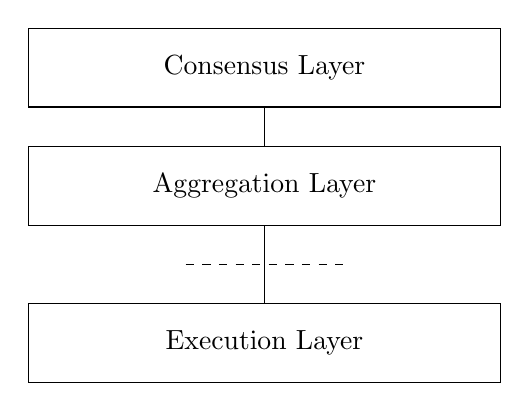
\begin{tikzpicture}
            \draw (0,0) rectangle (6,1) node[midway] {Consensus Layer};
            \draw (3,0) -- (3,-0.5);
            \draw (0,-1.5) rectangle (6,-0.5) node[midway] {Aggregation Layer};
            \draw[dashed] (2,-2) -- (4,-2);
            \draw (3,-1.5) -- (3,-2.5);
            \draw (0,-3.5) rectangle (6,-2.5) node[midway] {Execution Layer};
        \end{tikzpicture}
    \caption{Hierarchical architecture of the Unicity Network.}\label{fig:unicity-layers}
\end{figure}

\begin{description}
\item[Consensus Layer] PoW chain and BFT Core. Provides token minting, decentralized agreement and finality through Byzantine Fault Tolerant consensus. This layer verifies the integrity of the Aggregation Layer's state transitions and serves as the root of trust for the entire system. The BFT Core certifies SMT root hashes submitted by the aggregation layer.

\item[Aggregation Layer] Maintains a global append-only registry of spent token states using sharded Sparse Merkle Trees (SMT). Each partition within this layer processes state certification requests, provides inclusion proofs, and uses consistency proofs to enable trustless verification. The layer is organized into partitions for service design flexibility, with each partition potentially divided into shards for horizontal scalability.

\item[Execution Layer] Handles off-chain transaction processing and business logic. Token transactions occur peer-to-peer between users, with only cryptographic commitments to state transitions submitted to the Aggregation Layer for certification. This design moves computational overhead off-chain while maintaining trustless double-spending prevention.
\end{description}

The BFT Core certifies state transitions by cryptographically signing the root hashes of the Aggregation Layer's SMTs. This hierarchical design enables linear scalability: the BFT Core's throughput requirements grow only with the number of shards, not with the number of transactions processed by the system.


\chapter{Execution Layer}

The execution layer handles off-chain transaction processing and business logic. Tokens are self-contained digital assets transferred peer-to-peer between users. Only cryptographic commitments to state transitions are submitted to the Aggregation Layer for double-spending prevention. Transaction execution and verification are performed by the interested parties (recipients), not by consensus participants. This design moves computational overhead off-chain while maintaining trustless guarantees against double-spending.

\section{Execution Model}

In the Unicity execution model, digital assets called \emph{tokens}\index{token} are bearer instruments: whoever holds the token data and can satisfy the spending condition is the owner. Transactions occur directly between parties using any communication channel, with the Unicity Service consulted only to prevent double-spending.

The model relies on three key principles:
\begin{enumerate}
	\item \textbf{Off-chain execution}: Transaction creation, validation, and verification happen between sender and recipient without consensus participation.
	\item \textbf{On-chain uniqueness}: The Unicity Service maintains an append-only registry of spent token states, ensuring each state can be spent at most once.
	\item \textbf{Recipient verification}: The recipient (relying party) independently verifies the complete token history before accepting a transfer.
\end{enumerate}

\subsection{Token Lifecycle}\label{sec:token-lifecycle}

A token progresses through the following stages:
\begin{description}
\item[Minting]\index{mint transaction} Creates a new token with an initial state. Minting uses a publicly known minting key $\mathsf{pk}_\mathsf{mint}$ (with publicly known private key $\mathsf{sk}_\mathsf{mint}$) to provide a unified interface with the Unicity Service.
\item[Transfer]\index{transfer transaction} Changes ownership by spending the current state and creating a new state with a new owner predicate.
\item[Compression]\index{token compression} Compacts the token by replacing a set of transactions with a cryptographic proof of validity of these transactions.
\item[Split]\index{split transaction} (Fungible tokens only.) Burns the original token and mints new tokens, with a cryptographic value conservation proof ensuring no value is created or destroyed. See Sec.~\ref{sec:token-splitting}.
\item[Burn]\index{burn transaction} Permanently locks a token by transferring it to a burn predicate that cannot be unlocked. See Sec.~\ref{sec:burn-transaction}.
\end{description}

\subsection{Token State}\label{sec:token-state}

\index{token!state}
A \emph{token state} is a pair $(\predi, \sthash)$, where:
\begin{itemize}
	\item $\predi$ -- the spending predicate (defines who can spend the token); see Sec.~\ref{sec:predicates}
	\item $\sthash \in \hashtype$ -- the state hash, linking the token's transaction history
\end{itemize}

The \emph{state identifier}\index{state identifier}\index{$\mathsf{sid}$ (state identifier)} is the key used in the Unicity Service registry:
\[
\mathsf{sid} = H(\predi, \sthash)
\]

When a transaction with random value $x \gets \{0,1\}^\ell$ is executed, the next state hash is computed as:
\[
\sthash' = H(\sthash, x)
\]

The randomness of $x$ ensures that the next state identifier $H(\predi', \sthash')$ is unpredictable, preventing the Unicity Service from linking consecutive states of the same token.

\subsection{Token Structure}\label{sec:token-structure}

A \emph{token}\index{token!structure} is a self-contained data structure carrying its complete provenance. Any party can independently verify the entire history without consulting external state. Formally, a token is a sequence:
\[
\mathcal{L} = (T_0^\mathsf{cert}, T_1^\mathsf{cert}, \ldots, T_n^\mathsf{cert})
\]
where $T_0^\mathsf{cert}$ is a certified mint transaction and $T_i^\mathsf{cert}$ for $i > 0$ are certified transfer transactions.

\subsubsection{Mint Transaction}\label{sec:mint-tx}

\index{mint transaction!structure}
A \emph{certified mint transaction} is a tuple $(T_0, u_0, \pi_0)$, where $T_0 = (\sthash, D_\mathsf{mint})$:
\begin{itemize}
	\item $\sthash = H(\mathsf{id}, \mathsf{MINT\_SUFFIX})$ -- source state hash, domain-separated from the token identifier
	\item $D_\mathsf{mint}$ -- mint transaction data, containing:
	\begin{itemize}
		\item $\mathsf{id} \in \idtype$ -- token identifier (globally unique)
		\item $\mathsf{ty}$ -- token type identifier, classifying the token category
		\item $\predi'$ -- spending predicate of the first owner
		\item $\auxd'$ -- auxiliary data (application-specific; e.g. mint justification, asset values for fungible tokens)
	\end{itemize}
	\item $u_0$ -- unlocking argument (signature with $\mathsf{sk}_\mathsf{mint}$)
	\item $\pi_0$ -- inclusion proof from the Unicity Service
\end{itemize}

$\mathsf{MINT\_SUFFIX}$\index{MINT\_SUFFIX} is a fixed domain separator constant (see Appendix~\ref{app:el-constants}). The minting key pair $(\mathsf{sk}_\mathsf{mint}, \mathsf{pk}_\mathsf{mint})$ is publicly known; it serves only to provide a uniform request interface with the Unicity Service.

\paragraph{Certifying a mint transaction} $T_0 = (\sthash, D_\mathsf{mint})$:
\begin{enumerate}
	\item $\txhash \gets H(D_\mathsf{mint})$
	\item $h_T \gets H(\sthash, \txhash)$
	\item $\sigma \gets \mathsf{Sign}(\mathsf{sk}_\mathsf{mint}, h_T)$
	\item $Q \gets (\mathsf{pk}_\mathsf{mint}, \sthash, \txhash, \sigma)$
	\item $\pi_0 \gets \unisrv(Q)$
\end{enumerate}

\paragraph{Verifying a certified mint transaction} $(T_0, u_0, \pi_0)$:
\begin{enumerate}
	\item $T_0.\sthash = H(T_0.D_\mathsf{mint}.\mathsf{id}, \mathsf{MINT\_SUFFIX})$
	\item $\mathsf{Verify}(\mathsf{pk}_\mathsf{mint}, H(\sthash, \txhash), u_0) = 1$, where $\txhash = H(D_\mathsf{mint})$
	\item $\mathcal{V}(H(\mathsf{pk}_\mathsf{mint}, \sthash), \txhash, \pi_0) = 1$
	\item Token type-specific checks on $\auxd'$ (e.g. mint justification validity)
\end{enumerate}


\subsubsection{Transfer Transaction}\label{sec:transfer-tx}

\index{transfer transaction!structure}
A \emph{certified transfer transaction} is a tuple $(T, u, \txhash, \pi)$, where $T = (\sthash, D)$:
\begin{itemize}
	\item $D = (\predi', x, \auxd')$ -- transaction data:
	\begin{itemize}
		\item $\predi'$ -- spending predicate of the next owner
		\item $x \gets \{0,1\}^\ell$ -- random value for state hash derivation
		\item $\auxd'$ -- auxiliary data for the next state
	\end{itemize}
	\item $\txhash = H(D)$ -- transaction data hash
	\item $u$ -- unlocking argument satisfying the current predicate $\predi$
	\item $\pi$ -- inclusion proof from the Unicity Service
\end{itemize}

\paragraph{Certifying a transfer transaction} $T = (\sthash, D)$ in the current state $(\predi, h)$:
\begin{enumerate}
	\item $\txhash \gets H(D)$
	\item $h_T \gets H(\sthash, \txhash)$
	\item Create $u$ such that $\predi(\tau_\mathsf{exp}, h_T, u) = 1$ for an expected system time $\tau_\mathsf{exp}$
	\item $Q \gets (\predi, \sthash, \txhash, u)$
	\item $\pi \gets \unisrv(Q)$
\end{enumerate}

\paragraph{Verifying a certified transfer transaction} $(T, u, \txhash, \pi)$ in state $(\predi, h)$:
\begin{enumerate}
	\item $T.\sthash = h$ \quad (state hash matches expected)
	\item $\predi(\mathsf{time}(\pi), H(\sthash, \txhash), u) = 1$ \quad (predicate satisfied)
	\item $\mathcal{V}(H(\predi, T.\sthash), \txhash, \pi) = 1$ \quad (inclusion proof valid)
	\item Additional token type-specific checks
\end{enumerate}

\subsection{Token Verification}\label{sec:token-verification}

\index{token!verification}\index{functions!VerifyToken}
$\mathsf{VerifyToken}$ -- token verification function of type $\mathbb{L} \times \mathbb{UB} \to \bool$

\textbf{Input}:
\begin{enumerate}
	\item $\mathcal{L} = (T_0^\mathsf{cert}, T_1^\mathsf{cert}, \ldots, T_n^\mathsf{cert})$ -- token
	\item $\mathcal{T}$ -- trust base
\end{enumerate}

\textbf{Output}: \TRUE or \FALSE

\textbf{Computation}:
\begin{algorithmic}[0]
	\State \Parse $T_0^\mathsf{cert}$ \textbf{as} $(T_0, u_0, \pi_0)$
	\If {$\neg \Call{VerifyMintTransaction}{T_0, u_0, \pi_0, \mathcal{T}}$} \Return \FALSE \EndIf
	\State $\predi^0 \gets T_0.D_\mathsf{mint}.\predi'$
	\State $h^0 \gets H(T_0.D_\mathsf{mint}.\mathsf{id}, \mathsf{MINT\_SUFFIX})$
	\For {$i \gets 1 \ldots n$}
		\State \Parse $T_i^\mathsf{cert}$ \textbf{as} $(T_i, u_i, \txhash_i, \pi_i)$
		\If {$\neg \Call{VerifyTransferTransaction}{T_i, u_i, \txhash_i, \pi_i, \predi^{i-1}, h^{i-1}, \mathcal{T}}$} \Return \FALSE \EndIf
		\State $\predi^{i} \gets T_i.D.\predi'$
		\State $h^{i} \gets H(h^{i-1}, T_i.D.x)$
	\EndFor
	\State \Return \TRUE
\end{algorithmic}


\section{Programmable Spending Conditions}\label{sec:predicates}

Instead of restricting ownership to a single public key, the Unicity execution layer generalizes ownership to \emph{predicates}\index{predicate} -- programmable boolean functions that define the conditions under which a token state can be spent. This enables smart-contract-like functionality executed off-chain by relying parties rather than by consensus participants.

\subsection{Predicate Framework}\label{sec:predicate-framework}

\index{predicate!framework}
A \emph{predicate} $\predi_\mathsf{name}(\mathsf{par}; \cdot)$ is a boolean function with:
\begin{itemize}
	\item \textbf{Name} $\mathsf{name}$ -- identifies the predicate type
	\item \textbf{Parameters} $\mathsf{par}$ -- type-dependent configuration (e.g. a public key)
	\item \textbf{Arguments} $(\tau, m, u)$:
	\begin{itemize}
		\item $\tau \in \mathbb{T}$ -- system time, extracted from the Unicity Seal timestamp $C^\mathsf{r}.t_r$
		\item $m \in \hashtype$ -- message hash $H(\sthash, \txhash)$
		\item $u$ -- unlocking argument, structure depends on predicate type
	\end{itemize}
\end{itemize}

The predicate evaluates to $\predi_\mathsf{name}(\mathsf{par}; \tau, m, u) \in \{0, 1\}$. The Unicity Service evaluates the predicate at the current system time $\tau$ when processing a certification request. Verifiers of certified transactions evaluate the predicate at the system time $\mathsf{time}(\pi)$ extracted from the inclusion proof.

\subsection{Standard Predicates}\label{sec:standard-predicates}

\subsubsection{Signature Predicate}

\index{predicate!signature ($\predi_\mathsf{sig}$)}
The \emph{signature predicate} $\predi_\mathsf{sig}(\mathsf{pk};\cdot)$ with a single public key $\mathsf{pk}$ as parameter is equivalent to digital signature verification. This is the basic ``pay to public key'' ownership model.

\begin{itemize}
	\item \textbf{Parameters}: $\mathsf{pk}$ (public key)
	\item \textbf{Unlocking argument}: $u = \sigma$ (digital signature)
	\item \textbf{Definition}: $\predi_\mathsf{sig}(\mathsf{pk}; \tau, m, \sigma) = 1$ iff $\mathsf{Verify}(\mathsf{pk}, m, \sigma) = 1$
\end{itemize}

\subsubsection{P2PKH Predicate}

\index{predicate!P2PKH ($\predi_\mathsf{p2pkh}$)}
The \emph{Pay-to-Public-Key-Hash} predicate $\predi_\mathsf{p2pkh}(h_\mathsf{pk};\cdot)$ stores only the hash of the public key, requiring the spender to reveal the full public key alongside the signature.

\begin{itemize}
	\item \textbf{Parameters}: $h_\mathsf{pk} \in \hashtype$ (public key hash)
	\item \textbf{Unlocking argument}: $u = (\mathsf{pk}, \sigma)$
	\item \textbf{Definition}: $\predi_\mathsf{p2pkh}(h_\mathsf{pk}; \tau, m, (\mathsf{pk}, \sigma)) = 1$ iff $H(\mathsf{pk}) = h_\mathsf{pk} \;\land\; \mathsf{Verify}(\mathsf{pk}, m, \sigma) = 1$
\end{itemize}

\subsubsection{P2SH Predicate}\label{sec:p2sh}

\index{predicate!P2SH ($\predi_\mathsf{p2sh}$)}
The \emph{Pay-to-Script-Hash} predicate $\predi_\mathsf{p2sh}(h_\predi;\cdot)$ generalizes P2PKH by storing the hash of an arbitrary predicate rather than just a public key hash. The recipient is identified by $h_\predi = H(\mathsf{CBOR}(\predi'))$, which provides a uniform-size recipient field regardless of predicate complexity and preserves privacy by hiding the predicate type until the token is spent.

\begin{itemize}
	\item \textbf{Parameters}: $h_\predi \in \hashtype$ (predicate hash)
	\item \textbf{Unlocking argument}: $u = (\predi', u')$ where $\predi'$ is the full predicate and $u'$ is its unlocking argument
	\item \textbf{Definition}: $\predi_\mathsf{p2sh}(h_\predi; \tau, m, (\predi', u')) = 1$ iff $H(\mathsf{CBOR}(\predi')) = h_\predi \;\land\; \predi'(\tau, m, u') = 1$
\end{itemize}

When spending, the full predicate $\predi'$ is revealed in the lock script field of the transfer transaction, and verifiers check that $H(\mathsf{CBOR}(\predi'))$ matches the recipient hash from the previous transaction.

\subsubsection{Multi-Signature Predicate}

\index{predicate!multi-signature ($\predi_\mathsf{msig}$)}
The \emph{multi-signature predicate} $\predi_\mathsf{msig}(\mathsf{pk}_1, \ldots, \mathsf{pk}_n;\cdot)$ requires $n$ valid signatures from $n$ specified public keys (all-of-$n$).

\begin{itemize}
	\item \textbf{Parameters}: $(\mathsf{pk}_1, \ldots, \mathsf{pk}_n)$
	\item \textbf{Unlocking argument}: $u = (\sigma_1, \ldots, \sigma_n)$
	\item \textbf{Definition}: $\predi_\mathsf{msig}(\mathsf{pk}_1, \ldots, \mathsf{pk}_n; \tau, m, u) = 1$ iff $\mathsf{Verify}(\mathsf{pk}_i, m, \sigma_i) = 1$ for every $i \in \{1, \ldots, n\}$
\end{itemize}


\subsubsection{Threshold-Signature Predicate}

\index{predicate!threshold-signature ($\predi_\mathsf{tsig}$)}
The \emph{threshold-signature predicate} $\predi_\mathsf{tsig}(k, \mathsf{pk}_1, \ldots, \mathsf{pk}_n;\cdot)$ requires $k$-of-$n$ valid signatures from distinct public keys.

\begin{itemize}
	\item \textbf{Parameters}: $(k, \mathsf{pk}_1, \ldots, \mathsf{pk}_n)$ where $k \in \{1, \ldots, n\}$
	\item \textbf{Unlocking argument}: $u = ((\sigma_1, j_1), \ldots, (\sigma_k, j_k))$ where $j_i$ is the index of the public key used for $\sigma_i$
	\item \textbf{Definition}: $\predi_\mathsf{tsig}(k, \mathsf{pk}_1, \ldots, \mathsf{pk}_n; \tau, m, u) = 1$ iff:
	\begin{enumerate}
		\item $\mathsf{Verify}(\mathsf{pk}_{j_i}, m, \sigma_i) = 1$ for every $i \in \{1, \ldots, k\}$
		\item All indices $j_i$ are distinct: $j_i = j_{i'}$ implies $i = i'$
	\end{enumerate}
\end{itemize}

The distinctness requirement prevents satisfying the predicate by presenting $k$ copies of the same signature.


\subsubsection{Burn Predicate}\label{sec:burn-predicate}

\index{predicate!burn ($\predi_\mathsf{burn}$)}
The \emph{burn predicate} $\predi_\mathsf{burn}(h_\mathsf{reason})$ cannot be unlocked. A token transferred to a burn predicate is permanently spent.

\begin{itemize}
	\item \textbf{Parameters}: $h_\mathsf{reason} \in \hashtype$ (reason hash, linking the burn to its purpose)
	\item \textbf{Unlocking argument}: none
	\item \textbf{Definition}: $\predi_\mathsf{burn}(h_\mathsf{reason}; \tau, m, u) = 0$ for all arguments
\end{itemize}

The burn predicate is used in token splitting (Sec.~\ref{sec:token-splitting}), where the reason hash references the aggregation root of the split proof.

\bigskip

Predicates can also encode time-dependent conditions, enabling protocols such as atomic swaps via hashed timelock predicates. Such application-level predicates are outside the scope of this specification.


\section{Interaction with Unicity Service}\label{sec:el-us-interaction}

\index{Unicity Service!execution layer interaction}
This section describes how the execution layer interacts with the Unicity Service (Sec.~\ref{sec:request-validation}) for state transition certification.

\subsection{Certification Request}

A certification request from the execution layer is a tuple $Q = (\predi, \sthash, \txhash, u)$, where:
\begin{itemize}
	\item $\predi$ -- spending predicate of the current owner
	\item $\sthash$ -- current state hash
	\item $\txhash$ -- transaction data hash
	\item $u$ -- unlocking argument satisfying $\predi$
\end{itemize}

\subsection{Processing}

The Unicity Service processes the request as follows:
\begin{enumerate}
	\item Compute state identifier: $\mathsf{sid} \gets H(\predi, \sthash)$
	\item Compute message hash: $m \gets H(\sthash, \txhash)$
	\item Evaluate predicate: verify $\predi(\tau, m, u) = 1$
	\item Check uniqueness: verify $R[\mathsf{sid}] = \bot$
	\item If both checks pass: $R[\mathsf{sid}] \gets \txhash$\footnote{The current SDK implementation stores $H(\mathsf{CBOR}(\predi, \sthash, \txhash, u))$ as the leaf value instead of $\txhash$, because of backward compatibility with the legacy SDK.}
\end{enumerate}

If the request is accepted, the Unicity Service returns an inclusion proof $\pinc$. If the state has already been spent (uniqueness check fails) or the predicate evaluation fails, the request is rejected.

\subsection{System Time}\label{sec:system-time}

\index{system time}
The system time $\tau$ available during predicate evaluation is the round creation time from the Unicity Seal: $\tau = C^\mathsf{r}.t_r$ (Sec.~\ref{se:unicity-certificate}). The system time can be extracted from inclusion proofs by $\tau \gets \mathsf{time}(\pi)$.

The Unicity Service evaluates predicates at the current round time. Verifiers of certified transactions evaluate predicates using the time extracted from the inclusion proof $\pi$.


\section{Transaction Flow}\label{sec:transaction-flow}

Figure~\ref{fi:exec-transaction-flow} illustrates one complete token transfer, from the recipient preparing ownership information through certification to final verification.

\begin{figure}[!htb]
    \begin{center}
        \begin{sequencediagram}
            \newthread{S}{Sender}
            \newinst[3]{R}{Recipient}
            \newinst[2]{US}{Unicity Service}

            % Recipient prepares predicate and auxiliary data
            \begin{call}{R}{Prepare $\predi'$, $\auxd'$}{R}{}
            \end{call}

            % Recipient sends predicate to sender
            \begin{messcall}{R}{$\predi'$, $\auxd'$}{S}
            \end{messcall}

            % Sender creates transaction data
            \postlevel
            \postlevel
            \postlevel
            \begin{call}{S}{\shortstack[l]{
                    $x \gets \{0,1\}^\ell$     \\
                    $D = (\predi', x, \auxd')$ \\
                    $T = (\sthash, D)$         \\
                    $\txhash \gets H(D)$ \\
                    $h_T = H(\sthash, \txhash)$ \\
                    $u$ such that $\predi(\tau_\mathsf{exp}, h_T, u) = 1$
                }
                }{S}{}
            \end{call}

            % Sender requests certification from Unicity Service
            \begin{messcall}{S}{$Q = (\predi, \sthash, \txhash, u)$}{US}
                \postlevel
                \begin{call}{US}{\shortstack[l]{
                    $\predi(\tau, H(\sthash, \txhash), u) \stackrel{?}{=} 1$ \\
                    $R[H(\predi, \sthash)] \stackrel{?}{=} \bot$ \\
                    $R[H(\predi, \sthash)] \gets \txhash$
                    }}{US}{}
                \end{call}
            \end{messcall}
            \prelevel
            \begin{messcall}{US}{$\pinc$ (with $\tau$)}{S}
            \end{messcall}

            % Sender sends certified transaction to recipient
            \begin{messcall}{S}{$\mathcal{L} \cup (T, u, \txhash, \pinc)$}{R}
                \postlevel
                \postlevel
                \postlevel
                \postlevel
                \begin{call}{R}{\shortstack[l]{
                    $T.\sthash \stackrel{?}{=} H(h^\textsf{prev}_\mathsf{st}, x_\textsf{prev})$ \\
                    $\tau \gets \mathsf{time}(\pinc)$ \\
                    $\predi(\tau, H(\sthash, \txhash), u) \stackrel{?}{=} 1$ \\
                    $\mathcal{V}(H(\predi, T.\sthash), \txhash, \pinc) \stackrel{?}{=} 1$ \\
                    Accept if all checks pass
                    }}{R}{}
                \end{call}
            \end{messcall}
        \end{sequencediagram}
        \caption{One Unicity transaction. The predicate $\predi$ represents the current ownership condition, and the capability to unlock $\predi'$ defines the new owner. System time $\tau$ is extracted from the inclusion proof and used in predicate evaluation by future verifiers.}\label{fi:exec-transaction-flow}
    \end{center}
\end{figure}


\section{Fungible Token Payload}\label{sec:fungible-tokens}

For fungible tokens (e.g. digital currency), the execution layer defines additional structure within the token's auxiliary data to support money-like operations: value tracking, splitting, and value conservation proofs.

\subsection{Asset Structure}\label{sec:asset-structure}

\index{asset}
An \emph{asset} is a pair $(\mathsf{aid}, v)$, where:
\begin{itemize}
	\item $\mathsf{aid}$ -- asset identifier, specifying the asset type (e.g. currency)
	\item $v \in \mathbb{N}$ -- asset value (non-negative integer amount)
\end{itemize}

A token may carry multiple assets, represented as a collection:
\[
\mathcal{A} = \{(\mathsf{aid}_1, v_1), \ldots, (\mathsf{aid}_k, v_k)\}
\]
where all asset identifiers $\mathsf{aid}_i$ are distinct.

\subsection{Mint Justification}\label{sec:mint-justification}

\index{mint justification}
For fungible tokens, the mint transaction's auxiliary data field $\auxd'$ serves as the \emph{mint justification}. It encodes:
\begin{itemize}
	\item The asset collection $\mathcal{A}$ -- defining the token's initial value
	\item Application-specific metadata justifying the minting (e.g. backing proof, authorization data)
\end{itemize}

The token type identifier $\mathsf{ty}$ in the mint transaction classifies the token (e.g. a specific currency or asset class), while the auxiliary data carries the per-token minting details.

\subsection{Token Splitting}\label{sec:token-splitting}

\index{token!splitting}
Splitting allows a fungible token to be divided into multiple new tokens while provably preserving total value. The protocol uses \emph{Sparse Merkle Sum Trees}\index{Sparse Merkle Sum Tree} to provide cryptographic value conservation proofs.

\subsubsection{Split Protocol}

Given a token $\mathcal{L}$ with asset collection $\mathcal{A}$, the owner splits it into $k$ new tokens with respective asset allocations $\mathcal{A}_1, \ldots, \mathcal{A}_k$ such that for every asset identifier $\mathsf{aid}$:
\[
\sum_{j=1}^{k} v_j(\mathsf{aid}) = v(\mathsf{aid})
\]
where $v(\mathsf{aid})$ is the original value and $v_j(\mathsf{aid})$ is the value allocated to token $j$.

The split proceeds as follows:
\begin{enumerate}
	\item For each asset identifier $\mathsf{aid} \in \mathcal{A}$, construct a \emph{Sparse Merkle Sum Tree} $\mathcal{S}_\mathsf{aid}$ with leaves keyed by new token identifiers $\mathsf{id}_j$ and valued by the respective asset amounts $v_j(\mathsf{aid})$.
	\item Construct an \emph{aggregation tree} $\mathcal{G}$ combining the root hashes of all per-asset sum trees.
	\item \textbf{Burn the original token}: create a transfer transaction from $\mathcal{L}$ to the burn predicate $\predi_\mathsf{burn}(h_\mathsf{agg})$, where $h_\mathsf{agg}$ is the root hash of the aggregation tree $\mathcal{G}$. Certify this burn transaction via the Unicity Service.
	\item \textbf{Mint each new token} $j \in \{1, \ldots, k\}$: create a mint transaction for token $\mathsf{id}_j$ with a \emph{split reason proof} containing:
	\begin{itemize}
		\item The burned token $\mathcal{L}$ (complete history including the burn transaction)
		\item An aggregation tree path proving that $\mathsf{aid}$ is part of the split
		\item A sum tree path proving the value allocation $v_j(\mathsf{aid})$ and that the total value is conserved
	\end{itemize}
\end{enumerate}

\subsubsection{Split Verification}\label{sec:split-verification}

Given a new token claiming to originate from a split, the verifier checks:
\begin{enumerate}
	\item The burned source token is valid and its last recipient is $\predi_\mathsf{burn}(h_\mathsf{agg})$
	\item The aggregation tree path correctly leads to $h_\mathsf{agg}$
	\item The sum tree path is valid: the leaf value matches the claimed asset amount, and the root sum equals the original token's value for this asset (value conservation)
\end{enumerate}

\subsection{Burn Transaction}\label{sec:burn-transaction}

\index{burn transaction}
A \emph{burn transaction} is a transfer transaction where the recipient predicate is $\predi_\mathsf{burn}(h_\mathsf{reason})$ (Sec.~\ref{sec:burn-predicate}). Since the burn predicate cannot be unlocked, the token is permanently spent and cannot be transferred further.

The reason hash $h_\mathsf{reason}$ links the burn to its purpose. In a split operation, it is the aggregation tree root hash, enabling verifiers of the resulting tokens to trace back to the burned source.


\section{Private Transactions}\label{sec:private-transactions}

In the transaction flow described above, Sec.~\ref{sec:transaction-flow}, the Unicity Service learns only the public key and signature (predicate and unlock data in general) of the token spending party; but it is not possible to associate transactions with tokens. Looking at a token it is possible to associate transactions if made by the same party using the same key. In order to achieve perfect privacy it is necessary to generate a fresh predicate $\predi'$ for every transaction. This requires generating and storing a fresh keypair per transaction, which may be impractical when the recipient's secure storage is limited, and forces the transaction sender to obtain recipient's key for every transaction, making the transacting protocol interactive.

This section presents protocols that allow the recipient to derive unlinkable predicates from a single persistent keypair, requiring no persistent state beyond the keypair itself. Also, this persistent keypair can be used as a persistent address (recipient's identifier).

The protocols below are implemented at the ``wallet'' level and need no support by the execution layer and Unicity Service. User can choose selectively wheter to make fully private transactions or not.

The privacy protocols produce a transaction-specific public key $\mathsf{pk}_{tx}$ that the sender embeds in the predicate $\predi' = \predi_\mathsf{sig}(\mathsf{pk}_{tx})$. An ephemeral public key $R$ is included in the auxiliary data $\auxd'$ of the transaction, enabling the recipient to reconstruct the corresponding private key $\mathsf{sk}_{tx}$ when spending.

The protocols below assume an elliptic curve group of order $n$ with generator $G$, and that the signature predicate $\predi_\mathsf{sig}$ uses a compatible scheme (e.g. ECDSA). The persistent keypair is $(\mathsf{sk}, \mathsf{pk})$ where $\mathsf{pk} = \mathsf{sk} \cdot G$.

\subsection{Interactive Protocol}\label{sec:private-interactive}

For each incoming transaction, the recipient generates an ephemeral blinding factor $r$ and derives a transaction-specific public key $\mathsf{pk}_{tx} = (\mathsf{sk} + r) \cdot G$. The protocol is shown in Figure~\ref{fig:private-interactive}.

\begin{figure}[!htb]
\centering
\fbox{
\begin{minipage}{0.9\textwidth}

\underline{Setup:} Recipient holds persistent keypair $(\mathsf{sk}, \mathsf{pk} = \mathsf{sk} \cdot G)$

\vspace{3mm}
\begin{tabular}{lcl}
\textbf{Sender} & & \textbf{Recipient}\\
\hline
\\[-2mm]
  & & $r \stackrel{\$}{\gets} \mathbb{Z}_n$ \\
  & & $\mathsf{pk}_{tx} \gets (\mathsf{sk} + r) \cdot G$ \\
  & & $R \gets r \cdot G$ \\
  & $\xleftarrow{\hspace{0.6cm} \predi_\mathsf{sig}(\mathsf{pk}_{tx}),\; R \hspace{0.6cm}}$ & \\[2mm]
$\predi' \gets \predi_\mathsf{sig}(\mathsf{pk}_{tx})$ & & \\
$\auxd' \gets \{\ldots, R\}$ & & \\
Create and certify $T$ & & \\
  & $\xrightarrow{\hspace{0.8cm} \mathcal{L} \cup T^\mathsf{cert} \hspace{0.8cm}}$ & \\[2mm]
  & & $r' \gets H(\mathsf{sk} \,\|\, R)$ \\
  & & $\mathsf{sk}_{tx} \gets \mathsf{sk} + r' \bmod n$ \\
  & & Sign next transaction using $\mathsf{sk}_{tx}$ \\
\end{tabular}
\end{minipage}
}
\caption{Interactive protocol for generating unlinkable predicates.}
\label{fig:private-interactive}
\end{figure}

The recipient sends $\predi_\mathsf{sig}(\mathsf{pk}_{tx})$ and the ephemeral public key $R$ to the sender, who includes $R$ in the auxiliary data $\auxd'$ of the transfer transaction. When spending the received token, the recipient reconstructs the blinding factor $r' = H(\mathsf{sk} \,\|\, R)$ from the persistent private key and $R$ (read from $\auxd'$), and computes the transaction-specific private key $\mathsf{sk}_{tx} = \mathsf{sk} + r' \bmod n$.

\subsection{Non-Interactive Protocol}\label{sec:private-non-interactive}

For applications where the recipient publishes a persistent public key $\mathsf{pk}$ as an address, the sender can derive unlinkable predicates without interaction using Diffie-Hellman key exchange inspired protocol, shown in Figure~\ref{fig:private-non-interactive}.

The key challenge is protecting against a malicious sender who might choose a predictable ephemeral key $r$ or leak it to compromise unlinkability. The construction addresses this by binding the blinding factor to both the shared secret and public transaction data.

\begin{figure}[!htb]
\centering
\fbox{
\begin{minipage}{0.95\textwidth}

\underline{Setup:} Recipient publishes persistent public key $\mathsf{pk} = \mathsf{sk} \cdot G$

\vspace{3mm}
\begin{tabular}{lcl}
\textbf{Sender} & & \textbf{Recipient} \\
\hline
\\[-2mm]
$r \stackrel{\$}{\gets} \mathbb{Z}_n^*$ & & \\
$R \gets r \cdot G$ & & \\
$s \gets H(r \cdot \mathsf{pk} \,\|\, R \,\|\, \sthash)$ & & \\
$\mathsf{pk}_{tx} \gets \mathsf{pk} + s \cdot G$ & & \\
$\predi' \gets \predi_\mathsf{sig}(\mathsf{pk}_{tx})$ & & \\
$\auxd' \gets \{\ldots, R\}$ & & \\
Create and certify $T$ & & \\
& $\xrightarrow{\hspace{0.6cm} \mathcal{L} \cup T^\mathsf{cert} \hspace{0.6cm}}$ & \\[3mm]
& & \textbf{if} $R = \mathcal{O}$ \textbf{then abort} \\
& & $s' \gets H(\mathsf{sk} \cdot R \,\|\, R \,\|\, \sthash)$ \\
& & \textbf{if} $\mathsf{pk} + s' \cdot G \neq \mathsf{pk}_{tx}$ \textbf{then abort} \\
& & $\mathsf{sk}_{tx} \gets \mathsf{sk} + s' \bmod n$ \\
& & Sign next transaction using $\mathsf{sk}_{tx}$ \\
\end{tabular}
\end{minipage}
}
\caption{Non-interactive protocol for generating unlinkable predicates.}
\label{fig:private-non-interactive}
\end{figure}

The sender generates an ephemeral keypair $(r, R = r \cdot G)$ and computes a Diffie-Hellman shared secret $r \cdot \mathsf{pk}$. The blinding factor is derived by hashing the shared secret together with $R$ and the current state hash $\sthash$:
$$s = H(r \cdot \mathsf{pk} \,\|\, R \,\|\, \sthash)$$

The transaction-specific public key is $\mathsf{pk}_{tx} = \mathsf{pk} + s \cdot G$, and $R$ is included in $\auxd'$. The sender sets $\predi' = \predi_\mathsf{sig}(\mathsf{pk}_{tx})$ in the transaction data. Upon receiving the transaction, the recipient:
\begin{enumerate}
\item Verifies $R \neq \mathcal{O}$ (not trivially insecure)
\item Computes the shared secret $\mathsf{sk} \cdot R = r \cdot \mathsf{pk}$ using the persistent private key
\item Derives $s' = H(\mathsf{sk} \cdot R \,\|\, R \,\|\, \sthash)$ and verifies $\mathsf{pk} + s' \cdot G = \mathsf{pk}_{tx}$
\item Computes $\mathsf{sk}_{tx} = \mathsf{sk} + s' \bmod n$
\end{enumerate}

Including both $R$ and $\sthash$ in the hash input ensures that:
\begin{itemize}
\item Even if the sender chooses a predictable $r$, the blinding factor $s$ remains unpredictable to external observers
\item The recipient can verify that the sender correctly computed $\mathsf{pk}_{tx}$ without learning $r$
\item Each transaction uses a unique blinding factor, since $\sthash$ is unique by construction (Sec.~\ref{sec:token-state}), preventing linkability even if the sender reuses the same $r$
\end{itemize}


\chapter{Unicity Certificate Framework}

\section{Sharding Schemes}\label{sec:sharding}

\emph{Sharding scheme}\index{shard!$\mathcal{SH}$ (sharding scheme)} $\mathcal{SH}$ of type $\mathbb{SH}$ is an irreducible prefix-free code (Appendix~\ref{app:ordering}).

If $\mathscr{SH} = \{\emptystr\}$, then there is a single shard.

In the description of a sharding scheme, the shard identifiers are listed in the topological order $\sigma_1 \prec \sigma_2 \prec \ldots \prec \sigma_n$ (Appendix~\ref{app:ordering}).

Every sharding scheme $\mathcal{SH}$ induces a sharding function $f_\mathcal{SH}\colon \idtype\to \mathcal{SH}$. The shard $f_\mathcal{SH}(\mathsf{sid})$ responsible for recording a token state with identifier $\mathsf{sid}$ is the shard whose identifier $\sigma_i$ is a prefix of $\mathsf{sid}$. With $\mathcal{SH}$ an irreducible prefix-free code, there is exactly one such $\sigma_i$.

\section{Networks}

In practice, there may be several instances of Unicity networks, each consisting of its own Consensus Layer and its own set of partitions. Each such network will have an identifier $\alpha$\index{$\alpha$ (network identifier)}:

\begin{itemize}
\item $\alpha = 1$ is the public mainnet instance;
\item $\alpha = 2$ is the public testnet instance;
\item $\alpha = 3$ is a local development instance;
\item the identifiers $4 \ldots 8$ are reserved for future extensions;
\item any additional instances of Unicity networks should use identifiers starting from $9$.
\end{itemize}

To reduce the risk of confusion, it is recommended for each major deployment to use a unique identifier. However, there is no central registry to enforce this constraint.

It is strongly recommended to avoid using the identifier $0$, so that an uninitialized identifier (which defaults to $0$ in many programming languages) would not match any actual network.

\section{Partitions and Shards}

Unicity network's aggregation layer consists of multiple \emph{partitions}\index{partition}. Each partition is identified by a partition identifier $\beta \in \mathbb{C}$\index{$\beta$ (partition identifier)}\index{$\mathbb{C}$ (partition identifier type)}. Each partition runs an unicity proving service instance (Unicity Service), or some other utility service instance\footnote{Roughly, this is similar to Layer 1, Layer 2 division of Ethereum type blockchains}.

A partition may be divided into one or more \emph{shards}\index{shard} according to a sharding scheme (Sec.~\ref{sec:sharding}). Each shard is implemented by one or more \emph{aggregation layer nodes}\index{aggregation layer node} that maintain the SMT for their portion of the key space.

\section{Partition Type and Partition Type Descriptor}

Every partition in the Unicity Framework with partition identifier $\beta$ has a type that is either:
\begin{enumerate}
\item a \emph{standard type} (SMT), or
\item a \emph{defined type} that is described as a data structure of type $\mathbb{SD}$.
\end{enumerate}

\subsection{Partition Type Descriptor}

A \emph{partition type descriptor} is a tuple $\mathcal{SD} = (\mathsf{hf}, \mathbb{CP}, V_{CP}, \gamma_{CP}) \in \mathbb{SD}$, where:
\begin{itemize}
\item $\mathsf{hf}$ -- hash function identifier (e.g., SHA-256)  % or version number
%\item $\mathsf{enc}$ -- encoding scheme identifier (e.g., CBOR for SMT serialization)
\item $\mathbb{CP}$ -- consistency proof type
\item $V_{CP} \colon \mathbb{IR} \to \mathbb{CP}$ -- consistency proof computation function
\item $\gamma_{CP} \colon \mathbb{IR} \times \mathbb{CP} \to \bool$ -- consistency proof verification predicate
\end{itemize}

For the SMT-based aggregation, the partition maintains a sparse Merkle tree mapping state identifiers to transaction hashes. The hash function $\mathsf{hf}$ is used for all cryptographic operations, and the encoding scheme $\mathsf{enc}$ specifies how data structures are serialized before hashing (see Sec.~\ref{sec:smt} for SMT structure).

The \emph{consistency proof}\index{consistency proof} is an opaque data structure that allows BFT Core nodes to verify that aggregation layer shard nodes correctly performed SMT manipulations during a round. The actual mechanism and content of consistency proofs will be defined separately for each partition type.

\subsection{Standard Partition Types}

\textbf{Unicity SMT} ($\mathsf{st} = 1$) -- Sparse Merkle Tree based unicity prover

\textbf{EVM} ($\mathsf{st} = 2$) -- Enshrined EVM runtime

\subsection{Partition Description Record}

A \emph{partition description record}\index{$\mathcal{CD}$ (partition description)}\index{partition description} is a tuple $\mathcal{CD} = (\alpha, \beta, \mathsf{st}, \mathcal{SD}, \mathcal{SH}) \in \mathbb{CD}$, where:
\begin{itemize}
\item $\alpha \in \mathbb{A}$ is the network identifier;
\item $\beta \in \mathbb{C}$ is the partition identifier;
\item $\mathsf{st} \in \mathbb{ST}$ is the system type identifier (for standard types, $\mathsf{st} > 0$);
\item $\mathcal{SD} \in \mathbb{SD}\opt$ is the system type descriptor (exists if $\mathsf{st} = 0$);
\item $\mathcal{SH} \in \mathbb{SH}$ is the sharding scheme.
\end{itemize}

Instead of $\mathcal{CD}.\mathcal{SD}.x$ (where $x$ is any field of $\mathcal{SD}$), we use the shorthand notation $\mathcal{CD}.x$.
For standard type partitions, the field $\mathcal{CD}.\mathcal{SD}$ does not exist. In this case, the notation $\mathcal{CD}.x$ will mean the constant value of $x$ of the standard type $\mathsf{st}$.

\section{Unicity Service Request}

A \emph{Unicity Service Request}\index{$Q$ (unicity service request)} is a request to the Unicity Service for state transition certification. It is a tuple $Q = (\predi, \sthash, \txhash, u)$, where:
\begin{itemize}
	\item $\predi$ -- current owner's spending predicate (Sec.~\ref{sec:predicates})
	\item $\sthash \in \hashtype$ -- current state hash
	\item $\txhash \in \hashtype$ -- transaction data hash
	\item $u$ -- unlocking argument satisfying $\predi$
\end{itemize}

The Unicity Service processes the request by:
\begin{enumerate}
	\item Evaluating the predicate: $\predi(\tau, H(\sthash, \txhash), u) = 1$
	\item Computing the state identifier: $\mathsf{sid} = H(\predi, \sthash)$
	\item Checking uniqueness: the state has not been spent before (i.e., $\mathsf{sid}$ does not already exist in the SMT)
	\item If all checks pass: setting the SMT leaf $(\mathsf{sid}, \txhash)$ in the tree
\end{enumerate}

The request is accepted without returning a synchronous response. The detailed validation algorithm will be specified in Sec.~\ref{sec:request-validation}.

\section{Unicity Service Request Validation}\label{sec:request-validation}

The aggregation layer nodes process Unicity Service Requests by validating them and, if valid, updating their SMT. Each shard maintains an SMT for its portion of the key space.

\subsection{Validation and Processing Algorithm}

Given a Unicity Service Request $Q = (\predi, \sthash, \txhash, u)$, the aggregation layer node performs the following checks:

\begin{enumerate}
	\item \textbf{Predicate evaluation}: Verify that the unlocking argument satisfies the predicate:
	\[
	\predi(\tau, H(\sthash, \txhash), u) = 1
	\]

	\item \textbf{Uniqueness check}: Compute the state identifier and check that it does not already exist as a leaf in the SMT:
	\[
	\mathsf{sid} = H(\predi, \sthash)
	\]
	Verify that the SMT does not contain a leaf with key $\mathsf{sid}$ (i.e., the state has not been spent before).
\end{enumerate}

If both conditions are satisfied, the request is accepted and the aggregation layer node sets the SMT leaf:
\[
\text{Set SMT leaf: } (\mathsf{sid}, \txhash)
\]
This updates the SMT by inserting the new leaf.

If either check fails, the request is rejected:
\begin{itemize}
	\item If predicate evaluation fails: the request is invalid and must be rejected
	\item If uniqueness check fails (leaf with key $\mathsf{sid}$ already exists): the state has already been spent (double-spend attempt) and the request must be rejected
\end{itemize}

After processing a batch of requests, the aggregation layer nodes compute the new SMT root hash $h$ and send a certification request to the BFT Core. The BFT Core verifies the consistency proof $\pi_{CP}$ and that last state is extended correctly and certifies the new root hash $h$ via the Unicity Certificate.


\section{Certificates}

\emph{Certificates} are compact proofs of inclusion (or sometimes uniqueness, or exclusion) of some data item in an authenticated data structure. Certificates may be chained. Combining certificates, it is possible to put together \emph{proofs} (Sec.~\ref{se:proofs}) proving e.g. inclusion, non-inclusion or uniqueness of transactions.

\begin{figure}[ht]
	\begin{minipage}[h]{0.45\linewidth}
		\centering
		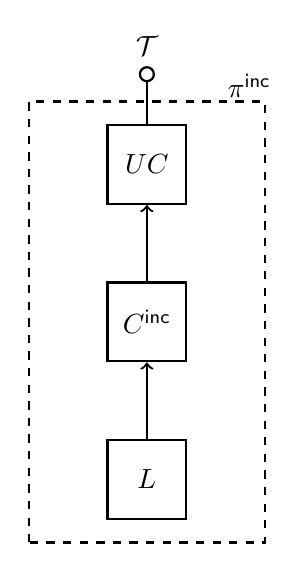
\begin{tikzpicture}[every path/.append style={draw, thick},rectangle/.style = {draw,minimum size=1cm}]
			\node (L)  at (0, 0) [rectangle]  {$L$};
			\node (Csmt)  at (0, 2) [rectangle]  {$C^\mathsf{inc}$};
			\draw      [->] (L) -- (Csmt);
			\node (UC) at (0, 4) [rectangle]   {$UC$};
			\draw      [->] (Csmt) -- (UC);
			\node (t)  at (0, 5.5)              {$\mathcal{T}$};
			\draw      [-o] (UC) -- (t);
			\draw[dashed] +(-1.5, -0.8) rectangle +(1.5, 4.8) +(1.3, 5) node {$\pi^\mathsf{inc}$};
		\end{tikzpicture}
		\caption{Inclusion Proof: SMT leaf $L$ with certificate chain through $UC$ to trust base $\mathcal{T}$} \label{fi:inc-proof}
	\end{minipage}
	\hfill
	\begin{minipage}[h]{0.45\linewidth}
		\centering
		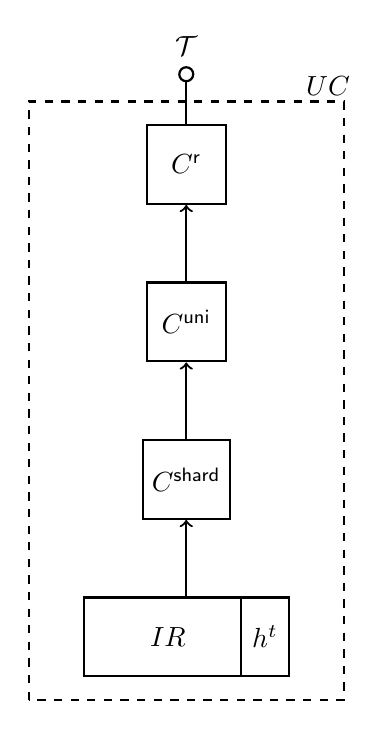
\begin{tikzpicture}[every path/.append style={draw, thick},rectangle/.style = {draw,minimum size=1cm}]
			\node (IR)  at (0, 0) [rectangle,minimum width=2.6cm]  {$IR$\ \ \ \ \ };
			\node (h)  at (1, 0) [rectangle,minimum width=.6cm]  {$h^t$};
			\node (Cs)  at (0, 2) [rectangle]  {$C^\mathsf{shard}$};
			\draw      [->] (IR) -- (Cs);
			\node (Cu) at (0, 4) [rectangle]   {$C^\mathsf{uni}$};
			\draw      [->] (Cs) -- (Cu);
			\node (Cr) at (0, 6) [rectangle]  {$C^\mathsf{r}$};
			\draw      [->] (Cu) -- (Cr);
			\node (t)  at (0, 7.5)              {$\mathcal{T}$};
			\draw      [-o] (Cr) -- (t);
			\draw[dashed] +(-2, -0.8) rectangle +(2, 6.8) +(1.8, 7) node {$UC$};
		\end{tikzpicture}
		\caption{Unicity Certificate is a chain of certificates and a certified input data record $IR$} \label{fi:uc}
	\end{minipage}
\end{figure}

See Fig.~\ref{fi:inc-proof} for the Inclusion Proof structure and Fig.~\ref{fi:uc} for the Unicity Certificate. The Inclusion Proof contains an SMT leaf $L = (\mathsf{sid}, \txhash)$ where $\mathsf{sid} = H(\predi, \sthash)$ is a state identifier and $\txhash$ is a transaction hash. The Inclusion Certificate $C^\mathsf{inc}$ connects the leaf to the SMT root hash $h$ in the Input Record. The Unicity Certificate then chains through the shard tree, unicity tree, and unicity seal to the global root of trust: Unicity Trust Base $\mathcal{T}$.


\subsection{Sparse Merkle Tree}\label{sec:smt}

\index{sparse merkle tree}\index{SMT}
The aggregation layer maintains a \emph{Sparse Merkle Tree} (SMT) in compressed paths form. The SMT maps state identifiers to transaction hashes and provides compact inclusion proofs. Refer to Appendix \ref{app:smt} for details.


\subsubsection{SMT Leaf Structure}

An SMT leaf contains a key-value pair:
\begin{itemize}
	\item \textbf{Key}: State identifier $\mathsf{sid} = H(\predi, \sthash)$ where:
	\begin{itemize}
		\item $\predi$ -- spending predicate of the token owner (Sec.~\ref{sec:predicates})
		\item $\sthash$ -- state hash representing the current state of a token
	\end{itemize}
	\item \textbf{Value}: Transaction data hash $\txhash$.
\end{itemize}

The SMT effectively maintains a mapping $\mathsf{sid} \mapsto \txhash$ that proves a state transition from state identifier $\mathsf{sid}$ was authorized via transaction with hash $\txhash$. This prevents double-spending: once a state identifier is registered in the SMT with a transaction hash, that state cannot be spent again.

\subsubsection{Inclusion Certificate}\label{InclusionCert}

\index{$C^\mathsf{inc}$ (Inclusion Certificate)}\index{Inclusion Certificate}
An \emph{Inclusion Certificate} $C^\mathsf{inc}$ for a leaf with key $\mathsf{sid}$ is a sequence of pairs:
\begin{equation*}
C^\mathsf{inc} = \langle (p_1, d_1), (p_2, d_2), \ldots, (p_n, d_n) \rangle
\end{equation*}
where each pair $(p_i, d_i)$ consists of:
\begin{itemize}
	\item $p_i \in \bitstr$ -- a path segment (bit-string)
	\item $d_i \in \hashtype \cup \bytes{\ast}$ -- for $i=1$ this is the leaf data, for $i>1$ this is a sibling hash value
\end{itemize}

The first pair $(p_1, d_1)$ contains the leaf's path segment and data. Each subsequent pair $(p_i, d_i)$ for $i > 1$ represents a step up the tree where $p_i$ is the path segment from the current node to its parent, and $d_i$ is the sibling hash value.

The concatenated path $p_1 \| p_2 \| \ldots \| p_n$ equals the full key $\mathsf{sid}$. The respective value $d_1$ records $\txhash$.

The verification function $\Call{smt\_verify\_inclusion}$ is provided in Appendix~\ref{sec:smt-verify-inclusion}.

\subsection{Shard Tree Certificate}\label{se:shard-tree-cert}

\emph{Shard Tree Certificate}\index{$C^\mathsf{shard}$ (shard tree certificate)}\index{shard tree certificate} connects the SMT root hash from a shard aggregator to a leaf of unicity tree. It is a tuple $C^\mathsf{shard} = (\sigma; h^s_1, \ldots, h^s_{|\sigma|})$, where:
\begin{enumerate}
	\item $\sigma=\sigma_1\sigma_2\ldots \sigma_{|\sigma|}$ is a shard identifier of type $\{0,1\}^\ast$
	\item $h^s_1, \ldots, h^s_{|\sigma|}$ -- sibling hashes of type $\hashtype$
\end{enumerate}

For the single shard case, the sharding scheme is $\{\emptystr\}$ and the certificate is $(\emptystr, \bot)$.

\subsubsection{Sharded SMT Structure}
% TODO: no hierarchy of aggregator nodes
In a sharded setting, each shard aggregator node maintains an SMT for its portion of the key space. The parent aggregator maintains a non-sparse tree (with all leaves present) where each leaf corresponds to a shard's SMT root hash.

To facilitate integration, each shard aggregator computes its root hash as $h_{\mathsf{root}} = H(p, h_L, h_R)$ where $p$ is a 1-bit path consisting of the leftmost bit of the shard identifier. This ensures the shard root hash can be directly used as a leaf value in the parent aggregator's tree.

\subsubsection{Creation: $\mathsf{CreateShardTreeCert}$}\label{se:create-shard-tree-cert}

\textbf{Input}:\index{functions!CreateShardTreeCert}
\begin{enumerate}
	\item $\sigma$ -- shard identifier
	\item $\chi$ -- shard tree of type $\chi \colon \overline{\mathcal{SH}}\to \hashtype$
\end{enumerate}

\textbf{Output}: shard tree certificate $C^\mathsf{shard}=(\sigma; h^s_1, \ldots , h^s_{|\sigma|})$

\textbf{Computation}:
\begin{algorithmic}
	\State $C \gets ()$
	\For{$i \gets  |\sigma|$ downto $1$}
		\State $C \gets C \mathbin{\|} \chi(\sigma_1\sigma_2\ldots\sigma_{i-1}\overline{\sigma_i})$
	\EndFor
	\State \Return $(\sigma; C)$
\end{algorithmic}

where $\sigma_1\sigma_2\ldots\sigma_m$ is the binary representation of $\sigma$, and $\overline{\sigma_i}$ is the binary complement of $\sigma_i$.

For the single shard case, the shard certificate is $(\emptystr,\bot)$.

\subsubsection{Computation: $\mathsf{CompShardTreeCert}$}\index{functions!CompShardTreeCert}

\textbf{Input}:
\begin{enumerate}
	\item $(\sigma;h^s_1, \ldots, h^s_{|\sigma|})$ -- shard tree certificate, where $\sigma=\sigma_1\sigma_2\ldots \sigma_{|\sigma|}$ is a shard identifier
	\item $IR$ -- Shard Input Record
	\item $h_t$ -- hash value of type $\hashtype$
\end{enumerate}
\textbf{Output}: Root hash $r$ of type $\hashtype$

\textbf{Computation}:

\begin{algorithmic}[0]
	\State $r \gets H(IR \mathbin{\|} h_t)$
	\For {$i \gets |\sigma|$ downto $1$ }
		\State \textbf{if} $\sigma_i = 0$ \textbf{then} $r \gets  H(r, h^s_i)$
		\State \textbf{if} $\sigma_i = 1$ \textbf{then} $r \gets  H(h^s_i, r)$
	\EndFor
	\State \Return $r$
\end{algorithmic}

For the single shard case, $\mathsf{CompShardTreeCert}((\emptystr, \bot), IR, h_t)$ returns $H(IR \mathbin{\|} h_t)$.

\subsection{Unicity Tree Certificate}\label{se:unicity-tree-certificate}

\emph{Unicity Tree Certificate}\index{$C^\mathsf{uni}$ (unicity tree certificate)}\index{unicity tree certificate} (Fig.~\ref{fi:uc}) is a tuple $C^\mathsf{uni} = (\beta, \mathsf{dhash}; (\beta_2, h_2), \ldots, (\beta_\ell, h_\ell))$, where:
\begin{enumerate}
	\item $\beta$ -- partition identifier of type $\mathbb{C}$
	\item $\mathsf{dhash}$ -- partition description hash of type $\hashtype$
	\item $(\beta_2, h_2), \ldots, (\beta_\ell, h_\ell)$ -- a sequence of partition identifier and sibling hash pairs
\end{enumerate}

\subsubsection{Creation: $\mathsf{CreateUnicityTreeCert}$}\label{se:create-unicity-tree-cert}\index{functions!CreateUnicityTreeCert}

\textbf{Input}:
\begin{enumerate}
	\item $\beta$ -- partition identifier of type $\mathbb{C}$
	\item $\mathcal{C}$ -- set of partition identifiers of type $\mathbb{C}$
	\item $\mathcal{CD}$ -- partition description of type $\mathbb{CD}[\mathcal{C}]$
	\item $\mathcal{IH}$ -- input hashes of type $\hashtype[\mathcal{C}]$
\end{enumerate}

\textbf{Output}: unicity tree certificate $(\beta, \mathsf{dhash}; (\beta_2, h_2), \ldots, (\beta_\ell, h_\ell))$

\textbf{Computation}:
\begin{algorithmic}
	\State $n \gets \len{\mathcal{C}}$ \Comment{Number of partitions}
	\State $C \gets \mathsf{sorted}(\mathcal{C})$ \Comment{Sorted list}
	\For{$i \gets 1 \ldots n$}
		\State $x_i \gets H(\mathcal{IH}[C_i] \mathbin{\|} H(\mathcal{CD}[C_i]))$
	\EndFor
	\State $\langle (\beta_1, h_1), (\beta_2, h_2), \ldots, (\beta_\ell, h_\ell) \rangle \gets \Call{\textsc{index\_tree\_chain}}{(C_1, x_1), (C_2, x_2), \ldots, (C_n, x_n), \beta}$ %\Comment{Sec.~\ref{sec:index-tree-chain}}
	\State \Return $(\beta, H(\mathcal{CD}[\beta]); (\beta_2, h_2), \ldots, (\beta_\ell, h_\ell))$ \Comment{Drop redundant first hash step}
\end{algorithmic}

\subsubsection{Computation: $\mathsf{CompUnicityTreeCert}$}
\index{unicity tree certificate!computation}
\textbf{Input}:
\begin{enumerate}
	\item $(\beta, \mathsf{dhash}; (\beta_2, h_2), \ldots, (\beta_\ell, h_\ell))$ -- unicity tree certificate
	\item $x$ -- input hash (output of the $\mathsf{CompShardTreeCert}$ function)
\end{enumerate}
\textbf{Output}: Root hash $r$ of type $\hashtype$

\textbf{Computation}:
\begin{algorithmic}[0]
	\State $L \gets \langle (\beta, H(x, \mathsf{dhash})), (\beta_2, h_2), \ldots, (\beta_\ell, h_\ell) \rangle$ \Comment{Restore the first hash step}
	\State \Return $\Call{\textsc{index\_tree\_output}}{L; \beta}$ \Comment{Sec.~\ref{sec:index-tree-output}}
\end{algorithmic}


\subsection{Unicity Seal}

\emph{Unicity Seal}\index{$C^\mathsf{r}$ (unicity seal)}\index{unicity seal} is a tuple $C^\mathsf{r} = (\alpha, n_r, e_r, t_r, r_-, r; s)$, where:
\begin{enumerate}
	\item $\alpha$ -- Network identifier
	\item $n_r$ -- BFT Core's Round number
	\item $e_r$ -- BFT Core's Epoch number
	\item $t_r$ -- Round creation time (wall clock value specified and verified by the BFT Core), with one-second precision. See Appendix~\ref{app:encodings} for encoding
	\item $r_-$ -- Root hash of previous round's Unicity Tree
	\item $r$ -- Root hash of the Unicity Tree (denoted as $r^{\text{root}}$ if necessary for clarity)
	\item $s$ -- Signature, computed by the BFT Core over preceding fields ($s = \mathsf{Sign}_{\mathsf{sk}_r}(n_r, e_r, t_r, r_-, r)$). The formulation of signature field depends on underlying consensus mechanism and its parameters. Here we assume an opaque data structure which can be verified based on the Unicity Trust Base, i.e., there is an implementation of an abstract function $\mathsf{Verify}_{\mathcal{T}}((n_r, e_r, t_r, r_-, r), s)$, encapsulated into the implementation of $\mathsf{VerifyUnicitySeal}$.
\end{enumerate}

$\mathsf{VerifyUnicitySeal}$ -- unicity seal verification function of type $\hashtype \times \mathbb{US} \times \mathbb{UB} \to \bool$\;. This function also verifies, if Unicity Seal's network identifier matches with the Unicity Trust Base.

\subsection{Unicity Certificate}\label{se:unicity-certificate}\index{$UC$ (unicity certificate)}

\emph{Unicity Certificate} is a tuple $UC = (IR, h_t, C^\mathsf{shard}, C^\mathsf{uni}, C^\mathsf{r})$, where:
\begin{enumerate}
    \item $\mathcal{IR}$ is a shard input record of type $\mathbb{IR}$ (Sec.~\ref{shard-input-record}),
    \item $h_t$ is the hash (of technical record) of type $\hashtype$,
    \item $C^\mathsf{shard}$ is a shard tree certificate,
    \item $C^\mathsf{uni}$ is a unicity tree certificate, and
    \item $C^\mathsf{r}$ is a unicity seal
\end{enumerate}

Elements of the tuple form an authenticated chain, see function \nameref{VerifyUnicityCert}.


\subsubsection{Verication: $\mathsf{VerifyUnicityCert}$}\label{VerifyUnicityCert}\index{functions!VerifyUnicityCert}

Verifies if unicity certificate is valid, based on unicity trust base as the root of trust.

\textbf{Input}:
\begin{enumerate}
	\item $UC = (IR, h_t, C^\mathsf{shard}, C^\mathsf{uni}, C^\mathsf{r})$ -- Unicity Certificate
	\item $\mathcal{T}$ -- Unicity Trust Base
\end{enumerate}

\textbf{Output}: \TRUE or \FALSE

\textbf{Computation}:

\begin{algorithmic}[0]
	\State $r\gets \mathsf{CompShardTreeCert}(UC.C^\mathsf{shard}, UC.IR, UC.h_t)$
	\State $r\gets \mathsf{CompUnicityTreeCert}(UC.C^\mathsf{uni}, r)$
	\State \Return $\mathsf{VerifyUnicitySeal}(r, C^\mathsf{r}, \mathcal{T}) = 1$
\end{algorithmic}


\section{Proofs}\label{se:proofs}

\subsection{Inclusion Proof}

\emph{Inclusion Proof}\index{$\pi^\mathsf{inc}$ (inclusion proof)}\index{inclusion proof} proves that a state transition (mapping from state identifier to transaction hash) has been registered in the SMT and certified by the BFT Core. It is a tuple $\pi^\mathsf{inc} = (L, C^\mathsf{inc}, UC)$, where:
\begin{enumerate}
	\item $L$ -- SMT leaf containing the state transition
	\item $C^\mathsf{inc}$ -- Inclusion Certificate (Sec.~\ref{InclusionCert})
	\item $UC$ -- unicity certificate (Sec.~\ref{se:unicity-certificate})
\end{enumerate}

\subsubsection{SMT Leaf}

An SMT leaf $L$ is a tuple $L = (\mathsf{sid}, \txhash)$, where:
\begin{itemize}
	\item $\mathsf{sid} = H(\predi, \sthash)$ -- state identifier, computed as the hash of the token owner's spending predicate and state hash
	\item $\txhash$ -- transaction data hash
\end{itemize}

SMT Leaf can be extracted from Inclusion Certificate like this:

\textbf{Input}: $C^\mathsf{inc} = \langle (p_1, d_1), (p_2, d_2), \ldots, (p_n, d_n) \rangle$ -- Inclusion Certificate

\textbf{Output}: $L = (\mathsf{sid}, h_{\mathsf{tx}})$ -- SMT Leaf

\textbf{Computation}:
\begin{algorithmic}[0]
	\State $\mathsf{sid} \gets p_1 \| p_2 \| \ldots \| p_n$ \Comment{Concatenate all path segments}
	\State $h_{\mathsf{tx}} \gets d_1$ \Comment{Extract leaf data from first pair}
	\State \Return $(\mathsf{sid}, h_{\mathsf{tx}})$
\end{algorithmic}

\subsubsection{Verification: $\mathsf{VerifyInclusionProof}$}\label{VerifyInclusionProof}\index{functions!VerifyInclusionProof}

$\mathsf{VerifyInclusionProof}$ -- inclusion proof verification function of type $\mathbb{IP} \times \mathbb{UB} \times \mathbb{CD} \to \bool$

\textbf{Input}:
\begin{enumerate}
	\item $\pi^\mathsf{inc} = (C^\mathsf{inc}, UC)$ -- inclusion proof
	\item $\mathcal{T}$ -- trust base
\end{enumerate}

\textbf{Output}: \TRUE or \FALSE

\textbf{Computation}:
\begin{algorithmic}[0]
	\State $h \gets UC.IR.h$ \Comment{Extract SMT root hash from IR}
	\If {$\neg \Call{smt\_verify\_inclusion}{\mathsf{sid}, h_{\mathsf{tx}}, C^\mathsf{inc}, h}$} \Return \FALSE \EndIf
	\If {$\neg \mathsf{VerifyUnicityCert}(UC, \mathcal{T})$} \Return \FALSE \EndIf
	\State \Return \TRUE
\end{algorithmic}

The inclusion proof applies to the leaf which matches the leaf extracted from the Inclusion Certificate.

\subsection{Non-Inclusion Proof}

\emph{Non-Inclusion Proof}\index{$\pi^\mathsf{exc}$ (non-inclusion proof)}\index{non-inclusion proof}\index{exclusion proof} proves that a state identifier does NOT exist in the SMT. It cryptographically demonstrates that a StateID is absent from the tree by showing the path to where it would be located if it existed.

A non-inclusion proof uses the same data structure as the inclusion proof but with different interpretation. The non-inclusion proof $\pi^\mathsf{exc} = (C^\mathsf{inc}, UC)$ of $\mathsf{sid}$ is valid if $\mathsf{VerifyInclusionProof}(\pi^\mathsf{exc}, \mathcal{T}) = \TRUE$ and $p_1$ is a prefix of $\mathsf{sid}$ and $d_1 = \emptyset$.


\subsection{Consistency Proof}\label{sec:consistency-proof}

\index{consistency proof}\index{$\pi_{CP}$ (consistency proof)}
A \emph{Consistency Proof} (also called \emph{non-deletion proof}) is a cryptographic construction that validates one round of operation of the append-only SMT maintained by aggregation layer nodes. It proves that the state transition from previous SMT root hash $h'$ to current SMT root hash $h$ was performed correctly: only new leaves were added, and no pre-existing leaves were removed or modified.

The consistency proof enables the BFT Core to verify the integrity of the Aggregation Layer's operations in a trustless manner.

For a batch of state transitions processed in a single round, the consistency proof $\pi_{CP}$ of type $\mathbb{CP}$ is a tuple $(B, \Pi)$ where $B$ is the batch of new SMT leaves and $\Pi$ contains the sibling hashes needed for verification (see Appendix~\ref{app:smt-consistency-proof} for detailed structure).

\subsubsection{Verification Function}\label{VerifyConsistencyProof}\index{functions!VerifyConsistencyProof}

$\mathsf{VerifyConsistencyProof}$ -- consistency proof verification function of type $\mathbb{CP} \times \hashtype \times \hashtype \to \bool$

\textbf{Input}:
\begin{enumerate}
	\item $\pi_{CP} = (B, \Pi)$ -- consistency proof where $B = \langle (\mathsf{sid}_1, h_{\mathsf{tx},1}), \ldots, (\mathsf{sid}_j, h_{\mathsf{tx},j}) \rangle$
	\item $h'$ -- previous SMT root hash (before the round)
	\item $h$ -- current SMT root hash (after the round)
\end{enumerate}

\textbf{Output}: \TRUE or \FALSE

The verification algorithm is defined in Appendix~\ref{sec:smt-verify-consistency-proof}.

A valid consistency proof guarantees: (1) \textbf{Append-only property}: No existing leaves were deleted or modified; (2) \textbf{Correctness}: All new leaves in batch $B$ were correctly inserted at positions determined by their state identifiers; (3) \textbf{Completeness}: The state transition from $h'$ to $h$ includes exactly the leaves in $B$ and no others.


%%%%%%%% BFT Core

\chapter{BFT Core}

\section{Data Structures of the BFT Core}

\subsection{Shard Input Record}\label{shard-input-record}

\emph{Shard input record} ($IR$)\index{$IR$ (input record)} of a shard of a partition (of type $\mathbb{IR}$) is a tuple $(n, e, h', h, t)$, where:
\begin{enumerate}
	\item $n$ -- shard's round number of type $\uint{64}$
	\item $e$ -- shard's epoch number of type $\uint{64}$
	\item $h'$ -- previous round's SMT root hash of type $\hashtype$
	\item $h$ -- current round's SMT root hash of type $\hashtype$
	\item $t$ -- reference time for request validation of type $\uint{64}$
\end{enumerate}

%The consistency proof $\pi_{CP}$ allows the BFT Core to verify that the state transition from $h'$ to $h$ was computed correctly by the aggregation layer nodes maintaining the SMT for this shard.

%Shard input record is created by the BFT Core in response to a certification request. The fields $n, e, h', h, v, h_B, f_B$ are copied from the certification request, and $h_t$ is added by the BFT Core.

%The field descriptions above apply to a committed (certified) Input Record. In the state certification \emph{request}, the fields are interpreted as follows: $h'$ - root hash to be extended (that is, of the last certified round), $h$, $v$, $h_B$ - values proposed for certification and $n$ is incremented for the proposed round.

\subsection{Statistical Record}\label{statistical-record}

Statistical record of type $\mathbb{SR}$ is a tuple $\mathsf{SR}=(n_e, \overline{\ell}_B, \overline{\ell}_S, \hat{\ell}_B, \hat{\ell}_S)$, where:\index{statistical record ($\mathsf{SR}$)}
\begin{enumerate}
	\item $n_e$ -- number of non-empty rounds (adding at least one new leaf), of type $\uint{64}$
	\item $\overline{\ell}_S$ -- memory usage of the SMT, of type $\uint{64}$
	\item $\hat{\ell}_B$ -- maximum number of SMT additions processed during a round, of type $\uint{64}$
\end{enumerate}

There is one Statistical Record of current epoch where the values are being updated, reflecting the current state since the beginning of the epoch; and one invariant Statistical Record of the preceding epoch of every shard of every public partition.

\subsection{Technical Record}\label{technical-record}

Technical record\index{technical record ($\mathbb{TE}$)} of type $\mathbb{TE}$ is a tuple $\mathsf{TE}=(n_r, e_r, \nu_\ell, h_\mathsf{sr})$, where:
\begin{enumerate}
	\item $n_r$ -- suggested next round number of type $\uint{64}$
	\item $e_r$ -- suggested next epoch number of type $\uint{64}$
	\item $\nu_\ell$ -- suggested leader identifier of type $\{0,1\}^\ast$
	\item $h_\mathsf{sr}$ -- hash of statistical records; type $\hashtype$
\end{enumerate}

Technical record is delivered with an Unicity Certificate. When a shard is extending the Unicity Certificate with a next round certification attempt, then it must use the suggested values provided in Technical Record.

There is one Technical Record for every shard of every partition, providing synchronization for the next round.

\subsection{Shard Info}

\emph{Shard info}\index{shard!shard info} of type $\mathbb{SI}$ is a tuple $(n, e, h_-, \mathsf{SR}_-, \mathsf{SR}, \mathcal{V}, \nu_\ell, UC_-)$, where:
\begin{enumerate}
	\item $n$ -- shard's round number of type $\uint{64}$
	\item $e$ -- shard's epoch number of type $\uint{64}$
	\item $h_-$ -- last-certified root hash
	\item $\mathsf{SR}_-$ -- statistical record of the previous epoch
	\item $\mathsf{SR}$ -- statistical record of the current epoch, initially (at each epoch) $(0,0,0,0,0)$
	\item $\mathcal{V}$ -- validators of the shard, a set of identifiers, each of type $\{0,1\}^\ast$
	\item $\nu_\ell$ --  leader identifier of type $\{0,1\}^\ast$ (it is assumed that $\nu_\ell\in \mathcal{V}$)
	\item $UC_-$ -- last created unicity certificate
\end{enumerate}

\subsection{Shard Tree}\label{se:shard-tree}

For a partition $\beta$, let $\mathcal{SH}_\beta = \mathcal{CD}[\beta].\mathcal{SH}$, and
$\mathcal{IRT}_\beta$ be of type $(\mathbb{IR},\hashtype)[\mathcal{SH}_\beta]$, i.e. for
every $\beta\in\mathcal{C}$ and $\sigma\in\mathcal{SH}_\beta$, $\mathcal{IRT}_\beta[\sigma]=(\mathcal{IR},h_t)$ (for some $\mathcal{IR}$ and $h_t$).

If there is no input from a shard to certify then $\mathcal{IRT}_\beta[\sigma] = \mathcal{IRT}_\beta[\sigma]_-$, that is, the value from the previously built Shard Tree is used. If there is no previous value then $\mathcal{IRT}_\beta[\sigma] = \zerohash$.

Shard tree\index{shard tree} for a partition $\beta$ is a function $\chi_\beta \colon \overline{\mathcal{SH}_\beta} \to \hashtype$ such that:
\begin{enumerate}
	\item If $\sigma\in\mathcal{SH}_\beta$, then $\chi_\beta(\sigma) = H(\mathcal{IRT}_\beta[\sigma]) =H(\mathcal{IRT}_\beta[\sigma].\mathcal{IR} \mathbin{\|} \mathcal{IRT}_\beta[\sigma].h_t)$.
	\item If $\sigma\in \overline{\mathcal{SH}_\beta}\backslash\mathcal{SH}_\beta$, then
		$\chi_\beta(\sigma) = H(\chi_\beta(\sigma\| 0)\, \mathbin{\|} \,\chi_\beta(\sigma\| 1))$.
\end{enumerate}
The value $\chi_\beta(\lfloor\!\rfloor)$ is called the root hash of the shard tree.

\emph{Shard tree certificate} for a shard $\sigma\in \mathcal{SH}_\beta$ is a sequence $h^s_1, \ldots, h^s_m$ of sibling hash values of type $\hashtype$, where $m=|\sigma|$ (the number of bits in $\sigma$); see Sec.~\ref{se:shard-tree-cert}.

\subsubsection{Shard Tree Creation: $\mathsf{CreateShardTree}$}\label{se:create-shard-tree}\index{functions!CreateShardTree}

\textbf{Input}:
\begin{enumerate}
	\item $\mathcal{SH}$ -- sharding scheme of type $\mathbb{SH}$
	\item $\mathcal{IRT}$ -- shard-specific data of type $(\mathbb{IR},\hashtype)[\mathbb{SH}]$
\end{enumerate}
\textbf{Output}: $\chi$ -- shard tree of type $\overline{\mathcal{SH}}\to \hashtype$

\textbf{Computation}:
$\chi\gets \bot$, $\mathsf{genST}(\emptystr)$

where $\mathsf{genST}$ is the following recursive function of type $\bitstr\to \hashtype$ with side effects:
\medskip

$\mathsf{genST}(\sigma)$:
\begin{enumerate}
	\item \textbf{if} $\sigma\in \mathcal{SH}$, \textbf{then store}  $\chi(\sigma) \gets H(\mathcal{IRT}[\sigma])$ and \textbf{return} $\chi(\sigma)$.
	\item\textbf{if} $\sigma\in \overline{\mathcal{SH}}\backslash\mathcal{SH}$, \textbf{then store}
		$\chi(\sigma) \gets H(\mathsf{genST}(\sigma\| 0) \mathbin{\|} \mathsf{genST}(\sigma\| 1))$ and \textbf{return} $\chi(\sigma)$
\end{enumerate}

For the single shard case, the shard tree is $\{(\emptystr, H(\mathcal{IRT}[\sigma])\}$, i.e. it only has a single record for the root hash $\chi(\emptystr)=H(\mathcal{IRT}[\sigma])$.

\subsection{Unicity Tree}\index{Unicity Tree}

Unicity Tree is an indexed Merkle tree that aggregates the state of all partitions in the network.

\subsubsection{Creation: $\mathsf{CreateUnicityTree}$}\label{se:create-unicity-tree}\index{functions!CreateUnicityTree}

\textbf{Input}:
\begin{enumerate}
	\item $\mathcal{C}$ -- set of partition identifiers of type $\mathbb{C}$
	\item $\mathcal{CD}$ -- partition description of type $\mathbb{CD}[\mathcal{C}]$
	\item $\mathcal{IH}$ -- input hashes of type $\hashtype[\mathcal{C}]$
\end{enumerate}
\textbf{Output}: $r$ -- unicity tree root hash of type $\hashtype$

\textbf{Computation}:
\begin{algorithmic}
	\State $n \gets \len{\mathcal{C}}$ \Comment{Number of partitions}
	\State $C \gets \mathsf{sorted}(\mathcal{C})$ \Comment{Sorted list}
	\For{$i \gets 1 \ldots n$}
		\State $x_i \gets H(\mathcal{IH}[C_i] \mathbin{\|} H(\mathcal{CD}[C_i]))$
	\EndFor
	\State \Return $\Call{\textsc{index\_tree\_root}}{(C_1, x_1), (C_2, x_2), \ldots, (C_n, x_n)}$ \Comment{Sec.~\ref{sec:index-tree-root}}
\end{algorithmic}

\section{State of the BFT Core}

\emph{State of the BFT Core}\index{BFT Core!BFT Core state} is a tuple $(\alpha, n, e, r_-, \mathcal{T}, \mathcal{C}, \mathcal{CD}, \mathcal{SI})$, where:
\begin{enumerate}
	\item $\alpha$ -- network identifier of type $\alpha$
	\item $n$ -- BFT Core's round number of type $\uint{64}$
	\item $e$ -- BFT Core's epoch number of type $\uint{64}$
	\item $r_-$ -- previous root hash of the unicity tree of type $\hashtype$
	\item $\mathcal{T}$ -- unicity trust base of type $\mathbb{UB}$
	\item $\mathcal{C}$ -- set of partition identifiers, with elements of type $\mathbb{C}$
	\item $\mathcal{CD}$ -- partition descriptions of type $\mathbb{CD}[\mathbb{C}]$
	\item $\mathcal{SI}$ -- shard info of type $\mathbb{SI}[\mathbb{C},\{0,1\}^\ast]$
\end{enumerate}

Epoch number\index{$e$ (epoch number)} can be interpreted as the version number of some shard's or BFT Core's configuration. It is used by supporting layers like orchestration and consensus. On static configuration, the epoch is $0$.

%Hash tree of the BFT Core (the unicity tree) is not considered as part of the state because it is created as a  per-round data-structure.

%In the implementation specification, additional datastructures are added to the state.
%For example, buffers may be needed for resending messages during communication error recovery, etc.

\section{Messages of the BFT Core}

\subsection{Certification Request}\label{certification-request}

\emph{Certification Request} (CR)\index{certification request (CR)} of a shard is a message $\langle \alpha, \beta, \sigma, \nu; \mathcal{IR}, \ell_B, \ell_S, [\pi_{CP}]; s; \rangle$, where:
\begin{enumerate}
	\item $\alpha$ -- network identifier of type $\mathbb{A}$
	\item $\beta$ -- partition identifier of type $\mathbb{C}$
	\item $\sigma$ -- shard identifier of type $\mathbb{SH}$
	\item $\nu$ -- validator identifier (aggregation layer node identifier) of type $\{0,1\}^\ast$
	\item $\mathcal{IR}$ -- shard input record of type $\mathbb{IR}$
	\item $\ell_B$ -- number of added new SMT leaves during the round, type $\uint{64}$
	\item $\ell_S$ -- SMT memory usage in bytes of type $\uint{64}$
	\item $\pi_{CP}$ -- consistency proof of type $\mathbb{CP}$ (Sec.~\ref{sec:consistency-proof})
	\item $s$ -- signature authenticating the message
\end{enumerate}

Certification requests are sent to the BFT Core by the aggregation layer nodes (validators) implementing the shards.

\subsection{Certification Response}\label{certification-response}

\emph{Certification Response} (CReS)\index{certification response (CReS)} of a shard is a message $\langle \alpha, \beta, \sigma, \mathsf{TE}; UC \rangle$, where:
\begin{enumerate}
	\item $\alpha$ -- network identifier of type $\mathbb{A}$
	\item $\beta$ -- partition identifier of type $\mathbb{C}$
	\item $\sigma$ -- shard identifier of type $\mathbb{SH}$
	\item $\mathsf{TE}$ -- technical record of type $\mathbb{TE}$
	\item $UC$ -- certified unicity certificate
\end{enumerate}

Certification response is sent by the BFT Core to the nodes of an aggregation layer nodes as a response to a certification request message. This is an asynchronous message: response is not immediate, and there can be multiple subsequent responses.

\section{Functional Description of the BFT Core}

\index{BFT Core!functional description}
During every round, the BFT Core receives certification requests from the shards of partitions
$\beta \in \mathcal{C}$.

The BFT Core certifies the SMT root hashes provided by the aggregation layer nodes. Each shard maintains an SMT for its portion of the key space. When aggregation layer nodes process Unicity Service Requests (as specified in Sec.~\ref{sec:request-validation}), they update their SMTs by setting leaves. The BFT Core certifies these updates by:
\begin{enumerate}
	\item Receiving certification requests containing the new SMT root hash $h$ and previous root hash $h'$
	\item Verifying the consistency proof $\pi_{CP}$ that proves correct SMT manipulation
	\item Certifying the new root hash via the Unicity Certificate
\end{enumerate}

As every shard $\sigma$ of a partition $\beta$ is implemented by a redundant distributed system with certain number $m=|\mathcal{SI}[\beta,\sigma].\mathcal{V}|$ of validator machines, it is possible that several certification requests $\mathsf{CR}_{\beta,\sigma}$ with the same $\mathsf{CR}_{\beta,\sigma}.\mathcal{IR}.h'$ but different $\mathsf{CR}_{\beta,\sigma}.\mathcal{IR}.h$ are received. This is solved by a majority voting mechanism requiring that
%\begin{enumerate}
%	\item
	a required majority, at least $\lfloor m/2\rfloor + 1$ of the dedicated validators, send $\mathsf{CR}_{\beta,\sigma}$ with an identical value of $\mathsf{CR}_{\beta,\sigma}.\mathcal{IR}.h$.
%	\item The leader $\mathcal{SI}[\beta,\sigma].\nu_\ell$ is in the majority
%\end{enumerate}
It is possible that not every shard sends its shard input record to the BFT Core during the round, and the majority voting may fail (see the Consensus specification for details).


For every incoming certificate request $\mathsf{CR}=\langle \alpha, \beta, \sigma, \nu; t, \mathcal{IR}, \ell_B, \ell_S\rangle$ the following checks are made
(if any of them fails, $\mathsf{CR}$ is discarded):
\begin{enumerate}
\item $\mathsf{CR}.\alpha = \alpha$ -- request came from the same network instance
\item $\mathsf{CR}.\beta\in \mathcal{C}$ and $\sigma\in \mathcal{CD}[\mathsf{CR}.\beta].\mathcal{SH}$ -- request came from a legitimate shard of a registered partition
\item $\mathsf{CR}.\nu\in \mathcal{SI}[\mathsf{CR}.\beta, \mathsf{CR}.\sigma].\mathcal{V}$ -- request came from an authorized aggregation layer node
\item $\mathsf{CR}.\mathcal{IR}.n=\mathcal{SI}[\beta,\sigma].n + 1$ -- round number is correctly incremented
\item $\mathsf{CR}.\mathcal{IR}.e=\mathcal{SI}[\beta,\sigma].e$ -- epoch number matches
\item $\mathsf{CR}.\mathcal{IR}.h'=\mathcal{SI}[\beta,\sigma].h_-$ -- previous round's SMT root hash in IR matches the recorded one
\item $\mathcal{CD}[\beta].\gamma_{CP}(\mathsf{CR}.\mathcal{IR}, \mathsf{CR}.\pi_{CP})$ -- consistency proof verification (Sec.~\ref{sec:consistency-proof}) succeeds: verify $\mathsf{VerifyConsistencyProof}(\mathsf{CR}.\pi_{CP}, \mathsf{CR}.\mathcal{IR}.h', \mathsf{CR}.\mathcal{IR}.h) = \TRUE$ and $|B| = \mathsf{CR}.\ell_B$ (batch size matches).
\item $\mathsf{CR}.\mathcal{IR}.t = \mathcal{SI}[\beta, \sigma].UC_-.IR.C^\mathsf{r}.t$ -- time reference is equal to the time field of the previous unicity seal
\end{enumerate}
Only one (majority-voted) certificate request (denoted by $\mathsf{CR}_{\beta,\sigma}$) is accepted from every shard.

When the BFT Core's round $n$ is completed, then:
\begin{enumerate}
	\item For every $\beta\in\mathcal{C}$, and $\sigma\in \mathcal{SH}_\beta$ with accepted certificate request \footnote{Please refer to the Consensus chapter for details; notably a ``request'' may be induced for technical reasons}:
	\begin{enumerate}
		\item $\mathcal{SI}[\beta, \sigma].n \gets \mathsf{CR}.\mathcal{IR}.n$
		\item $\mathcal{SI}[\beta, \sigma].h_- \gets \mathsf{CR}.\mathcal{IR}.h$
		\item $\mathcal{SI}[\beta, \sigma].\mathsf{SR}.n_e \gets \mathcal{SI}[\beta, \sigma].\mathsf{SR}.n_e + 1$
		\item $\mathcal{SI}[\beta, \sigma].\mathsf{SR}.\overline{\ell}_B \gets \mathcal{SI}[\beta, \sigma].\mathsf{SR}.\overline{\ell}_B + \mathsf{CR}.\mathcal{IR}.\ell_B$
		\item $\mathcal{SI}[\beta, \sigma].\mathsf{SR}.\overline{\ell}_S \gets \mathcal{SI}[\beta, \sigma].\mathsf{SR}.\overline{\ell}_S + \mathsf{CR}.\mathcal{IR}.\ell_S$
		\item $\mathcal{SI}[\beta, \sigma].\mathsf{SR}.\hat{\ell}_B \gets \max\{\mathcal{SI}[\beta, \sigma].\mathsf{SR}.\hat{\ell}_B, \mathsf{CR}.\mathcal{IR}.\ell_B\}$
		\item $\mathcal{SI}[\beta, \sigma].\mathsf{SR}.\hat{\ell}_S \gets \max\{\mathcal{SI}[\beta, \sigma].\mathsf{SR}.\hat{\ell}_S, \mathsf{CR}.\mathcal{IR}.\ell_S\}$
		\item The leader for next round: \\
			$\mathcal{SI}[\beta, \sigma].\nu_\ell \gets \Call{leaderfunc}{UC_-, \mathcal{SI}[\beta, \sigma].\mathcal{V}}$
		\item Technical record: \\
			$\mathcal{TE}_{\beta,\sigma} \gets (\mathcal{SI}[\beta,\sigma].n+1, \mathcal{SI}[\beta,\sigma].e, \mathcal{SI}[\beta,\sigma].\nu_\ell, h_\mathsf{sr})$ \;, \\
			where $h_\mathsf{sr}=H(\mathcal{SI}[\beta,\sigma].\mathsf{SR}_-, \mathcal{SI}[\beta,\sigma].\mathsf{SR})$
	\end{enumerate}

	\item For every registered partition $\beta\in\mathcal{C}$, the collected certification requests $\mathsf{CR}_{\beta,\sigma}$ are converted to a temporary data structure $\mathcal{IRT}_\beta$ of type $(\mathbb{IR},\hashtype)[\mathcal{SH}_\beta]$, where $\mathcal{SH}_\beta=\mathcal{CD}[\beta].\mathcal{SH}$,
	and $\mathcal{IRT}_\beta[\sigma]=(\mathsf{CR}_{\beta,\sigma}.\mathcal{IR}, H(\mathcal{TE}_{\beta,\sigma}))$; \\
	if there is no request then respective leaf repeats its previous value. If there is no previous value, the leaf is initialized to $\zerohash$.
	\item For every $\beta\in\mathcal{C}$, the shard tree $\chi_\beta$  (Sec.~\ref{se:shard-tree}) is created by the function call $\chi_\beta\gets\mathsf{CreateShardTree}(\mathcal{SH}_\beta,\mathcal{IRT}_\beta)$ (Sec.~\ref{se:create-shard-tree}).
	\item A temporary data structure $\mathcal{IH}$ of type $\hashtype[\mathcal{C}]$ is created such that $\mathcal{IH}[\beta]\gets \chi_\beta(\emptystr)$ for every $\beta\in\mathcal{C}$, i.e. $\mathcal{IH}$ contains the root hashes of the shard trees.
	\item The root of unicity tree is computed as $r \gets \mathsf{CreateUnicityTree}(\mathcal{C}, \mathcal{CD}, \mathcal{IH})$ (Sec.~\ref{se:create-unicity-tree})
	\item Unicity seal $C^\mathsf{r}=(\alpha, n, e, t, r_-,r; s )$ is created, where $t\gets\mathsf{time}()$ is the current time and $s$ is a "signature" on all other fields. The form of $s$ depends on the used consensus mechanism.
	\item For every $\beta\in\mathcal{C}$, the unicity tree certificate $C^\mathsf{uni}_\beta$ is created by the function call $C^\mathsf{uni}_\beta\gets \mathsf{CreateUnicityTreeCert}(\beta, \mathcal{C}, \mathcal{CD}, \mathcal{IH})$ (Sec.~\ref{se:create-unicity-tree-cert})
	\item For every $\beta\in\mathcal{C}$, and $\sigma\in \mathcal{SH}_\beta$:
	\begin{enumerate}
		\item The shard tree certificate $C^\mathsf{shard}_{\beta,\sigma}$ (Sec.~\ref{se:shard-tree-cert}) is created by the function call $C^\mathsf{shard}_{\beta,\sigma}\gets \mathsf{CreateShardTreeCert}(\sigma,\chi_\beta)$ (Sec.~\ref{se:create-shard-tree-cert})
		\item The unicity certificate $UC_{\beta,\sigma}=(\mathcal{IRT}_\beta[\sigma].\mathcal{IR},\mathcal{IRT}_\beta[\sigma].h_t, C^\mathsf{shard}_{\beta,\sigma}, C^\mathsf{uni}_\beta, C^\mathsf{r})$ (Sec.~\ref{se:unicity-certificate}) and the certification response $\mathsf{CReS}_{\beta,\sigma}=\langle \alpha,\beta,\sigma; UC_{\beta,\sigma}, \mathcal{TE}_{\beta,\sigma}\rangle$ are composed (if the shard input have changed)
		\item The last unicity certificate field is updated by $\mathcal{SI}[\beta,\sigma] UC_-\gets UC$ (if the shard input have changed).
	\end{enumerate}
	\item The round number and the previous root hash of the unicity tree are updated by $n\gets n+1$ and $r_-\gets r$.
\end{enumerate}

When a shard's (identified by $\beta$, $\sigma$) epoch with at least one non-empty round ends, the following assignments are executed:
\begin{enumerate}
	\item $\mathcal{SI}[\beta,\sigma].\mathsf{SR}_- \gets \mathcal{SI}[\beta,\sigma].\mathsf{SR}$
	\item $\mathcal{SI}[\beta,\sigma].\mathsf{SR} \gets (0,0,0,0,0)$
	\item $\mathcal{SI}[\beta,\sigma].e \gets \mathcal{SI}[\beta,\sigma].e + 1$
	\item The new validator set $\mathcal{SI}[\beta,\sigma].\mathcal{V}$ is chosen
\end{enumerate}


\chapter{Consensus Mechanisms}
\begin{leveldown}
  \chapter{Background}

\section{Definitions}\label{definitions}

\textbf{Block} is a set of requests, grouped together for mostly
efficiency reasons, to be processed during one round. Unicity BFT Core does not produce an explicit blockchain -- its certificates are persisted
as proofs within the tokens.

\textbf{UC} is \emph{Unicity Certificate}.

We call UC a \textbf{repeat UC}\index{repeat UC} if it has incremented round number for a particular
shard, but the certified hash has not changed compared to the UC of the previous round.

All aggregation layer nodes and BFT Core validators operate in \textbf{rounds}.

A round \textbf{extends} another finalized round by including its cryptographic
hash as the hash of previous round.

The validators of a shard are synchronized based on input
from the BFT Core. There are some fixed time-outs.

System has one BFT Core and an arbitrary number of
partitions, which may be split into arbitrary number of shards.

Within a shard, there are $k$ validators with identifier $\nu$, of which
$f$ might be faulty. For the BFT Core $k > 3f$. For a shard
$\sigma$, $k_{\beta, \sigma} > 2f$. We assume that all faulty validators may be
controlled by a coordinated, non-adaptive adversary. We assume trusted
setup (Genesis) and authenticated data links (signed messages). We assume
partially synchronous communication model where after unknown time GST
message delivery time is upper-bounded by known $\Delta$. We assume
that in every shard, at least one non-faulty validator is able to persist its
state.

A signature is denoted as $s$. Signed message with message name \texttt{name} is denoted as
$\langle \texttt{name} \mid a, b, c; s \rangle$.
Array of message fields is denoted as $\{f\}$.

Clients send \textbf{Unicity Service Requests} (requests).


\section{Scope}\label{scope}
Implementation details of BFT Core's atomic broadcast primitive (implementing the protocol
\texttt{Ordering}) are not given. This is a modular component. Only safety-critical validation rules are provided.


\section{Repeating Notation}\label{notation}

$n_r$ -- round number of the BFT Core\\
$n_{\beta, \sigma}$ -- round number of shard $\sigma$ of partition $\beta$\\
$k_{\beta, \sigma}$ -- number of aggregation layer nodes in shard $\sigma$ of partition $\beta$, $k_{\beta, \sigma} = |\mathcal{V}_{\beta, \sigma}| $\\
$\nu$ -- aggregation layer node identifier, unique within the Unicity System instance; set of a shard's nodes is $\mathcal{V} = \{\nu_i\}_{i\in \{1, \dots, k_\sigma\}}$ \\
$\nu_l \gets \Call{leaderfunc}{\cdot}$ -- leader identifier for this round \\
$h$ -- SMT root hash\\
$h'$ -- previous SMT root hash\\


$ensure(\ldots)$ -- function modeled after the Solidity language -- if its argument evaluates to true then nothing happens; if it evaluates to false then execution stops and function returns $0$. Unlike Solidity, should be complemented with returning and logging informative errors. Mostly used in message handlers for input validation. \\
$function(a, b \gets c)$ -- default value of function arguments, like in Python language. If 2nd argument is not specified by caller then parameter $b$ obtains the value of expression $c$.

\chapter{Aggregation Layer}\label{aggregation-layer}

\section{Timing}\label{HLCdetails-Timing}

An aggregation shard is synchronized using Input Records in returned UCs. For a shard, a UC can have
the following options:

\begin{enumerate}
\def\labelenumi{\arabic{enumi}.}
\item
  IR has not changed. Our shard can ignore this UC.
\item
  UC certifies an input from our shard, this input has never
  been certified before, and round number is incremented. This UC finalizes a round and starts a new round.
\item
  Round number is incremented, but state root hash remains the same (repeat UC). This UC starts another consensus attempt extending the same state as previous (likely failed) one.
  \item
  UC is newer, certifying a future state. Indicates to a validator that it is behind the others and must roll back the pending proposal and initiate recovery.
\end{enumerate}

If the latest UC certifies a state of this shard, then the certification response delivering UC
determines the leader and starts a new round.  While accepting incoming requests,
the leader starts assembling his next block proposal, extending the latest finalized round
(round with a valid UC).

When timer \texttt{t1} runs out the leader stops accepting new requests,
finishes state updates and broadcasts a block proposal to followers
and then sends Certification Request to the BFT Core. See Figure~\ref{fi:part-flow}.

BFT Core has a timer \texttt{t2} for every shard within every partition; it is reset when a valid
UC for this shard is issued. If this timer has run out, then a
\emph{repeat UC} is issued with incremented round number. This initiates a new consensus attempt for the shard. New round is executed with a different leader. Nodes
can determine which UC is the latest based on round number. A block proposal, generated by the leader, includes a UC and this UC must point to this leader. Round is finalized when its UC is embedded into the block. The retry mechanism is illustrated by Fig.~\ref{fi:part-exp-flow}.

\begin{figure}[!htbp]
	\begin{center}
		\includegraphics[width= 12cm]{pic/part-flow-ok.drawio.pdf}
		\caption{Successful Shard Round}\label{fi:part-flow}
	\end{center}
\end{figure}

\begin{figure}[!htbp]
	\begin{center}
		\includegraphics[width= 12.5cm]{pic/part-timing-exp.drawio.pdf}
		\caption{Shard Round attempt which did not produce a valid
    UC for this shard}\label{fi:part-exp-flow}
	\end{center}
\end{figure}



\section{Configuration and State}\label{configuration-and-state}

Configuration (managed by the Coordination Process) of every validator includes:

\begin{itemize}
\item
  Network Identifier ($\alpha$).
\item
  Partition Identifier ($\beta$).
\item
  Shard Identifier ($\sigma$); present for multi-shard partitions.
\item
  Aggregation Layer Node Identifier ($\nu$). There are $k_{\beta, \sigma}$ nodes in shard $\sigma$ of partition $\beta$.
\item
  Timeout value \texttt{t1}: after a node sees a UC which appoints a leader, the leader waits for \texttt{t1} time units before stopping accepting new Unicity Service Requests and creating a block proposal.
\end{itemize}

Communication layer:

\begin{itemize}
  \item secret key used to sign messages
  \item related public key; known to other validators and the BFT Core
  \item public keys of other validators within the shard
  \item communication addresses of other validators within the shard
  \item communication addresses of the BFT Core validators
\end{itemize}

Data layer:

\begin{itemize}
  \item Unicity \emph{Trust Base} ($\mathcal{T}$)
  \item other \emph{partition} defining parameters; refer to Unicity Platform Specification, State of a Shard.
\end{itemize}

\begin{algorithm}
  \caption{State and Initialization}\label{alg:init}
  \begin{algorithmic}[0]
    \State Constants:
    \State $\alpha$: Network Identifier
    \State $\beta$: Partition Identifier
    \State $\sigma$: Shard Identifier
    \State $\nu$: Node Identifier
    \State $k_{\beta, \sigma}$: number of nodes in the shard $\sigma$ of partition $\beta$
    \State $\mathcal{T}$: Unicity Trust Base, may \emph{evolve}
    \State Variables:
    \State $\nu_l \gets \NULL$: leader node identifier of the current round; $\NULL$ if not known
    \State $N \gets \{\}$: SMT (Sparse Merkle Tree)
    \State $\mathtt{cp} \gets \bot$: SMT Checkpoint
    \State $luc \gets \NULL$: latest valid UC
    \State $lte \gets \NULL$: latest technical record sent with latest UC
    \State                       \Comment{<\emph{round number to be certified}> $= lte.n$}
    \State                       \Comment{<\emph{last certified hash}> $= luc.IR.h$}
    \State $buf \gets \{\}$: input requests buffer
    \State $log \gets \{\}$: executed requests log for proposal creation
    \State $pr \gets \NULL$: pending proposal corresponding to a CR request waiting for UC
    \State $sr$: statistical record data. See \nameref{statistical-record}
    \State $\ell_B$: number of new SMT leaves added during round
    \State $\ell_S$: SMT memory usage in bytes
    \State $\pi_{CP}$: optional consistency proof (hash-based or ZK-compressed)
    \State $\mathcal{B}$: shared log
    \State
    \Function{start\_new\_round}{$uc, te$}
      \State ensure($\Call{VerifyUnicityCert}{uc, \mathcal{T}}$)
      \State ensure($uc.h_t = h(te)$)
      \State ensure($te.n > luc.IR.n$)
      \State ensure($uc.IR.h' = luc.IR.h$)   \Comment{Double-checking}
      \State $\mathtt{cp} \gets \Call{Checkpoint}{N}$
      \State \Call{RInit}{\null}
      \State $log \gets \{\}$
      \State $pr \gets \{\}$
      \State $\nu_l \gets te.\nu_l$
      \State $luc \gets uc, lte \gets te$
      \State \Call{reset\_timer}{$\mathtt{t1}$}
      \If{$\nu_l = \nu$}     \Comment{Leader}
        \State \Call{process}{$buf$}  \Comment{Process for no longer than until t1 tick}
        \State $buf \gets \{\}$
      \Else    \Comment{Follower}
        \If{$\Call{send\_InputForwardMsg}{l, buf}$}
          \State $buf \gets \{\}$  \Comment{Clean buffer on successful connection}
        \EndIf
      \EndIf
    \EndFunction
    \State
    \Function{leaderfunc}{$uc$}
      \State \Return $\{ \nu_i  \mid  i \gets \mathsf{integer}(H(uc)) \bmod k_{\beta,\sigma} + 1\}$  \Comment{Simplest example}
    \EndFunction
  \end{algorithmic}
\end{algorithm}

Variables:
\begin{itemize}
  \item $\nu_l$: Current round leader's identifier; $\NULL$ if not known
  \item $buf$: buffer with pending Unicity Service Requests
  \item $N$: State Tree
  \item $\mathtt{cp}$: State Tree checkpoint, helps the State Tree to roll back to previously certified state if a state extending attempt fails. Checkpoints can be released when a following round gets finalized.
  \item $luc$: latest UC. Importantly, this structure encapsulates the \emph{state hash} of the last certified state, to be extended by the round finalization attempt.
  \item $lte$: latest Technical Record, certified by $luc$. Carries the required \emph{round number}, leader identifier, epoch of the round finalization attempt.
  \item $log$: log of verified and executed (but not final) requests; respective changes in State Tree can be rolled  back by reverting it to checkpoint $\mathtt{cp}$.
  \item $pr$: Pending Certification Request waiting for UC; includes state tree hash and applied requests and round number as the time reference used for request validation. We are avoiding situation where there can be multiple pending requests and speculative validation; fresh UC invalidates all pending requests. \\
  There may be multiple parallel pending requests in future extensions.
  \item $\mathcal{B}$: the shared append-only log.
\end{itemize}

The variables are handled via state transitions like this:
\begin{enumerate}
  \item \emph{Initial state}. State tree is certified with `$luc$'; $log$ and $pr$ are empty; $\mathtt{cp}$ points to the current state.
  \item \emph{After applying any request(s)}: There are changes in the state tree; executed requests are recorded in $proposal$ (that is, $\mathtt{cp}$  is the starting point and $N$ and $log$ are updated in sync). Processing of requests continues.
  \item \emph{Waiting for UC}. This state is reached on \texttt{t1} click, after sending a BlockProposalMsg message (if being the leader) and sending a Certification Request. There are changes in the state tree on top of snapshot $\mathtt{cp}$; executed requests were recorded in $log$; Now, root hash of the state tree and respective $log$ are saved in $pr$, which extends $luc$. $pr$ must be preserved as long as it is possible that it gets certified by a UC. No new requests are processed in this state.
  \item \emph{After receiving a CReS message with new UC}:
  \begin{itemize}
    \item \emph{UC certifies $pr$}: block is finalized and added to $\mathcal{B}$. OK to clear.
    \item \emph{UC is `repeat UC'}: state is rolled back to $\mathtt{cp}$; we assume simplified case that consensus for prev. request is not possible any more and clean $pr$.
    \item \emph{UC certifies any round newer than the latest known UC}: rollback and recovery (independent state, consuming blocks until $N$ is up-to-date with UC).
    \end{itemize}
  \item Loop to 1.
\end{enumerate}

Please refer to Algorithm \ref{alg:init} for initialization.

\section{Subcomponents}\label{sub-components}

\begin{figure}[!htbp]
	\begin{center}
		\includegraphics[width=\textwidth]{pic/hlc-partition.drawio.pdf}
		\caption{Data Flow of the Shard Leader Node}
	\end{center}
\end{figure}


\subsection{Input Handling}\label{input-handling}

Input Handling prioritizes latency (fast finality). It is optimized for the case where there is enough processing capacity available and Unicity Service Requests do not have to be queued.

All validators accept Unicity Service Requests from clients. It is expected, that clients send Unicity Service Requests to many validators, as some may be byzantine. We assume that clients send Unicity Service Requests to the right shard; Unicity Service Requests sent to wrong shard can be discarded. Optionally, implement QoS / overload protection. There is no guarantee of execution -- the validators may drop Unicity Service Requests to protect the system availability, or when working close to maximum capacity. Synchronized clients may send Unicity Service Requests directly to the expected leader.

Shard validators forward Unicity Service Requests, as they arrive, to respective shard leaders (node producing the next block proposal); while observing time-outs and discarding expired Unicity Service Requests. There can be a light-weight partial validation, referred as \textit{sanity check}, before continuing with the processing. If the leader is not known, or rejects messages, then keep Unicity Service Requests in a buffer and try again when the next leader is known and accepts Unicity Service Requests. If the validator is the current leader, then he processes available Unicity Service Requests immediately. At the moment when a leader can not include transactions into a proposal anymore, or have collected enough transactions to fill a block, it starts rejecting incoming Unicity Service Requests from other validators.

A validator should retain a Unicity Service Request if accepted from a client or other validator; until it is either expired or included into a finalized block. A validator may forget a Unicity Service Request if accepted by another validator. A validator should not forward a Unicity Service Request to a distinct validator more than once.

Validators may limit the number of times a Unicity Service Request is forwarded.

Please refer to Algorithm \ref{alg:input} for an example without optional functionality.

\begin{algorithm}
  \caption{Input Handling}\label{alg:input}
  \begin{algorithmic}[0]
    \Message[TransactionMsg]{$Q$}
      \If{$\Call{sanity\_check}{Q}$}
         \If{$\nu_l = \nu$}                \Comment{This process is the leader}
           \State \Call{process}{$\{Q\}$}  \Comment{Beware of parallel execution}
         \ElsIf{$\nu_l \ne \NULL$}   \Comment{We know someone else is the leader}
           \If {$ \lnot \Call{send\_InputForwardMsg}{\nu_l, Q}$} \Comment{Forward to $\nu_l$}
             \State $buf \gets buf \cup Q$   \Comment{Store on failure}
           \EndIf
         \Else               \Comment{Buffer requests until leader is known}
           \State $buf \gets buf \cup Q$
         \EndIf
       \EndIf
    \EndMessage
    \State
    \Message[InputForwardMsg]{$reqs$}
      \If{$\nu_l = \nu$}                \Comment{This process is the leader}
        \State \textbf{defer} \Call{process}{$reqs$}
        \State \Return \textbf{``accepted''}
      \Else
        \State \Return \textbf{``reject''}
      %   \ForAll {$T \in txs$}
      %     \If{$\Call{sanity\_check}{T}$}
      %       \State $buf \gets buf \cup T$
      %     \EndIf
      %   \EndFor
      \EndIf
    \EndMessage
    \State
    \Event{next\_leader\_elected}
      \State \Call{prune\_expired}{$buf$}
      \If{$\nu_l = \nu$}                \Comment{This process is the leader}
        \State \Call{process}{$buf$}  \Comment{Beware of parallel execution}
      \Else
        \If {$\Call{send\_InputForwardMsg}{\nu_l, buf}$} \Comment{Forward to $\nu_l$}
          \State $buf \gets \{\}$   \Comment{Forget on successful send}
          \State   \Comment{\ldots or keep in ``forwarded'' buffer and use when becoming the leader}
       \EndIf
    \EndIf
    \EndEvent
  \end{algorithmic}
\end{algorithm}


\subsection{Block Proposal}\label{block-production}

\textbf{Summary}: On clock tick, stop immediate validation and execution of incoming Unicity Service Requests. Validate and execute Unicity Service Requests from the Request Buffer, updating the State Tree ($N$) and $log$ for proposal creation. Executed requests from $log$ go into Block Proposal, in the exactly same order they were validated and executed.
Broadcast Block Proposal to Follower Nodes. Create and send Uniqueness Certificate Request, retaining necessary state in a Pending Block Proposal ($pr$) data structure.

A round must extend a previously certified round. If a party approves a block proposal, then it also approves the entire history. This ensures safety of the protocol.

Pending Block Proposal ($pr$) must be stored in durable way before Certification Request can be sent, by e.g. writing it to persistent storage. Losing all copies of pending block proposals, while obtaining a UC for this round, would be an unrecoverable error.

\begin{algorithm}
  \caption{Producing a Block Proposal}\label{alg:proposal}
  \begin{algorithmic}[0]
    \Event{t1}
      \If{$\nu_l = \nu$}                \Comment{This validator is the leader}
        \State $\nu_l \gets \NULL$
        \State \Call{RCompl}{\null}  \Comment{Request processing must have stopped by now}
        \State $sr \gets \Call{ProduceStatistics}{\null}$
        \State \Call{send\_BlockProposalMsg}{$\alpha, \beta, \sigma, \nu, luc, lte, log, sr$} \Comment{Sign and Broadcast}
        \State \Call{do\_cert\_req}{$log, \nu, sr$}
      \EndIf
      \State $\nu_l \gets \NULL$          \Comment{Leader stops accepting new txs}
    \EndEvent
  \end{algorithmic}
\end{algorithm}

\begin{algorithm}
  \caption{Producing a Certification Request}\label{alg:ucrequest}
  \begin{algorithmic}[0]
    \Function{do\_cert\_req}{$txs, \nu_l, sr$}
      \State $h' \gets luc.IR.h$, $n \gets lte.n$, $e \gets lte.e$, $t \gets luc.C^\mathsf{r}.t$
      \State $h \gets \Call{StateRoot}{N}$
      \State $\ell_B \gets$ count of new SMT leaves added, $\ell_S \gets$ SMT memory usage
      \State $pr \gets (n, e, h', h, t, \nu_l, log, sr)$  \Comment{Pending Block Proposal}
      \If{\Call{store\_in\_durable\_way}{$pr$}}
        \State $IR \gets (n, e, h', h, t)$
        \State $\pi_{CP} \gets \Call{GenerateConsistencyProof}{h', h, \text{batch}}$ \Comment{Generate consistency proof}
        \State \Call{send\_CR}{$\alpha, \beta, \sigma, \nu, IR, \ell_B, \ell_S, \pi_{CP}$}
                 \Comment {Sign and send}
      \Else
        \State \Comment {Do nothing as the current node can not guarantee data availability}
        \State \Comment {The round may get finalized though thanks to other  partition nodes}
      \EndIf
    \EndFunction

    \Function{do\_cert\_req\_against}{$sr$}  \Comment{Voting against the proposal}
      \State $h' \gets luc.IR.h$, $n \gets lte.n$, $e \gets lte.e$, $t \gets luc.IR.C^\mathsf{r}.t$
      \State $h \gets \zerohash$
      \State $IR \gets (n, e, h', h, t)$
      \State $\ell_B \gets 0$, $\ell_S \gets 0$ \Comment{No additions when voting against}
      \State \Call{send\_CR}{$\alpha, \beta, \sigma, \nu, IR, \ell_B, \ell_S, \bot$}  \Comment{No consistency proof needed}
    \EndFunction
  \end{algorithmic}
\end{algorithm}

Please refer to Algorithm~\ref{alg:proposal} for details.

Note that a block can be without any requests; however, this does not necessarily imply $h' = h$, as system-initiated ``housekeeping'' actions may have changed the state.

\subsection{Validation and Execution}\label{validation-state-update}

\emph{Sanity checking} of Unicity Service Requests is quick and lightweight validation, with the main goal of protecting system resources by early detection of obvious garbage. All Unicity Service Requests will be fully verified later before actual execution. Thoroughness of sanity checking is a tuning parameter.

\emph{Validating} Unicity Service Requests is performing their full verification, according to Unicity Platform Specification, section \titleref{sec:request-validation}, and performing partition specific additional checks. The requests must appear in the \emph{proposal} in the same order. Requests without interdependencies (i.e., affecting distinct state) can be executed in parallel. Invalid requests are not executed and not included into produced proposal.

The expiration of Unicity Service Requests is checked relative to shard round number. Validation context includes also the time value $t$ obtained from previous UC and to be recorded as current round's $UC.IR.t$.

Refer to Algorithm~\ref{alg:execute} for details.

\begin{algorithm}[tb]
  \caption{Validate and Execute Unicity Service Requests}\label{alg:execute}
  \begin{algorithmic}[0]
    \Function{sanity\_check}{$Q; t \gets lte.n$}  \Comment{Requests will be fully validated later}
      \State \Return{ $Q.\mathsf{pk} \ne \NULL$}  \Comment{Basic validation of request structure}
    \EndFunction
    \State
    \Function{validate}{$Q; n \gets lte.n, t \gets luc.C^\mathsf{r}.t$}
      \State \Comment{Omitted, see Platform Specification, \titleref{sec:request-validation}}
    \EndFunction
    \State
    \Function{process}{$reqs$}   \Comment{Should be implemented as processing queue}
      \ForAll{$Q \in reqs$}
        \If{$\Call{validate}{Q}$}
          \State \Call{execute}{$N, Q$}   \Comment{Can be executed in parallel}
          \State $log \gets log \cup Q$
        \EndIf
      \EndFor
    \EndFunction
  \end{algorithmic}
\end{algorithm}


\subsection{Processing an Unicity Certificate and Finalizing a Round}\label{round-finalization}

\textbf{Summary:} On receiving a UC, round is finalized, and a new round is started.

More specifically,
\begin{enumerate}
  \item UC is verified cryptographically according to the Framework Specification. Partition and shard identifiers are checked.
  \item The time-stamp in UC is checked for sanity: it must not ``jump around'' and it must reasonably match the local time if it can be reliably determined. UC with a suspicious time-stamp must be logged, and processing continues because rejecting a UC may end with a deadlock of the shard.
  \item UC consistency is checked:
  \item UC is checked for equivocation, that is, for arbitrary $uc$ and $uc'$, the following must hold:
        \begin{align*}
        uc.IR.n = uc'.IR.n  \Rightarrow &\; uc.IR = uc'.IR \\
        uc.IR.h' = uc'.IR.h' \Rightarrow &\; uc.IR.h = uc'.IR.h\\
                            &\lor uc.IR.h' = uc.IR.h \lor uc'.IR.h' = uc'.IR.h\\
        uc.IR.h = uc'.IR.h \Rightarrow &\; uc.IR.h' = uc'.IR.h'  \\
                            &\lor uc.IR.h' = uc.IR.h \lor uc'.IR.h' = uc'.IR.h\\
        uc.IR.n = uc'.IR.n+1 \Rightarrow &\; uc.IR.h'  = uc'.IR.h\\
        uc.IR.n < uc'.IR.n \Rightarrow &\; uc.C^\mathsf{r}.n < uc'.C^\mathsf{r}.n
        \end{align*}
        On failing any of these checks, an equivocation proof must be logged with all necessary evidence.
  \item UC round number and epoch number can not decrement.
  \item On unexpected case where there is no pending round certification request, recovery is initiated, unless the state is already up-to-date with the UC.
  \item Alternatively, if UC certifies the pending round certification request then round is finalized.
  \item Alternatively, if UC certifies the round whose pending proposal tried to extend (`repeat UC') then state is rolled back to the previous state.
  \item Alternatively, recovery is initiated, after rollback. Note that recovery may end up with newer last known UC than the one being processed.
  \item Finally, on valid UC (validation reached the 3 alternatives above), a new round is started.
\end{enumerate}

Please refer to Algorithm~\ref{alg:ver-uc} for details. Round Finalization is presented in Algorithm~\ref{alg:finalize}.


\begin{algorithm}[tb]
  \caption{Processing a received Unicity Certificate}\label{alg:ver-uc}
  \begin{algorithmic}[0]
    \Message[CReS]{$\alpha, \beta, \sigma, te; UC$}
      \State ensure(\Call{VerifyUnicityCert}{$uc, \mathcal{T}$})
      \State ensure($H(te) = UC.h_t$)
      \If{ $\Call{got\_new\_uc}{UC}$ }
        \State $\Call{start\_new\_round}{UC, te}$
      \EndIf
    \EndMessage

    \Function{got\_new\_uc}{$uc$}
      \State ensure($uc.IR \ne luc.IR$)         \Comment{Ignore UC certifying the same}
      \State ensure($uc.C^\mathsf{r}.\alpha = \alpha$)
      \State ensure($uc.C^\mathsf{uni}.\beta = \beta$)
      \If{$\lnot$\Call{CheckSanity}{$uc.C^r.t, uc.C^r.n$, GetUTCDateTime()}}
          \State \Call{Log}{uc}  \Comment{Rejecting a UC with strange time would break the shard}
      \EndIf
      \State ensure(\Call{non\_equivocating\_ucs}{$uc, luc$})
      \State ensure($uc.IR.n > luc.IR.n$)  \Comment{Check late to catch equivocation}
      \If{$pr = \NULL$}  \Comment{No pending Certification Request}
        \If{$uc.IR.h \ne \Call{StateRoot}{N}$}
          \State \Call{recovery}{$uc$}
        \EndIf
      \Else
        \If{$uc.IR.h = pr.h \land uc.IR.h' = pr.h'$}
          \State \Call{finalize\_round}{$pr, uc$}
        \ElsIf{$uc.IR.h = pr.h'$}
          \State \Call{Revert}{$N, \mathtt{cp}$}
        \Else
          \State \Call{Revert}{$N, \mathtt{cp}$}
          \State \Call{recovery}{$uc$}
        \EndIf
      \EndIf
      \State \Return $1$
    \EndFunction
  \end{algorithmic}
\end{algorithm}


\begin{algorithm}
    \caption{Checking two UC-s for equivocation}\label{alg:malicious-uc}
    \begin{algorithmic}[0]
    \Function{non\_equivocating\_ucs}{$uc, uc'$}
      \State ensure($uc.IR.n \ge uc'.IR.n$)            \Comment{To simplify, assume that uc is not older than uc'}
      \State ensure($uc.C^\mathsf{r}.n_r > luc.C^\mathsf{r}.n_r$)
      \If{$uc.IR.n = uc'.IR.n$}
          \State ensure($uc.IR = uc'.IR$)              \Comment{On all failures log uc and uc' as proof}
      \EndIf
      \If{$uc.IR.h' = uc'.IR.h' \land uc'.IR.h' \ne uc'.IR.h$}
          \State ensure($uc.IR.h = uc'.IR.h$)          \Comment{A hash can be extended only with one hash}
      \EndIf
      \If{$uc.IR.h = uc'.IR.h$}                        \Comment{\ldots and vice versa}
          \State ensure($uc.IR.h' = uc'.IR.h'$)
      \EndIf
      \If{$uc.IR.n = uc'.IR.n + 1$}
          \State ensure($uc.IR.h' = uc'.IR.h$)
       \EndIf
      \State \Return $1$
    \EndFunction
  \end{algorithmic}
\end{algorithm}

\begin{algorithm}[tb]
  \caption{Finalizing a Round}\label{alg:finalize}
  \begin{algorithmic}[0]
    \Function{finalize\_round}{$pr, uc$}
      \State $\mathcal{B} \gets \mathcal{B} \cup (pr.txs; uc)$ \Comment{Recording a new batch to shard's log}
    \EndFunction
  \end{algorithmic}
\end{algorithm}

\emph{On arbitrary timeout} / \emph{lost connection}: re-establish connection to the BFT Core.

If a block can not be saved and made available during the finalization, then the round must be not closed. This ensures that a) the block can be restored based on saved proposal and UC during the recovery process, and b) the node can not extend the round with non-persisted block of inputs.


\subsection{Processing a Block Proposal}\label{block-input}

\begin{figure}[!htbp]
	\begin{center}
		\includegraphics[width=\textwidth]{pic/hlc-partition-follower.drawio.pdf}
		\caption{Data Flow of a non-leader aggregation shard node}\label{fi:part-follower}
	\end{center}
\end{figure}

\textbf{Summary:} Upon receiving a BlockProposalMsg message, create a rollback checkpoint and then validate the signature and header fields, execute Unicity Service Requests from the proposal and updating the State Tree ($N$). Executed requests go into Block Proposal. Create and send Uniqueness Certificate Request message, and retain a Pending Block Proposal data structure.

This procedure is performed by the non-leader validators. There are following steps (See Fig.~\ref{fi:part-follower}):

\begin{enumerate}
  \item Block proposal is checked: valid signature, correct partition and shard identifier, valid UC, the UC must be not older than the latest known by the validator. Sender must be the leader for the round started by included UC and match the leader identifier field.
  \item If included UC is newer than latest UC then the new UC is processed; this rolls back possible pending change in state tree. If new UC is `repeat UC' then update is reasonably fast; if recovery is necessary then likely it takes some time and there is no reason to finish the processing of current proposal.
  \item If the state tree root is not equal to one extended by the processed proposal then processing is aborted and negative vote is delivered.
  \item All Unicity Service Requests in proposal are validated; on encountering an invalid Unicity Service Request the processing is aborted and negative vote is delivered.
  \item Transaction orders are executed by applying them to the state.
  \item Pending certificate request data structure is created and persisted.
  \item Certificate Request query (CR) is assembled and sent to the BFT Core---that is, positive vote for the proposal.
\end{enumerate}

As an optimization, it is possible to vote against a proposal by sending a negative vote, where proposed state's hash is $\zerohash$. This helps the BFT Core to determine that convergence to consensus is not possible before waiting until time-out.

Please refer to Algorithm~\ref{alg:ver-proposal} for details.

\begin{algorithm}[tb]
  \caption{Processing a received Block Proposal}\label{alg:ver-proposal}
  \begin{algorithmic}[0]
    \Message[BlockProposalMsg]{$m = (\alpha, \beta, \sigma, \nu, uc, te, txs, sr; s)$}
      \State ensure(\Call{valid}{$m$})    \Comment{Consistent and authorized message}
      \State ensure(\Call{VerifyUnicityCert}{$uc, \mathsf{T}$})
      \State ensure($uc.h_t = h(te)$)
      \State ensure($m.\nu = te.\nu_l$)  \Comment{Signed by authorized leader}
      \State ensure($m.\alpha = \alpha \land m.\beta = \beta \land m.\sigma = \sigma$)
      \State ensure($m.te.n \ge lte.n$)
      \If{$\lnot\Call{CheckRequestStatistics}{sr}$}
        \State \Call{do\_cert\_req\_against}{$\NULL$}  \Comment{Invalid data, vote against}
        \State \Return
      \EndIf
      \If{$m.te.n > lte.n$}
         \State ensure($\Call{got\_new\_uc}{m.uc, m.te}$)  \Comment{Newer UC must be validated and processed}
         \If{\emph{processing of new UC took too much time (recovering?)}}
           \State \Return $\Call{start\_new\_round}{m.uc, m.te}$
         \Else
           \State $luc \gets m.uc, lte \gets m.te$
         \EndIf
      \EndIf
      \State $h' \gets m.uc.IR.h$
      \If{$\Call{StateRoot}{N} = h' \land \{\; \forall \; Q \in m.reqs \mid \Call{validate}{Q} \}$}
        \State $\mathtt{cp} \gets \Call{Checkpoint}{N}$
        \State \Call{RInit}{\null}
        \ForAll{$Q \in m.reqs$}
          \State \Call{execute}{$N, Q$}
        \EndFor
        \State \Call{RCompl}{\null}
        \State \Call{do\_cert\_req}{$m.reqs, m.\nu, sr$}  \Comment{Vote for}
      \Else
        \State \Call{do\_cert\_req\_against}{$sr$}  \Comment{Vote against}
      \EndIf
    \EndMessage
  \end{algorithmic}
\end{algorithm}

\subsection{Ledger Replication}\label{ledger-replication}

Relatively independent subsystem for serving and replicating ledger
data. Pseudocode of the service is provided in Algorithm~\ref{alg:replicate}.

\begin{algorithm}
  \caption{Ledger Replication}\label{alg:replicate}
  \begin{algorithmic}[0]
    \Message[LedgerReplication]{$\alpha, \beta, \sigma, n_1, n_2 \gets luc.IR.n; s$}
      \State \Comment{First authorization and sanity check,}
      \State \Return{$ \{ \mathcal{B}_{\alpha, \beta, \sigma, n} \mid n \in [n_1 \,.\,.\, n_2] \}$}
    \EndMessage
  \end{algorithmic}
\end{algorithm}

On receiving log, the blocks are verified using embedded UC-s and cryptographic links. See Platform Specification, function $\mathsf{VerifyBlock}()$.

\section{Recovery Procedure}\label{recovery-procedure}

If a validator is behind then it must use recovery procedure to sync its state with other validators, and obtain the latest UC for this shard, whose authoritative source is the BFT Core.

\textbf{Summary:} Missing log entries are fetched from other validators, validated, and applied to the state tree. A pending block proposal, if certified but not finalized, is applied and finalized.

\begin{figure}[!htbp]
	\begin{center}
		\includegraphics[width= 13cm]{pic/hlc-partition-recovery.drawio.pdf}
		\caption{Data Flow of an out-of-sync (recovering) Shard Node}
	\end{center}
\end{figure}

It is assumed that the state tree is already rolled back by calling $\Call{Revert}{N, \mathtt{cp}}$ if it had requests of a not finalized block applied.

In more details:
\begin{enumerate}
  \item Input UC is validated,
  \item Missing log entries are fetched from other (random) validator(s),
  \item Each request block is verified: cryptographically using embedded UC, and for correct partition and shard ID;
  \item Each request within the block is validated,
  \item Requests are applied to the state tree,
  \item Last known UC is updated if a block has newer one.
  \item Then, if there is a pending block proposal which can be finalized using freshly obtained UC then it will be applied to current state and round is finalized.
\end{enumerate}

Please refer to Algorithm~\ref{alg:recovery} for full details. Recursive recovery is used to mark locations where last-resort failover/retry happens. More intelligent failover and back-off mechanism could be used, with gracious shut-down on unrecoverable situations.

\begin{algorithm}
  \caption{Shard Node Recovery}\label{alg:recovery}
  \begin{algorithmic}[0]
    \Function{recovery}{$uc$}    \Comment{Assuming that Revert() is done by caller}
      \State ensure(\Call{VerifyUnicityCert}{$uc, \mathcal{T}$})
      \ForAll {$b \in \Call{send\_LedgerReplicationRequest}{luc.IR.n+1}$}  \Comment{To a random live validator}
        \If{$\Call{VerifyBlock}{b, \mathcal{T}}$}  \Comment{Assuming request blocks are ordered}
          \State ensure($b.\alpha = \alpha \land b.\beta = \beta \land b.\sigma = \sigma$)
           \State ensure($b.UC.IR.n > luc.IR.n$)
           \State ensure($\Call{StateRoot}{N} = luc.IR.h = b.IR.h'$)
           \State ensure($\{\; \forall \; T \in b.txs \mid \Call{validate}{T, luc.IR.n+1}\}$)
           \State $\mathtt{cp} \gets \Call{Checkpoint}{N}$
           \State \Call{RInit}{\null}
          \ForAll{$T \in b.txs$}
            \State \Call{execute}{$N, T$}
          \EndFor
          \State \Call{RCompl}{\null}
          \If{$\Call{StateRoot}{N} \ne b.IR.h$}
            \State \Call{Revert}{$N, \mathtt{cp}$}
            \State \Return \Call{recovery}{$uc$}  \Comment{Failover}
          \EndIf
          \State $\mathcal{B} \gets \mathcal{B} \cup b$
          \State $luc \gets b.UC$   \Comment{Respective $lte$ arrives with proposal}
        \Else
          \State \Return \Call{recovery}{$uc$}  \Comment{Failover}
        \EndIf
      \EndFor

      \If{$uc.IR.h' = \Call{StateRoot}{N}$} \Comment{Apply pending request if possible}
        \State $pr \gets \Call{fetch\_pr\_from\_persistent\_storage}{pr}$
        \If{$pr \ne \NULL \land pr.h' = uc.IR.h' \land pr.h = uc.IR.h$}
          \State ensure($uc.IR.n = pr.n$)
          \State ensure($\{\; \forall \; T \in pr.txs \mid \Call{validate}{T, pr.n} \}$)
          \State $\mathtt{cp} \gets \Call{Checkpoint}{N}$
          \State \Call{RInit}{\null}
          \ForAll{$T \in pr.txs$}
            \State \Call{execute}{$N, T$}
          \EndFor
          \State \Call{RCompl}{\null}
          \If{$\Call{StateRoot}{N} = uc.IR.h$}
            \State \Call{finalize\_block}{$pr, uc$}
            \State $luc \gets uc$
          \Else
            \State \Call{Revert}{$N, \mathtt{cp}$}
          \EndIf
        \EndIf
      \EndIf
    \EndFunction

  \end{algorithmic}
\end{algorithm}


\section{Protocols -- Shard Validators}\label{protocols-shard-nodes}

\subsection{Protocol TransactionMsg -- Unicity Service Request Delivery}\label{protocol-p0-transaction-order}

Users deliver their Unicity Service Requests to one or more validators (to account for byzantine validators censoring or re-ordering requests).

\textbf{Message}: $\langle \texttt{TransactionMsg} \mid Q\rangle$


\subsection{Protocol CR -- Round Certification Request}\label{protocol-p1-block-certification}

This section extends Sec.~\ref{certification-request}, \nameref{certification-request}).

If $h'$ is already `extended' with UC then the latest UC is returned
immediately via CReS message; otherwise validation and UC generation continues, UC is
returned via CReS when available.

If $h'$ is unknown to BFT Core then the latest UC is returned
immediately via CReS.

Returned message has a technical data record, which may trigger a view change: next consensus attempt with incremented round number and different leader.
An aggregation layer node can have only one pending CR per round number; subsequent messages are ignored. A message with higher round number is always preferred.

This message ``subscribes'' the validator to receive UC messages for a certain period, either a fixed number (e.g. $2$ rounds), or until the shard have successfully proposed a following round, that is, there is another set of BFT Core validators which have received a quorum of CR messages and therefore ``taken over'' the subscription.

\textbf{Message}: $\langle \texttt{CR} \mid \alpha, \beta, \sigma, \nu, IR, sr; s \rangle$

If an aggregation layer node has reasons to suspect that BFT Core have generated a new UC, then he must try to fetch it by trying again. $sr$ stands for \nameref{statistical-record}; a technical data structure sent from aggregation layer nodes to the BFT Core.

\subsection{Protocol RoundCertificationResponse (CReS)}

This section extends Sec.~\ref{certification-response}, \nameref{certification-response}).

CReS is asynchronous response (in the sense of data flow) to Certification Request (CR); there may be many CReS responses to one client request. $\mathsf{TE}$ stands for \nameref{technical-record}, sent from the BFT Core to aggregation layer nodes. Valid if $UC.h_t = h(\mathsf{TE})$.

Optional field RootTrustBaseEntry indicates, that UTB $\mathcal{T}$ have changed, e.g., have grown by the provided entry.

\textbf{Message}: $\langle \texttt{CReS} \mid \alpha, \beta, \sigma, UC, \mathsf{TE}, [\textsf{RootTrustBaseEntry}]\rangle$


\subsection{Protocol Subscription -- subscribing to CReS messages}

This message ``subscribes'' the validator to future CReS messages, without presenting a Certification Request in the form of CR message. Synchronous response is the latest UC for requestor.

Subscription ends when the shard have successfully proposed a following round, that is, there is another set of BFT Core validators which have received a quorum of CR messages and therefore serving a subscription.
% slower validators get UC with the next proposal

\textbf{Query}: $\langle \texttt{SubscriptionMsg} \mid \alpha, \beta, \sigma, \nu; s \rangle$

\textbf{Response}: $\langle \texttt{CReS} \rangle$


\subsection{Protocol InputForwardMsg -- Input Forwarding}\label{protocol-pc1-i-input-forwarding}

Forward a set of Unicity Service Requests.

\textbf{Message}: $\langle \texttt{InputForwardMsg} \mid \{Q\}\rangle$


\subsection{Protocol BlockProposalMsg -- Block Proposal}\label{protocol-pc1-o-block-proposal}

Leader broadcasts its input block proposal to other partition nodes.

\textbf{Message}: $\langle \texttt{BlockProposalMsg} \mid \alpha, \beta, \sigma, \nu_l, uc, te, txs, sr; s \rangle$ \\
where $txs = \{T\}$


\subsection{Protocol LedgerReplication -- Ledger Replication}\label{protocol-pc1-l-ledger-replication}

Let's assume that we have a separate layer of components implementing the
ledger storage. Entire ledger can be verified based on latest finalized and available
round and every block of inputs can be verified based on the Unicity Trust Base.

This protocol is provided by every functional aggregation layer node and dedicated \textit{archive nodes}; arbitrary parties can join the latter.

\textbf{Query}: $\langle \texttt{LedgerReplication} \mid (\alpha, \beta, \sigma n_1, [n_2] \rangle$

\textbf{Response}: $(\{B\})$

If 2nd number is missing then return everything till head. It is possible, that a reply misses some newer rounds, either because the queried node is behind or it prefers to return input blocks by smaller chunks.


\subsection{Protocol GetTrustBase -- Unicity Trust Base Distribution}\label{protocol-get-trust-base}

The Unicity Trust Base is a chain of records, one per epoch, containing the BFT Core validator set configuration and forming a verifiable root of trust. This protocol allows nodes to obtain Trust Base entries for a specified epoch range.

Each Trust Base entry corresponds to one epoch and contains validator identities, stakes, quorum requirements, and cryptographic linkage to the previous epoch's entry through hashing and signatures. The chain structure enables verification: given an authentic base entry, subsequent entries can be verified by checking signatures and hash chains.

Nodes request Trust Base entries by specifying an epoch range. The response includes all entries from the starting epoch up to (and including) the ending epoch, or up to the latest available entry if no ending epoch is specified.

\textbf{Query}: $\langle \texttt{GetTrustBase} \mid \alpha, e_1, [e_2] \rangle$

where:
\begin{itemize}
	\item $\alpha$ -- network identifier of type $\mathbb{A}$
	\item $e_1$ -- starting epoch number of type $\uint{64}$
	\item $[e_2]$ -- optional ending epoch number of type $\uint{64}$
\end{itemize}

\textbf{Response}: $\langle \texttt{TrustBaseResponse} \mid \mathcal{T} \rangle$

where $\mathcal{T} = \langle T_{e_1}, T_{e_1+1}, \ldots, T_{e_2} \rangle$ is a sequence of Trust Base entries.

Each Trust Base entry $T_e$ (for epoch $e$) is a tuple:
\[
T_e = (\alpha, e, n_e, \{\nu, b_\nu\}_e, k_e, r, h_{\mathsf{cr}}, h_{e-1}, s_{e-1})
\]
as defined in Table~\ref{ta:t-drc}.

If the ending epoch $e_2$ is omitted, the response includes all entries from $e_1$ up to the latest committed epoch. If the requesting node specifies an epoch range beyond what is currently available, the response includes entries up to the latest committed epoch only.

\textbf{Verification}: Upon receiving Trust Base entries, the requester must verify the chain:
\begin{enumerate}
	\item Verify that the first entry $T_{e_1}$ connects to an already-authenticated Trust Base entry (either the genesis entry or a previously verified entry)
	\item For each subsequent entry $T_{e_{i+1}}$, verify:
	\begin{enumerate}
		\item $h_{e_i} = H(T_{e_i})$ (hash chain linkage)
		\item Signature $s_{e_i}$ is valid over $T_{e_{i+1}}$ using validator set from epoch $e_i$
		\item Epoch numbers increment correctly: $T_{e_{i+1}}.e = T_{e_i}.e + 1$
	\end{enumerate}
\end{enumerate}

This protocol is provided by all active BFT Core validators. Validators maintain the complete Trust Base chain from genesis and serve requests for any epoch range. The protocol supports both initial synchronization (requesting from genesis) and incremental updates (requesting only recent epochs).


\chapter{BFT Core State Machine}\label{bft-core}

\section{Summary}\label{summary}

Leader-based BFT consensus based SMR. Roughly, BFT Core validators:

\begin{enumerate}
  \item
    Validate incoming Certification Requests: signature correctness, they must extend shard's previous UC, and partition specific checks must pass.
  \item
    Forward shard's requests to the BFT Core leader
  \item
    BFT Core leader verifies shard's requests (incl.~majority),
    produces UC tree, signs.
  \item
    BFT Core leader sends requests (all Certification Requests including
    signatures) and trees and signature to BFT Core validators.
  \item
    Followers verify shard's requests (incl.~majority), create trees,
    sign.
  \item
    Followers distribute their signatures to other BFT Core validators
  \item
    On reaching $k-f$ (there are $k$ validators in the BFT Core) unique
    signatures all BFT Core validators send \texttt{ack} to others
  \item
    On reaching $k-f$ \texttt{ack}-s all BFT Core validators commit and
    return responses to the aggregation layer nodes.
\end{enumerate}



\section{Timing}

BFT Core serves many partitions and shards, each implemented as a logical group of nodes. Operation cycles work like this:

\begin{enumerate}
  \item Shards operate in parallel:
  \begin{itemize}
    \item Shard validators send RoundCertificationRequest requests.
    \item Once there is a quorum of requests for a shard, the BFT Core updates an entry in the array of input records.
  \end{itemize}
  \item \emph{Eventually}, BFT Core starts Unicity Certificate generation. Fills data structure. Computes root. Signs. In distributed case this all takes some time.
  \item Individual tree certificates and UCs are generated for participating partitions. Responses are returned to individual validators.
\end{enumerate}

`Eventually' above is a compromise: 1) there is no sense to start a new round too fast, it is necessary to collect some input requests to certify; 2) input requests with quorum should be served as fast as possible to improve latency; 3) no need for further wait if all inputs are present; 4) some inputs might struggle with quorum; no need to wait for the long tail; 5) in order to generate `repeat UCs' a round must be restarted after \texttt{t2} time units even when there are no requests.

Configuration parameters are: target round rate $t_b$ and shard wait \texttt{t1}.\\
System parameters are: average root Certificate generation time  $t_r$;
average shard round processing time from receiving UC to sending Certification Request, including \texttt{t1} wait: $t_p$; with standard deviation $\sigma_p$. There are $k$ shards.

Let $m$ -- how many BFT Core rounds fit into one shard round; $m \approx (t_r + t_p) / t_b$.

Let's denote cumulative (normal) distribution of RoundCertificationRequest query messages with $\Phi_\sigma(x)$. Assume $m=1$, let's find a minimum of $(2-\Phi_\sigma(t_b - (t_r+t_p))(t_b)$ by adjusting $t_b$ and \texttt{t1}.

Practical rule for optimizing the average latency (Fig.~\ref{fi:root-timing}):\\
Start BFT Core round when completed quorum ratio is $t_b / \Delta \approx t_b / m(t_b - (t_r+t_p))$. Note that $t_b$ measures time from the moment when UC generation starts, thus it is circular and a rolling average must be used Median can be found by ignoring overflow from previous round and then waiting for completion of half of the quorums. Time from round start to next median is roughly $t_r+t_p$. Adjust \texttt{t1} if $t_b$ needs to be changed.

Even more practically:
\begin{enumerate}
  \item Maintain a rolling average of $t_b$ and $\Delta$
  \item Do not count the pending overflow from previous round
  \item After counting half of expected quorums ($k/2$) start timer for measuring $\Delta$ and re-start timer for measuring $t_b$
  \item After counting $k t_b / \Delta$ unique quorums stop timer $\Delta$ and start UC generation.
\end{enumerate}


\begin{figure}[!htbp]
	\begin{center}
		\includegraphics[width=\textwidth]{pic/root-timing.drawio.pdf}
		\caption{Optimal average latency is achieved when $\frac{A_1}{A_2} \approx \frac{t_b}{\Delta}$, where $A$ represents the respective area (number of messages). $t_b - \Delta \approx t_r+t_p$.}\label{fi:root-timing}
	\end{center}
\end{figure}

If the distribution gets too large it makes sense to increase $m$, that is, have more than one core round per one average shard's round.


\section{State}\label{root-state}

Please refer to Platform Configuration, State of the BFT Core, and Algorithm~\ref{alg:globals}.

Configuration is provided by the Governance and other management processes. State must be persisted and synchronized (recoverable from other BFT Core validators).

Time-outs and timers:
\begin{itemize}
\item
  \texttt{t2} -- BFT Core waits for \texttt{t2} time units before re-issuing a UC for a shard. This triggers a new round retrying certification of a block of inputs, with another leader. There is one timer instance per shard, referred as $\texttt{t2}_{\beta, \sigma}$ for the shard $\sigma$ of the partition $\beta$.
\item
  \texttt{t3} -- Triggers Unicity Tree re-calculation and UC response generation (monolithic BFT Core only);
  Target Round Rate ($t_b$) -- Distributed BFT Core specific parameter
\end{itemize}

Communication layer:
\begin{itemize}
  \item Validator's secret key used to sign its messages
  \item related public key; known to other BFT Core validators via the Governance Records, and to other parties via the $\mathcal{T}$
  \item public keys of other BFT Core validators (used by the underlying communication layer)
  \item public keys of Shard Validators (usage captured by the opaque function $\Call{valid}{\null}$)
  \item communication addresses of other BFT Core validators
  \item $conn[][]$ -- Connection contexts to return responses to validators which sent a RoundCertificationRequest request
\end{itemize}

\section{Analysis}

\subsection{Safety}
BFT Core enforces that each round is `extended' by one round only. This excludes conflicting rounds (forks). BFT Core must not generate ``equivocating'' UCs (see Section \ref{round-finalization} and Algorithm~\ref{alg:malicious-uc}).

\subsection{Liveness}
Usual properties of a partially synchronous communication model apply.

\subsection{Data Availability}
If a validator issues a RoundCertificationRequest call then it must not lose the block proposal (request data) until the block is finalized and committed to persistent storage.

The mechanism of `repeat UCs' presents a challenge: one block may receive multiple waves of extending attempts, initiated by subsequent `repeat UCs'. There are following options:
\begin{enumerate}
  \item Latest UC use is enforced strictly. If the BFT Core have issued a repeat UC, then all RoundCertificationRequest requests must be based on round number suggested by this response. Arriving and pending RoundCertificationRequest requests, referring to different round numbers, are dropped.
  \item All RoundCertificationRequest requests extending the current state are considered; if there is a pending request from a validator then it is replaced by later request from this validator, with larger round number.
  \item All RoundCertificationRequest requests extending the current state are considered, no matter the proposed round number, and included into pending request buffer; if one proposed new state achieves majority then it wins; this state does not have to be the latest one.
\end{enumerate}

On second and third option it is possible, that an aggregation layer node have issued multiple RoundCertificationRequest requests and eventually an older one gets certified. Thus, validators must retain all pending block proposals until one is committed.

These options provide somewhat better liveness of the protocol; in reality, if it is the case we can safely assume that time-out \texttt{t2} has too low value relative to system latencies. The rest of this specification assumes option 1.

Active aggregation layer nodes must retain their state until successfully---demonstrated by the ability to produce subsequent blocks---replaced by another set of validators after some epoch change. The long-term availability is provided by interested parties like RPC nodes, archive nodes, client middleware; these components must be able to replicate blocks with reasonable effort from the active validators.

\section{Monolithic Implementation}

\index{BFT Core!monolithic}
This section (Algorithms \ref{alg:globals}, \ref{alg:P1-req}, \ref{alg:uc-gen}) defines a monolithic, non-distributed BFT Core implementation. It serves distributed shards.

For a deployable implementation, please refer to Distributed BFT Core (Section~\ref{sec:distributed-bft-core}); it provides the same functionality to shards without being a single point of failure, and can provide necessary level of decentralization.

\begin{algorithm}
  \caption{Global Parameters and Variables}\label{alg:globals}
  \begin{algorithmic}[0]
    \State \emph{Configuration}:
    \State $\alpha$: Network Instance identifier
    \State $\mathcal{T}$: Unicity Trust Base
    \State $\mathcal{C}[]$: Partition Identifiers
    \State $\mathcal{CD}[]$: Partition Description Records
    \State \emph{State}:
    \State $n \gets 0$ : BFT Core's Round number
    \State $e \gets 0$ : BFT Core's Epoch number
    \State $r_- \gets \NULL$: Previous round's Unicity Tree root hash
    \State $\mathcal{SI}[][]$ - shard info of every $\sigma\in\mathcal{SH}_\beta$ of every $\beta\in\mathcal{C}$
    \State \emph{Variables}:
    \State $\forall \ \beta\in\mathcal{C}, \sigma\in\mathcal{SH}_\beta \colon \mathcal{IRT}_\beta[\sigma] \gets (\zerohash)$
    \State $\chi_\beta$: the shard tree for every $\beta\in\mathcal{C}$  (Sec.~\ref{se:shard-tree})
    \State $\upsilon$: unicity tree (Sec.~\ref{se:unicity-tree-certificate})
    \State $changes[][] \gets \bot$ Changes to IR, applied at the end of round, indexed by partition ID and shard number
    \State $req[][][] \gets \bot$: RoundCertificationRequest requests, indexed by partition ID, shard number and validator ID
    \State $conn[][][] \gets \bot$: Shard validator connections
    \State \emph{Timers}:
    \State $\Call{reset\_timer}{\texttt{t3}}$
    \State $\forall \ \beta\in\mathcal{C}, \ \forall \ \sigma\in\mathcal{SH}_\beta \colon  \Call{reset\_timer}{\texttt{t2}_{\beta, \sigma}}$
  \end{algorithmic}
\end{algorithm}


\subsection{Certification Request Processing}


Certification Request (CR) processing starts with sanity checking of the message. Then, checking if a newer UC is available; if yes then it is returned immediately. This would initiate shard recovery if necessary, and start a new shard round.

If a request tries to extend an unknown state, then the latest UC is returned immediately.

Next, the request is retained in request buffer if it is the first valid message; if the message is a repeating message then processing stops.

Equal requests (comparing entire IR to make sure that other fields also match) from the same shard are counted. If a request achieves simple majority then respective $IR$ gets added to the changes array waiting for certification, at position indexed by shard ID. If it is clear, that a shard can not converge to a majority agreement, then the slot in changes array is filled with $IR$ from the certified IR array, with incremented round number and previous certified hash set the same as the certified hash. This produces a `repeat UC' which, once delivered downstream, initiates a new shard consensus attempt.

See Algorithm~\ref{alg:P1-req}.

\begin{algorithm}
  \caption{CR Message Handling.}\label{alg:P1-req}
  \begin{algorithmic}[0]
    \Message[CR]{$m=(\alpha, \beta, \sigma, \nu, IR, \ell_B, \ell_S; s; [\pi_{CP}]); context$}
      \State ensure(\Call{valid}{$m$})
      \State ensure($m.\alpha = \alpha$)                           \Comment{Right network id}
      \State ensure($\beta \in \mathcal{C}$)                       \Comment{Valid part. id}
      \State ensure($\sigma \in \mathcal{CD}[\beta].\mathcal{SH}$) \Comment{Valid shard id}
      \State ensure($\nu \in \mathcal{SI}[\beta, \sigma].\mathcal{V}$) \Comment{Authorized validator}
      \State $conn[\beta][\sigma][\nu] \gets context$         \Comment{Network connection for returning messages}
      \If{$IR.n \ne \mathcal{SI}[\beta, \sigma].n+1$            \Comment{Round is behind/ahead}
        \State $\;\;\lor\; IR.e \ne \mathcal{SI}[\beta, \sigma].e$  \Comment{Epoch can be incremented by RP only}
        \State $\;\;\lor\; IR.h' \ne \mathcal{SI}[\beta, \sigma].h$ \Comment{Extending of unknown state}
        \State $\;\;\lor\; \lnot\mathcal{CD}[\beta].\gamma_{CP}(IR.h', IR.h, \ell_B, \pi_{CP})$  \Comment{Consistency proof verification}
        \State $\;\;\lor\; IR.t \ne \mathcal{SI}[\beta, \sigma].UC_-.C^\mathsf{r}.t$}   \Comment{Time not set as expected}
        \State \Call{send\_CReS}{$context; \beta, \sigma, \mathcal{SI}[\beta, \sigma].UC_-, \Call{get\_te}{\mathcal{SI}[\beta, \sigma]}$}
        \State \Return
      \EndIf
      \If{$req[\beta, \sigma][\nu]$}   \Comment{Reject duplicate request}
        \State \Return
      \EndIf
      \State ensure(\Call{tx-system-specific-checks}{$\mathcal{CD}[\beta], IR)$})
      \State $req[\beta, \sigma][\nu] \gets IR$  \Comment {Add the new message}
      \State $c \gets \max_{r \in req[\beta][\sigma]} \sum_{p \in  req[\beta][\sigma]}[r=p \land r.h \ne \zerohash]$  \Comment{Number of the max. matching votes,}
      \State    \Comment{Ignoring $\zerohash$, the ``negative vote''}
      \State $k \gets  |\mathcal{SI}[\beta, \sigma].\mathcal{V}|$ \Comment{Number of validators}
      \If{$c > k / 2 \land \lnot changes[\beta, \sigma]$}            \Comment{Consensus}
        \State $changes[\beta, \sigma] \gets \Call{certify}{IR, \mathcal{SI}[\beta, \sigma]}$
      \ElsIf{$\len{req[\beta, \sigma]} - c \ge k / 2$} \Comment{Consensus not possible}
        \State     \Comment{If max.match + |yet missing votes| < threshold }
        \State $changes[\beta, \sigma] \gets \Call{repeat\_cert}{\mathcal{SI}[\beta, \sigma]}$    \Comment{Produce `repeat UC'}
      \EndIf
    \EndMessage
  \end{algorithmic}
\end{algorithm}

\begin{algorithm}
  \caption{Certification helper functions}\label{alg:cert-helpers}
  \begin{algorithmic}[0]
    \Function{certify}{$ir:\mathbb{IR}, si:\mathbb{SI}$}
      \State $si \gets \Call{update\_shard\_info}{ir, si}$\Comment{Update caller's Shard Information record $si$}
      \State \Comment{According to Platform Specification, functional description of BFT Core}
      \State $te: \mathbb{TE} \gets \Call{get\_te}{si}$
      \State \Return $(ir, te)$
    \EndFunction

    \Function{repeat\_cert}{$si:\mathbb{SI}$}
      \State $si.n \gets si.n+1$  \Comment{Changing the parent's data structure as well}
      \State $si.\nu_l \gets \Call{leaderfunc}{si.UC_-, si.\mathcal{V}}$
      \State $rir: \mathbb{IR} \gets (si.UC_-.IR)$  \Comment{Repeat the previous UC's IR}
      \State $te: \mathbb{TE} \gets \Call{get\_te}{si}$
      \State \Return $(rir, te)$
    \EndFunction

    \Function{get\_te}{$si:\mathbb{SI}$}
      \State \Return $(si.n+1, si.e, si.\nu_l, h(si.\mathsf{SR}_-, si.\mathsf{SR}), h(si.\mathsf{VF}_-, si.\mathsf{VF}))$
    \EndFunction
  \end{algorithmic}
\end{algorithm}

\begin{algorithm}
  \caption{``SubscriptionMsg'' subscribes to UC feed}\label{alg:ping}
  \begin{algorithmic}[0]
    \Message[SubscriptionMsg]{$(\alpha, \beta, \sigma, \nu; s); context$}
      \State ensure(\Call{valid}{$(\alpha, \beta, \sigma, \nu; s)$})
      \State $conn[\beta, \sigma][\nu] \gets context$         \Comment{Network connection for returning subsequent messages}
      \State \Return $\Call{get\_uc}{\beta, \sigma}$
    \EndMessage
  \end{algorithmic}
\end{algorithm}

% \begin{algorithm}
%   \caption{``GetUCMsg'' returns the latest UC where $UC.IR.h \ne UC.IR.h'$}\label{alg:ping}
%   \begin{algorithmic}[0]
%     \Message[GetUCMsg]{$(\beta, \sigma; s); context$}
%       \State ensure(\Call{valid}{$(\beta, \sigma; s)$})
%       \State \Return $UC_\beta[\sigma]$
%     \EndMessage
%   \end{algorithmic}
% \end{algorithm}

\subsection{Unicity Certificate Generation}

Periodically, do the following:
\begin{enumerate}
  \item In case a shard has not shown progress for a period \texttt{t2} since the last UC was delivered then respective slot is  populated with the field content of previous certified IR array, with incremented round number. This produces a `repeat UC'.

  \item The pending changes in $changes$ array are applied to $IR$. If there are no new changes then the previous value is used.

  \item Based on the array of Shard Input Records, build the Shard Trees.

  \item Based on the roots of Shard Trees, build the Unicity Tree. Extract root hash value. Obtain wall clock time. Create the Unicity Certificate.

  \item For every record in IR changes array, respond to the shard based on request context from the request buffer. Then, clean up $req$ buffer, and reset respective \texttt{t2} timer.

  \item Finally, reset $changes$, update the previous root hash used for linking\footnote{Note that linear hash-linking using $r_-$  illustrates the idea that some sort of cryptographic linking is present; actual mechanism depends on the BFT Core implementation and used linking scheme.}, increment BFT Core round number and reset the timer $\mathtt{t3}$ which triggers the Unicity Certificate Generation (Algorithm~\ref{alg:uc-gen}).
\end{enumerate}

\begin{algorithm}
  \caption{Unicity Certificate Generation}\label{alg:uc-gen}
  \begin{algorithmic}[0]
    \Event{t3}  \Comment{Simplified, see section ``Timing''}
      \ForAll{$\beta \in \mathcal{C}$}   \Comment{Process partition timeouts}
        \ForAll{$\sigma \in \mathcal{SH}_\beta$}
          \If{$\lnot changes[\beta,\sigma] \land \Call{expired\_timer}{\texttt{t2}_{\beta, \sigma}}$}
            \State $changes[\beta,\sigma] \gets \Call{repeat\_cert}{\mathcal{SI}[\beta, \sigma]}$    \Comment{Produce `repeat UC'}
          \EndIf
        \EndFor
      \EndFor
      \ForAll{$(\beta, \sigma, ir, te) \in changes$}   \Comment{Apply changes}
         \State $\mathcal{IRT}_\beta[\sigma] \gets (ir, h(te))$
      \EndFor
      \ForAll{$\beta \in \mathcal{C}$}
        \State $\chi_\beta\gets\mathsf{CreateShardTree}(\mathcal{SH}_\beta,\mathcal{IRT}_\beta)$        \Comment{Sec.~\ref{se:create-shard-tree}}
        \State $\mathcal{IH}[\beta]\gets \chi_\beta(\emptystr)$
      \EndFor
      \State $r \gets \mathsf{CreateUnicityTree}(\mathcal{C}, \mathcal{CD}, \mathcal{IH})$ \Comment{Sec.~\ref{se:create-unicity-tree}}
      \State $t \gets \Call{GetUTCDateTime}$
      \State $C^\mathsf{r} \gets \Call{CreateUnicitySeal}{\alpha, n, e, t, r_-, r; \mathsf{sk}_r}$
      \ForAll{$(\beta, \sigma, ir, te) \in changes$}
        \State $req[\beta][\sigma] \gets []$
        \State $C^\mathsf{shard} \gets \Call{CreateShardTreeCert}{\sigma, \chi_\beta}$
        \State $C^\mathsf{uni} \gets \Call{CreateUnicityTreeCert}{\beta, \mathcal{C}, \mathcal{CD}, \mathcal{IH}}$
        \State $uc \gets (\mathcal{IRT}_\beta[\sigma].IR, \mathcal{IRT}_\beta[\sigma].h_t, C^\mathsf{shard}, C^\mathsf{uni}, C^\mathsf{r})$
        \State $\mathcal{SI}[\beta, \sigma].UC_- \gets uc$
        \ForAll{$connection \in conn[\beta][\sigma]$} \Comment{To all validators of the shard, in parallel}
          \State \Call{send\_CReS}{$connection; \alpha, \beta, \sigma, uc, te$} \Comment{Subscriptions expire -- see protocol desc.}
        \EndFor
        \State $\Call{reset\_timer}{\texttt{t2}_{\beta, \sigma}}$
      \EndFor
      \State $changes \gets \{\}$
      \State $r_- \gets r$
      \State $n \gets n+1$
      \State $\Call{reset\_timer}{\texttt{t3}}$
      \State \Comment{Note that $IRT$ retains its current value for the next round}
    \EndEvent
  \end{algorithmic}
\end{algorithm}


\section{Distributed Implementation}\label{sec:distributed-bft-core}

\index{BFT Core!distributed}
Distributed BFT Core is bisimilar to monolithic BFT Core in the sense that they provide the same service implementing the same business logic. Distributed BFT Core is Byzantine fault tolerant. It uses the SMR (State Machine Replication) concept.

\begin{figure}[htb]
	\begin{center}
		\begin{sequencediagram}
			\newthread{P1}{$\nu_1$}
			\newthread{P2}{$\nu_2$}
			\newinst[1]{R1}{$\nu^r_1$}
			\newinst{R2}{$\nu^r_l$}
			\begin{messcall}{P1}{\qquad CR}{R1}
        \begin{messcall}{P2}{CR}{R1}
          \begin{messcall}{R1}{\qquad IRChangeReq}{R2}
          \begin{sdblock}{atomic broadcast}{}
            \prelevel
            \mess{R2}{}{R1}
          \end{sdblock}
          \begin{call}{R1}{\!\!\!\!validation}{R1}{}
          \end{call}
          \prelevel\prelevel
          \begin{call}{R2}{\!\!\!\!validation}{R2}{}
          \end{call}
        \end{messcall}
        \prelevel
        \begin{messcall}{R1}{\qquad CReS}{P1}
        \end{messcall}
        \prelevel
        \mess{R1}{CReS}{P2}
      \end{messcall}
      \prelevel
    \end{messcall}
		\end{sequencediagram}
		\caption{Message flow (simplified)}\label{fi:rootflow}
	\end{center}
\end{figure}

The messaging between a shard and the BFT Core is illustrated by Figure~\ref{fi:rootflow}, where a shard with two validators $\nu_1$ and $\nu_2$ requests a UC. BFT Core is also depicted with two validators, the next leader after reaching a quorum of shard requests is $\nu^r_l$.

\subsection{Summary of Execution}

The summary follows the processing flow of a Certification Request by a BFT Core validator. The flow is illustrated in Fig.~\ref{fig:drc}; loosely moving counter-clockwise.

\begin{figure}[!htbp]
	\begin{center}
		\includegraphics[width=.8\textwidth]{pic/hlc-droot.drawio.pdf}
		\caption{Data-flow of a Distributed BFT Core Validator}\label{fig:drc}
	\end{center}
\end{figure}

\subsubsection{Peer Node Selection}

In order to use the distributed BFT Core, aggregation layer nodes must choose an appropriate subset of BFT Core validators to communicate with. The set must be shared by all aggregation shard nodes during one shard round; on receiving a ``repeat UC'', the validators must communicate with a different subset. The number of validators in this set is a tuning parameter: balances between availability and overhead. 2-3 validators is a good starting point. This number (in the sense of delivering messages in parallel) does not have security implications, as produced quorum sets retain aggregation layer nodes' signatures which can be verified independently. UC responses must be checked for equivocation.

If an aggregation layer node haven't received a UC-s from chosen BFT Core validators within $2 \times \texttt{t2}$ then it sends SubscriptionMsg requests to random other BFT Core validators. This ensures eventual synchronization if the firstly chosen validators happen to be faulty.

\subsubsection{CR Validation}

No difference from Monolithic Implementation, please refer to Algorithm~\ref{alg:P1-req} for details. If available, or on invalid request, UC is returned immediately by the same BFT Core validator.

\subsubsection{Shard Quorum Check}

Shard Quorum Check is the same as on Monolithic case (Alg.~\ref{alg:P1-req}). If a quorum is achieved or considered impossible, then a message is assembled (IRChangeReq), which includes all CR messages, and forwarded to the next BFT Core leader, using the Atomic Broadcast submodule.

\subsubsection{IR Change Request Validation}

The request must be validated analogously to the Algorithm~\ref{alg:ver-proposal}.

\subsubsection{Proposal Generation}

Leader collects all unique IR change requests and assembles the block proposal, which includes changed IR-s and a justification for each IR change request.
Next, if a particular IR has not been changed during \texttt{t2} timeout for this shard then the leader initiates ``repeat UC'' generation by including a specific record into the block proposal. There is no explicit justification, followers can validate timeouts based on their own timers.

In a proposal there can be up to one change request per shard.

Due to the pipe-lined finality, a proposal should not include IR change requests for slots with a valid IR change request in immediately preceding round. % should: proposal would be rejected, does not break anything.

Finally, the leader signs the proposal and broadcasts it to other BFT Core validators.

\subsubsection{Proposal Validation}

On receiving a proposal, validator validates it. There are consensus-specific checks. Every IR change request is validated based on its kind; base rules are presented by Algorithm~\ref{alg:ver-proposal}. Summary of the cases:

\begin{description}
  \item [Quorum achieved] The justification must prove the achievement of consensus by an aggregation shard. More than half of the shard nodes must have coherent votes.
  \item [Quorum not possible] The justification proves that there are enough conflicting votes to render the consensus impossible.
  \item [t2 timeout] The message states, that its timer have reached the timeout; all validators can confirm the timeout based on their own clocks, allowing a little drift.
\end{description}

After validating the proposal and checking the Voting Rule, the validator signs its vote data structure and sends it to the next leader in pipeline.

On encountering unexpected state hash the recovery process is initiated (see Section~\ref{root-recovery-procedure}).

\subsubsection{State Signing}

On assembling a Quorum Certificate (QC) with enough votes and verifying the Commit Rule the leader modifies state: for every newly certified IR element it updates its last UC array.

\subsubsection{UC Generation}

If a leader updates the last UC array element then it returns CReS responses to all pending aggregation shard nodes.

QC is included to HotStuff message pipeline, so it is broadcast to other validators (together with the new proposal produced by this validator). On seeing new QC and knowing re-certified IRs, other validators update their last UC arrays (the state).


\subsection{Proposal}

Proposal is a signed set of IR change requests, supplemented with proofs--the necessary number of signed partition nodes' messages (\textit{justification}). There are following options:
\begin{itemize}
  \item Change requests with justifications.
  \item Repeat Certification Request where consensus is considered impossible.
  \item Repeat Certification Request on \texttt{t2} timeout of a shard.
\end{itemize}


\subsubsection{State Synchronization}\label{root-recovery-procedure}

A BFT Core validator must have up-to-date vector of Input Records of all shards. There is no persistent blockchain. Returned Unicity Certificates, certifying IRs, are possibly persisted by the underlying layers.

The state includes necessary meta-data like the round number. This is provided by including the Unicity Seal, which also authenticates the IR vector.

State may include atomic broadcast module specific data, e.g. uncommitted round information.


\subsection{Atomic Broadcast Primitive}

The Atomic Broadcast primitive is instantiated using an adaptation of HotStuff consensus protocol. The adaptation is optimized towards better latency on good conditions. Therefore, a ``2-chain commit rule'' is used. Changes and tweaks wrt. the original HotStuff paper are:

\begin{itemize}
  \item ``2-chain commit rule''
  \item Timeout Certificates for view change. This induces quadratic communication complexity on faulty leader, but enables the 2-chain rule instead of 3-chain.
  \item QC component votes go to the next leader directly and the next leader assembles QC.
  \item Use of aggregated signatures (instead of threshold signatures)
\end{itemize}

More formally, critical elements of the operation of a HotStuff-derived algorithm are specified by the following rules.

Let $n$ denote round number, $B$ -- block of inputs, $QC$ -- Quorum Certificate, $TC$ -- Timeout Certificate.

\begin{ruledef}{Voting Rule} \\
  $B.n > $ last vote round \\
  $B.n = B.QC.n + 1 \lor (B.n = TC.n + 1 \land B.QC.n \ge max(\text{TC.tmo\_high\_qc\_round}))$
\end{ruledef}

\begin{ruledef}{Timeout Rule} \\
    $n \ge $ last vote round \\
    $(n = QC.n + 1 \lor n = TC.n + 1) \land QC.n \ge $ 1-chain round
\end{ruledef}

\begin{ruledef}{Commit Rule} \\
    It is safe to commit block $B$ if there exist a sequential 2-chain $B \leftarrow QC \leftarrow B' \leftarrow QC$ such that $B'.n = B.n + 1$.
\end{ruledef}

Please refer to the following papers for more details:

\begin{enumerate}
  \item \href{https://arxiv.org/abs/1803.05069}{HotStuff: BFT Consensus in the Lens of Blockchain}
  \item \href{https://developers.diem.com/papers/diem-consensus-state-machine-replication-in-the-diem-blockchain/2021-08-17.pdf}{DiemBFT v4: State Machine Replication in the Diem Blockchain}
\end{enumerate}

The concepts used in this specification map to the concepts used in the HotStuff and DiemBFT papers as follows:

\begin{description}
  \item[State:] Vector of Input Records
  \item[State Authenticator:] State is identified by the root hash of Unicity Tree.
  \item[Block Proposal:] List of changes to Input Records, with justifications; or a proposal to switch epochs.
  \item[Block:] There are no (explicit) blocks. The set of Input Records can be seen as the cumulative state after applying all previous (virtual) blocks. Unicity Certificates are propagated downstream to shards where they could be saved as part of shard blocks. Validator implementation is encouraged to produce an audit log with all the block proposal payloads.
  \item[Blockchain:] There is no such thing as the BFT Core Blockchain. However, Unicity Trust Base is somewhat blockchain-like: it gets a new entry added once per BFT Core epoch, and similarly to block headers, it can be interpreted as the Root of Trust.
\end{description}

\subsubsection{Round Pipeline}

Committing the payload happens across many rounds due to the pipe-lined nature of HotStuff. In consecutive rounds, the flow is like this:
\begin{enumerate}[nosep]
  \item vector of IR change requests (payload of the proposal message)
  \item updated IR-s (node block-tree) and Unicity Tree root (exec\_state\_id of a vote message)
  \item committed Unicity Tree Root (commit\_state\_id of a vote message).
\end{enumerate}

The output is commit\_state\_id from a Quorum Certificate which was formed by combining vote messages. QC is used to produce the Unicity Seal.

\subsubsection{Pacemaker}

Pacemaker is a module responsible for advancing rounds, thereby providing liveness. Pacemaker sees votes from other validators and processes local time-out event.

Pacemaker either advances rounds on seeing a QC from the leader or on no progress, on seeing a TC. On local timeout or seeing $f+1$ timeout messages a validator broadcasts signed TimeoutMsg message. TC is built from $2f+1$ distinct TimeoutMsg messages. All messages must apply to currently known HighestQC.

The BFT Core should not tick faster than configured Target Round Rate. In order to throttle the speed, there is deterministic wait performed by leaders at every round.

The wait must be reasonably small to not trigger TimeoutMsg messages from other validators.


\subsubsection{Leader Election}

Initially, a round-robin selection algorithm is used. In the roadmap there is stake weighted, unpredictable leader schedule.

Reputation is taken into account while producing per-epoch validator set assignments, for lowering the chance of inactive or unstable validator becoming a leader. One validator should not be the leader in two consecutive rounds.

Example: Take all validators. Remove one or more (fixed number) of the previous leaders. Remove all validators who did not participate in creation of the latest QC or TC. Pick one pseudo-randomly, and deterministically across all the validators, from the remainder.


\chapter{Dynamic System}

This section describes mechanisms making Unicity a dynamic system, by re-configuring partitions, shards and the BFT Core on the fly during execution. This introduces \emph{epochs}\index{epoch} -- time periods where the configuration is stable. Configuration changes are executed at the switch of epoch. Partitions, shards and the BFT Core are not synchronized with each other, they have independent rounds and epochs.

Also, the changing nature of some global data structures is discussed below.

\section{Configuration Changes}

Table~\ref{ta:when-epoch} provides a non-exhaustive list of configuration changes and the event synchronizing the change.

\begin{table}[!htbp]
	\begin{center}
		\caption{Synchronizing configuration changes.}\label{ta:when-epoch}
		\begin{tabular}{|p{0.7cm}|p{9cm}|p{2cm}|p{2.3cm}|}\hline
			No & Change                                     & RP epoch  & Shard epoch       \\\hline\hline
			1. & Adding, removing aggregation layer nodes          &        & \checkmark\\\hline
			2. & Adding, removing BFT Core validators & \checkmark &       \\\hline
			3. & Communication address change of validators &         &       \\\hline
			4. & Splitting (sharding) shards                &         & \checkmark \\\hline
			5. & Adding, removing partitions                &         & \checkmark \\\hline
			6. & RP's globally visible data structure changes (also increments versions of $\mathcal{T}$, $C^\mathtt{r}$, see Sec~\ref{sec:rp-versions})
                                                      & \checkmark & \\\hline
			7. & RP's operation rules          & \checkmark & \\\hline
			8. & Shard's data structure version changes resulting in changes in log content &         & \checkmark \\\hline
			9. & Shard's data structure version changes resulting in changes in proofs &         & \checkmark \\\hline
			10. & Changes in validation algorithms (ledger rules) &         & \checkmark      \\\hline

		\end{tabular}
	\end{center}
\end{table}

Adding and removing of validators may incur changes in the respective quorum sizes. Communication layer changes are entirely handled by the communication layer. By ``adding or removing a validator'' we mean a change in actively participating validator identifier sets.

\section{BFT Core Epoch Change}

In order to facilitate a dynamic, responsive BFT Core, it is necessary to adjust its parameters on the fly. In particular, it is necessary to add new validators and retire some existing ones to maintain a healthy validator set, due to changing requirements and operating conditions.

The configuration can be changed once per epoch. The source information comes from an Governance Process whose output is change records called Validator Assignment Records (Table~\ref{ta:var}).

Any BFT Core protocol leader can initiate an epoch change, given it has received the change record. The procedure works as follows:

\begin{enumerate}
  \item The leader produces a proposal where the usual payload is replaced by the Change Request justifying the increment of Epoch (Table~\ref{ta:rc-ecr});
  \item Validators who approve the epoch change continue with execution flow and do not include usual payload until the epoch change proposal gets committed.
  \item Next round after committing an epoch change is the first round of this epoch: Epoch in BlockData is incremented; and execution continues by the updated set of validators.
\end{enumerate}

\begin{table}[!htbp]
	\begin{center}
		\caption{BFT Core Epoch Change Request.}\label{ta:rc-ecr}
		\begin{tabular}{|p{0.5cm}|p{8cm}|p{1.7cm}|p{3.5cm}|}\hline
			No & Field                          & Notation  & Type                  \\\hline\hline
			1. & Epoch number                   & $e$       & $\uint{64}$           \\\hline
			2. & Validator identifiers and stakes& $\{\nu, b_\nu\}_e$ & $\{ (\bytestr, \uint{64}) \}$  \\\hline
			3. & Quorum size (Voting power)     & $k_e$     & $\uint{64}$           \\\hline
			4. & Hash of state summary          & $r$       & $\hashtype$          \\\hline
			5. & Hash of Change Record         & $h_{\mathsf{cr}}$ & $\hashtype$ \\\hline
			6. & Hash of the previous record    & $h_{e-1}$ & $\hashtype$          \\\hline
			7. & (attached) Change Record      &           & (Table~\ref{ta:var})  \\\hline
		\end{tabular}
	\end{center}
\end{table}

Fields 1, 2, 3 are copied from the Validator Assignment Records. The change record is a ``justification'': it is used as helper data for validators, but not included into the finalized record and resulting entry in the Unicity Trust Base. An implementation may choose to rely on alternative channels for distributing change records.

BFT Core's epoch change updates the Unicity Trust Base. On record-oriented Unicity Trust Base, the new record becomes part of Root Validator's state (see section~\ref{sec:ddrc}); and the new record gets propagated to Shard validators together with the next Unicity Certificate, as an extra field of the UCResp message.

\begin{ruledef*}{BFT Core Epoch Change} \\
  For every proof, the Epoch Number in its Unicity Certificate's Unicity Seal must point to the entry in Unicity Trust Base which can be used for this proof's verification.
\end{ruledef*}

Validators must not execute invalid change records and approve proposals with invalid Change Requests. Instead, the latest valid change record must be used, whenever available; skipping over of some if necessary.


\section{Shard Epoch Change}

Shard Epoch Change is triggered by the BFT Core, by incrementing the Epoch number field in Technical Record, returned with a UC.

The next shard round after finalizing a round with UC with incremented Epoch value is processed according to the configuration of the next epoch. Leader and validators are selected according to next epoch configuration.

\begin{ruledef*}{Shard Epoch Change} \\
  UC with incremented Epoch number in IR can be extended by a quorum of validators of the next epoch.
\end{ruledef*}

\section{Controlling Shard Epochs}

BFT Core triggers shard epoch changes. This happens in the following steps:

\begin{enumerate}
  \item BFT Core validators obtain the Change Record for the next epoch of a shard.
  \item If a BFT Core Leader includes an Input Record Change Request of a shard into a proposal and there is a pending epoch change of this shard, then the Change Record is included to the Request.
  \item Presence of Change Record is the signal that Epoch should be incremented. Included Change Record decision is validated, and if valid then epoch number in Technical Record (TE) is incremented. All other IR, TE changes are validated and applied as well.
  \item IR, TE-s get certified.
  \item New CReS message is returned to the shard.
  \item Shard's configuration is updated: quorum size (voting power needed for consensus), list of validators. This changes BFT Core's validation rules: the next Certification Request must be presented by a valid quorum of next epoch's aggregation shard nodes.
\end{enumerate}

\begin{ruledef*}{Shard Epoch Change Control} \\
  If a shard's state is certified by a UC with incremented Epoch number in certified TE, then the next shard round's requests get validated by the new epoch's configuration.
\end{ruledef*}

For the clarity of presentation, epoch handling is not present in the provided pseudocode. It supports the lower layer functionality of dynamic configuration changes.


\section{Validator's life cycle}

This section describes epoch changes from the viewpoint of an individual node, in particular, how a node joins and leaves shards.

Node accepts configuration updates through the Config API. The message is a set of change records, one per epoch. The records should cover the range from node's view of the current epoch to the epoch where node's status changes. The possible status changes (in respect to the current factual state of the node) are covered below.

It is assumed that the node have made itself already findable via the node discovery service.

\subsection{Shard Validator, joining} \label{sec:shard-node-joining}

Initially, a shard node is not an active validator. It receives a configuration message which indicates, that starting from epoch $e_{\beta, \sigma}$, this node is a validator in shard $\sigma$ of partition $\beta$. Following procedure is executed:

\begin{shaded}
  \begin{enumerate}[nosep]
    \item Reset \\
          Clean up state and storage, unless already synchronized to the required shard
    \item Start accepting proposals \\
          On incoming proposal message:
          \begin{itemize}[nosep]
            \item Extract the UC and update the last known UC if newer
          \end{itemize}
    \item Start accepting client requests \\
          On incoming client transaction:
          \begin{itemize}[nosep]
            \item If it is possible to determine the leader then forward client requests to the leader.
            \item Reject otherwise.
          \end{itemize}
    \item Obtain the latest UC for the shard $(\beta, \sigma)$ from the BFT Core.
    \item Launch recovery if behind
    \item Subscribe to log feed of the shard $(\beta, \sigma)$.\\
          On arrival of a new block of inputs:
          \begin{itemize}[nosep]
            \item Verify the inputs, apply the inputs to state and store in ledger
            \item If block's UC indicates that the expected epoch arrives:
            \begin{itemize}[nosep]
                \item Starting from the next round, this node is full validator
                \item Execution and message handling continues as a full validator
            \end{itemize}
          \end{itemize}
  \end{enumerate}
\end{shaded}

If the input block log streaming protocol is not available the procedure is as follows:

\begin{shaded}
  \begin{enumerate}[nosep]
    \item Reset \\
          Clean up state and storage, unless already synchronized to the required shard
    \item Start accepting proposals \\
          On incoming proposal message:
          \begin{itemize}[nosep]
            \item Extract the UC and update the last known UC if newer
          \end{itemize}
    \item Start accepting client requests \\
          On incoming client transaction:
          \begin{itemize}[nosep]
            \item If it is possible to determine the leader then forward client requests to the leader.
            \item Reject otherwise.
          \end{itemize}
    \item \textbf{loop:}
    \begin{itemize}[nosep]
      \item Obtain the latest UC from the BFT Core
      \item Launch recovery if the node is behind
      \item If the UC indicates that the epoch where node is a full validator have started:
      \begin{itemize}[nosep]
        \item this node is now a full validator,
        \item exit loop.
      \end{itemize}
    \end{itemize}
  \end{enumerate}
\end{shaded}

The state graph is depicted at Figure~\ref{fi:node-state-graph}.

\begin{figure}[!htbp]
	\begin{center}
    \begin{tikzpicture}[node distance=3cm]
      \tikzset{every node/.append style={font=\tiny}}
      \node[state, initial, accepting] (q1)  {free};
      \node[state, right of=q1] (q2) {staked};
      \node[state, right of=q2] (q3) {pooled};
      \node[state, right of=q3] (q4) {assigned};
      \node[state, right of=q4] (q5) {active};
      \path[->] (q1) edge [bend left] node [above]  {staking proof} (q2)
                (q2) edge [bend left] node [below]  {unstaking tx}  (q1)
                (q2) edge             node [above]  {joining tx}    (q3)
                (q3) edge             node [below, label={[align=left]change \\ record}] {} (q4)
                (q4) edge             node [below, label={[align=left]joining \\ epoch}] {} (q5)
                     edge [loop above] node         {synchronize} ()
                (q5) edge [loop above, dashed] node {unassign tx} ()
                     edge [bend left] node [above]  {leaving epoch} (q2);
    \end{tikzpicture}
    \caption{Node state graph (node's view)}\label{fi:node-state-graph}
  \end{center}
\end{figure}

\subsection{Shard Node, leaving}

If the node is an active validator and it receives indication that from an epoch $e$ this node is not any more a member of shard $(\beta, \sigma)$, then the following procedure is executed:

\begin{shaded}
  On receiving a UC indicating the expected epoch update:
  \begin{enumerate}[nosep]
    \item Starting from the next round, this node is not a validator.
    \item Stop accepting proposals.
    \item Stop accepting client request messages.
    \item OK to reset the state.
    \item Continue serving the log replication protocol; it is mandatory to retain the storage until the next quorum have committed at least one round.
    \item OK to reset the log.
  \end{enumerate}
\end{shaded}

The node (more specifically the node operator) can initiate the leaving process by sending an ``unassign transaction'' to the Governance Body. Processing may take arbitrary time, and the unassignment may happen for other reasons as well. Validators are encouraged to not drop off without executing the unassignment process.

Now, the node may submit a request to the Governance Body to be assigned again as an active node, possibly at another shard. The node is encouraged to keep its identity.

\begin{ruledef*}
  Every Shard Node must ensure the availability of generated ledger until the next validator set takes over.
\end{ruledef*}

\subsection{Shard Node, ambiguous records}

If there is a double assignment before leaving then the validator must continue at the current shard. When eventually the validator gets dismissed, it must join according to the latest valid change record.


\subsection{BFT Core Node, joining}

\begin{shaded}
  On receiving a change record:
  \begin{enumerate}[nosep]
    \item Obtain the current BFT Core configuration via the GetUnicityTrustBase RPC call
    \item Validate the updated Unicity Trust Base
    \item Make itself findable via the node discovery service
    \item Start listening to BFT Core proposal messages.\\
          On receiving a proposal where ProposalMsg.BlockData.Epoch is incremented and the epoch includes the node:
          \begin{itemize}[nosep]
            \item Use the BFT Core recovery protocol (GetStateMsg / StateMsg) to synchronize the state,
            \item Process the proposal,
            \item Start processing shard Certification Requests,
            \item Continue as full BFT Core validator.
          \end{itemize}
  \end{enumerate}
\end{shaded}

\subsection{BFT Core Node, leaving}

A BFT Core node may leave the active validator set after performing a successful epoch change, where this node is not a member of the new validator set anymore. The node is responsible for successful hand-over: by making its state available to the new joining nodes briefly after the beginning of the next epoch, and offering the Unicity Trust Base distribution service without limitations to all current and near-future validators.

A BFT Core node (more specifically, the operator of the node) can initiate the leaving process by sending a specific ``unassign transaction'' to the Governance Body. Processing may take arbitrary time, and the unassignment may happen for other reasons as well. BFT Core validators are strongly encouraged to not drop off without executing the unassignment process.

\begin{ruledef*}
  BFT Core Node must keep running until the next epoch's Unicity Trust Base entry gets committed.
\end{ruledef*}


\section{Dynamic Data Structures}

\subsection{Versioning}\label{sec:rp-versions}

The content of Unicity Seal and Unicity Trust Base\index{$\mathcal{T}$ (unicity trust base)}, globally used data structures across the Unicity Platform, depend on Distributed BFT Core implementation details. These data structures must be versioned to accommodate necessary iterative changes while the BFT Core implementation roadmap is being executed. That is, $\mathcal{T} = (v, \cdot)$ and $C^\mathsf{r} = (v, \cdot)$, where $v$ is the version number and the rest depends on the version. In the following sections, we assume that a section shares the same version number and it is omitted for brevity.

Accordingly, the function $\mathsf{VerifyUnicitySeal}$ must be able to verify a recent subset of Unicity Seal versions, based on an authentic copy of the up-to-date Unicity Trust Base. This can be imagined as a wrapper, where the version number of input chooses the right implementation.

\subsection{Evolving}

Unicity Trust Base itself evolves (e.g., new records are added, while format/version stays the same) when the BFT Core validator set changes. Every evolved copy of Unicity Trust Base is cryptographically verifiable based on an older authentic copy of the Unicity Trust Base.

We denote the initial, authentic\footnote{Authenticity is guaranteed by e.g., off-band verification of the Genesis Block and embedding the newest possible Unicity Trust Base into the verifier code during release management process, analogously to \emph{certificate pinning}.} Unicity Trust Base as $\mathcal{T}_\mathsf{base}$ and updated Unicity Trust Base as $\mathcal{T}$, and for each version of data structures define the function

\[ \mathsf{VerifyUnicityTrustBase}_{\mathcal{T}_\mathsf{base}}(\mathcal{T})  \; .
  \]

For every supported version of proofs an implementation of $\mathsf{VerifyUnicitySeal}$ and the relevant Trust Base must be provided. Only the latest version of Unicity Trust Base can evolve.

At the launch, the system is bootstrapped to a genesis state where the content of Unicity Trust Base, together with Genesis Blocks, are created via some off-chain social consensus process. The relevant data structures are the same, while references to previous states and signatures created by previous states are hard-coded to zero values.


\subsection{Monolithic, Static BFT Core}

We start with one BFT Core validator, which does not change (and can not change its keys).

\begin{itemize}
  \item $\mathcal{T} = (\alpha, \mathsf{pk})$\,, \\
  where $\alpha$ is the system identifier and $\mathsf{pk}$ is the public key of the BFT Core.
  \item $C^\mathsf{r} = (\alpha, n_r, t_r, r_-, r; s)$\,, \\
  as defined in the Platform Specification; $s$ is a digital signature created using BFT Core's secret key.
\end{itemize}

\begin{algorithmic}[0]
  \Function{VerifyUnicitySeal}{$r, C^\mathsf{r}, \mathcal{T}$}
    \State \Return $(\mathcal{T}.\alpha = C^\mathsf{r}.\alpha \land r = C^\mathsf{r}.r  \land \mathsf{Ver}_{\mathcal{T}.\mathsf{pk}}(C^\mathsf{r}, C^\mathsf{r}.s))$  \Comment{Calculated over all fields except signature}
  \EndFunction
\end{algorithmic}

\begin{algorithmic}[0]
  \Function{VerifyUnicityTrustBase}{$\mathcal{T}_\mathsf{base}, \mathcal{T}$}
    \State \Return $(\mathcal{T}_\mathsf{base} = \mathcal{T})$  \Comment{No changes are allowed}
  \EndFunction
\end{algorithmic}


\subsection{Monolithic, Dynamic BFT Core}\label{ch:m-rc}

In the case of dynamic BFT Core the validator(s) can change at epoch boundaries. The identifier (public key) of new validator is signed by the current one, and this signed record is appended to the Unicity Trust Base.

\begin{itemize}
  \item $T_e = (\alpha, e, \mathsf{pk}_e; s)$ \\
  is Unicity Trust Base Record, where $s = \mathsf{Sig}_{\mathsf{sk}_{e-1}}(T_e)$ is a cryptographic signature over verification record of epoch $e$ (calculated over all fields except signature), signed by the previous epoch's secret key of the BFT Core.
  \item $\mathcal{T} = (T_j, T_{j+1}, \ldots, T_k)$\,, \\
  where $j$ is the first epoch and $k$ is the latest epoch covered. In the pseudocode below, we use notation $\mathcal{T}[j] := (T \in \mathcal{T}\colon \; T.e = j )$, that is, the element pointing to the epoch number $j$. System instance identifier of every epoch is invariant: $\forall\ i, j \colon T_i.\alpha = T_j.\alpha$.
  \item $C^\mathsf{r} = (\alpha, n_r, t_r, r_-, r; (s, e))$  \\
  as defined in the Platform Specification; $s$ is a cryptographic signature created using BFT Core's secret key of the epoch $e$.
\end{itemize}

\begin{algorithmic}[0]
  \Function{VerifyUnicitySeal}{$r, C^\mathsf{r}, \mathcal{T}$}
    \If{$(\mathcal{T}.\alpha \ne C^\mathsf{r}.\alpha \lor r \ne C^\mathsf{r}.r$}
        \State \Return $0$
    \EndIf
    \If{$\mathcal{T}[C^\mathsf{r}.e] = \bot$}
      \State \Return \textbf{error}  \Comment{No record in trust base for the epoch}
    \EndIf
    \State \Return $(\mathsf{Ver}_{T.\mathsf{pk}}(C^\mathsf{r}, C^\mathsf{r}.s) = 1)$  \Comment{Calculated over all fields except signature}
  \EndFunction
\end{algorithmic}

Note that the caller must ensure that a relevant record is present in Unicity Trust Base, that is, $\mathcal{T}[C^\mathsf{r}.e] \ne \bot$. Obtaining a fresh Unicity Trust Base is covered by the Chapter Unicity Anterior.

\begin{algorithmic}[0]
  \Function{VerifyUnicityTrustBase}{$\mathcal{T}_\mathsf{base}, \mathcal{T}$}

    \State $bmax = \max_{T \in \mathcal{T}_\mathsf{base}} T.e$  \Comment{Last epoch in trust base}
    \State $tmin = \min_{T \in \mathcal{T}} T.e$ \Comment{First epoch number to be verified}
    \If{$tmin > bmax+1$}
        \State \Return \textbf{error}  \Comment{Not a continuous chain}
    \EndIf
    \For{$T \in \mathcal{T}$}
       \If {$\mathcal{T}_\mathsf{base}[bmax].\alpha \ne T.\alpha$}
          \State \Return \textbf{error}  \Comment{Non-invariant system id}
       \EndIf
    \EndFor
    \For{$j \in \{tmin \,.\,.\,bmax+1\}$}   \Comment{Verify based on available trust base}
       \If{ $\mathsf{Ver}_{\mathcal{T}_\mathsf{base}[j-1].\mathsf{pk}}(\mathcal{T}[j], \mathcal{T}[j].s) = 0$}
          \State \Return $0$
       \EndIf
    \EndFor
    \For{$j \in \{tmin+1 \,.\,.\,\max_{T \in \mathcal{T}} T.e\}$} \Comment{Verify consistency of new}
       \If{ $\mathsf{Ver}_{\mathcal{T}[j-1].\mathsf{pk}}(\mathcal{T}[j], \mathcal{T}[j].s) = 0 $}
          \State \Return $0$
       \EndIf
    \EndFor
    \State \Return $1$
  \EndFunction
\end{algorithmic}

For efficiency, the user must cache the verification results. For example: 1) at the startup, the bundled trust base is checked for consistency, and 2) each time an evolved trust base is encountered, a) it is checked for equivocation, b) if the trust base is newer than the base and verified using the function $\mathsf{VerifyTrustBase}$, then the base trust base is updated with new records from the new trust base (or substituted with the latest version if the implementation is accumulator-like).

This version is illustrative and not for implementation.


\subsection{Distributed, Static BFT Core}

Unicity Trust Base is a map of BFT Core validator identifiers to validator public keys, and a number $q$ which specifies the required quorum size, i.e.,
\begin{itemize}
    \item $\mathcal{T} = (\alpha, \{ (i, \mathsf{pk}_i)  \mid i \gets 1 \ldots \nu_r  \}, q) \quad\text{ where }\quad q \ge \nu_r - f \,,$
    \item $C^\mathsf{r} = (\alpha, n_r, t_r, r_-, r; s) \quad \text{where} \quad s = \{(i, s_i) \mid i \in (1 \,.\,.\, \nu_r)  \}  \quad \text{and} \quad \lvert s \rvert \ge q$\,. \\
\end{itemize}

Unicity Trust Base does not change as the BFT Core configuration is static.

\begin{algorithmic}[0]
  \Function{VerifyUnicitySeal}{$r, C^\mathsf{r}, \mathcal{T}$}
    \If{$\mathcal{T}.\alpha \ne C^\mathsf{r}.\alpha \lor r \ne C^\mathsf{r}.r$}
        \State \Return $0$
    \EndIf
    \If{$\lnot ( \forall\ m, n \in 1 \,.\,.\, \lvert C^\mathsf{r}.s \rvert \colon C^\mathsf{r}.s[m].i \ne C^\mathsf{r}.s[n].i )$}
      \State \Return 0 \Comment{Duplicate signers}
    \EndIf
    \If{$\lvert C^\mathsf{r}.s \rvert \le \mathcal{T}.q$}
      \State \Return 0 \Comment{No quorum}
    \EndIf
    \For{ $(i, s) \in  C^\mathsf{r}.s $ }
      \If{$(\mathsf{Ver}_{\mathcal{T}.\mathsf{pk}_i}(C^\mathsf{r}, s) = 0) $}\Comment{Calculated over all fields except signature}
         \State \Return 0   \Comment{Invalid signature}
      \EndIf
    \EndFor
    \State \Return 1   \Comment{Success}
  \EndFunction
\end{algorithmic}


\subsection{Distributed, Dynamic BFT Core}\label{sec:ddrc}

The Unicity Trust Base Record is defined by Table~\ref{ta:t-drc}.

\begin{table}[!htbp]
	\begin{center}
		\caption{Unicity Trust Base Record of Dynamic Distributed BFT Core.}\label{ta:t-drc}
		\begin{tabular}{|p{0.5cm}|p{8cm}|p{1.7cm}|p{3.5cm}|}\hline
			No & Field                           & Notation       & Type                       \\\hline\hline
			1. & Network instance identifier     & $\alpha$       & $\mathbb{A}$ (invariant)   \\\hline
			2. & Epoch number                    & $e$            & $\uint{64}$                \\\hline
			3. & Epoch starting round            & $n_e$          & $\uint{64}$                \\\hline
			4. & Validator identifiers and stakes& $\{\nu, b_\nu\}_e$& $\{ (\bytestr, \uint{64}) \}$\\\hline
			5. & Quorum size (voting power)      & $k_e$          & $\uint{64}$                \\\hline
			6. & Hash of state summary           & $r$            &  $\hashtype$              \\\hline
			7. & Hash of related change record   & $h_{\mathsf{cr}}$& $\hashtype$             \\\hline
			8. & Hash of previous record         & $h_{e-1}$      & $\hashtype$               \\\hline
			9. & Signature of previous epoch validators & $s_{e-1}$& \textit{version-dependent}\\\hline
		\end{tabular}
	\end{center}
\end{table}

Fields 1, 2, 4 and 5 are copied from the referenced Governance Record. Initially, the stakes are fixed to $1$. When appropriate orchestrating processes implementing (delegated) Proof of Stake mechanisms are in place, the stakes reflect the epoch's locked stake amounts of each particular validator.

Unicity Trust Base is a chain of records defined by Table~\ref{ta:t-drc}.

Unicity Seal is a record signed by the validator set of the respective epoch as defined in \ref{ch:m-rc}, with an additional requirement of using the required multi-party signature scheme.

The verification functions are as defined in \ref{ch:m-rc}, where the signatures are interpreted in broader sense as multi-party signatures, created by respective quorums of validators.


\subsection{Signature Aggregation}

This is an optimization of Distributed BFT Core data structures, reducing the sizes of produced proofs and the trust base. It is based on a cryptographic primitive implementing the ``non-interactive, accountable subgroup multi-signature'', allowing identification of all parties whose (part-) signatures are aggregated into a final, aggregate signature. On the case of aggregatable signature schemes, the m-of-n aggregation of public keys is non-trivial though\footnote{See e.g., \url{https://eprint.iacr.org/2018/483}}, thus, it may be implemented further down the roadmap.

Unicity Trust Base is a tuple of aggregate public key and a numeric parameter ($q$) specifying the necessary quorum size. Signature on Unicity Seal is an aggregate signature, produced by combining at least $q$ partial signatures, and a bit-field identifying the signers. Partial signatures are created by individual BFT Core validators using their private keys.

A standardization attempt of the closest appropriate signature scheme is available from IETF --- \url{https://datatracker.ietf.org/doc/draft-irtf-cfrg-bls-signature/}.

Specifically, threshold signature schemes are avoided because of 1) accountability requirement 2) complicated and security-critical key setup, and 3) missing support of non-equal voting powers.


\end{leveldown}

% \chapter{Governance}
% \begin{leveldown}
%   \input{unicity-governance}
% \end{leveldown}

\appendix
\chapter{Bitstrings, Orderings, and Codes}\label{app:ordering}

\section{Bitstrings and Orderings}

By the \emph{topological ordering} $\prec$ of $\bitstr$ we mean the irreflexive total ordering defined as
follows: $c\|0\|x \prec c \prec c\|1\|y$ for all $c$, $x$, $y$ in $\bitstr$.

For example, the subset $\bits{\le 2}$ is ordered as follows: $\{\mathsf{00}\prec \mathsf{0}\prec \mathsf{01}\prec \emptystr\prec \mathsf{10}\prec \mathsf{1}\prec \mathsf{11}\}$.


\section{Prefix-Free Codes}

A \emph{code} is a finite subset $\mathscr{C}$ of $\bitstr$. A code $\mathscr{C}$ is \emph{prefix-free}, if
no codeword $c\in\mathscr{C}$ is an initial segment of another codeword $c'\in\mathscr{C}$, i.e. if $c\in\mathscr{C}$, then $c\|c''\not\in \mathscr{C}$ for every bitstring $c''\in\bitstr$.

For every code $\mathscr{C}$, the \emph{closure} of $\mathscr{C}$ is the code
$\overline{\mathscr{C}}=\{c\in\bitstr\colon\;\, \exists c''\colon\, c\|c''\in \mathscr{C}\}$, i.e. $\overline{\mathscr{C}}$ consists of all possible prefixes (including $\emptystr$) of the codewords of
$\mathscr{C}$.

A prefix-free code $\mathscr{C}$ is \emph{irreducible}, if its closure $\overline{\mathscr{C}}$ satisfies the
following property. For every $c\in \overline{\mathscr{C}}$, either $c\in\mathscr{C}$ or both $c\|0, c\|1\in \overline{\mathscr{C}}$.

\begin{figure}[hhh]
	\begin{center}
		\includegraphics[width= 4cm]{pic/prefix-free-code-and-closure.png}
		\caption{Irreducible prefix free code $\mathcal{C}$ and its closure $\overline{\mathcal{C}}$.}
	\end{center}
\end{figure}

\chapter{Encodings}\label{app:encodings}

\section{CBOR}

Most data structures on the Unicity platform are serialized in the Concise Binary Object Representation (CBOR), as defined in the IETF~RFC~8949\footnote{\url{https://www.rfc-editor.org/rfc/rfc8949}}.

For data to be hashed or signed, the deterministic encoding rules (as defined in Sec.~4.2 of the RFC~8949) must be used.

\section{Tuples}

Tuples are encoded as CBOR arrays in the natural way: a tuple $T$ consisting of $n$ elements, denoted $(T_1, T_2, \ldots, T_n)$ or $\langle T_1, T_2, \ldots, T_n \rangle$ in the specification, is encoded as $n$-element CBOR array with $T_1$ the first elment, $T_2$ the second element, and so on.

An optional element with no value, denoted $\bot$ in the specification, is not omitted from the array, but encoded as the CBOR simple value \texttt{null}.

\section{Bit-strings}

Bit-strings are not directly supported in CBOR. On the Unicity platform, a bit-string is encoded as follows:
\begin{enumerate}
\item First, one $1$-bit followed by zero to seven $0$-bits are appended to the original bit-string so that the total number of bits is a multiple of $8$.
\item Then, the padded result is encoded as a CBOR byte-string in the left-to-right, highest-to-lowest order.
\end{enumerate}

For example, the 12-bit string '0101\,1010\,1111' is first padded to the 16-bit string '0101\,1010\,1111\,1000', which is then encoded as the 3-byte sequence 0x425af8: \
\begin{tabular}{ll}
	\quad 0x42 & byte-string, length 2 \\
	\quad\quad 0x5a & the bits '0101\,1010' \\
	\quad\quad 0xf8 & the bits '1111' and the padding '1000'
\end{tabular}

\section{Hash Values}

Hash values, although frequently defined as general bit-strings in cryptographic theory, in practice always have bit-lengths divisible by 8 and are encoded as simple CBOR byte-strings with no padding.

\section{Unit Identifiers}

Unit identifiers are encoded as CBOR byte-strings.

\section{Time}

Time is expressed as the number of milliseconds since 1970-01-01 00:00:00 UTC, encoded as an unsigned integer: the time value for 1970-01-01 00:00:00.000 UTC is 0, the value for 1970-01-01 00:00:01.000 UTC is 1000, etc. All days are considered to be exactly 86\,400 seconds long, ignoring any leap seconds that have occurred in the past.

During a leap second, the part corresponding to full seconds (up from the fourth digit in decimal notation) is kept the same as during the previous second, but the part corresponding to fractions of a second (the three lowest digits in decimal notation) is reset to zero and counted up from there again. In other words, the value recorded for a time within a leap second is the same as the value recorded for the time exactly one second earlier.

\section{Identifiers}

\textbf{Identifiers of Nodes} (validators) are expressed as hashes of compressed ECDSA public keys;
respective private key is controlled by the Node.

\textbf{Identifiers of Transaction Systems} are expressed as integers.

\section{Cryptographic Algorithms}

``ECDSA'' denotes the Elliptic Curve Digital Signature Algorithm using secp256k1 curve

``SHA-256'' denotes the SHA-2 hash algorithm with 256-bit output and ``SHA-512'' denotes the SHA-2 hash algorithm with 512-bit output; both are specified by NIST FIPS 180-4.

The list is non-exhaustive.

\chapter{Hash Trees}\label{app:hashtrees}

\section{Plain Hash Trees}

\subsection{Function $\textsc{plain\_tree\_root}$}\label{sec:plain-tree-root}

Computes the root value of the plain hash tree with the given $n$ values in its leaves.

\textbf{Input}:
$L = \langle x_1, \ldots, x_n \rangle \in \hashtype^n$, the list of the values in the $n$ leaves of the tree

\textbf{Output}:
$r \in \hashtype\opt$, the value in the root of the tree

\textbf{Computation}:
\begin{algorithmic}
	\Function{plain\_tree\_root}{$L$}
		\If {$n = 0$} \Comment{$L = \langle \rangle$}
			\State \Return $\bot$
		\ElsIf {$n = 1$} \Comment{$L = \langle x_1 \rangle$}
			\State \Return $x_1$
		\Else
			\State $m \gets 2^{\lfloor \log_2(n-1) \rfloor}$ \Comment{Canonical tree}
			\State $L_\mathsf{left} \gets \langle x_1, \ldots, x_m \rangle$
			\State $L_\mathsf{right} \gets \langle x_{m+1}, \ldots, x_n \rangle$
			\State \Return $H(\Call{plain\_tree\_root}{L_\mathsf{left}} , \Call{plain\_tree\_root}{L_\mathsf{right}})$
		\EndIf
	\EndFunction
\end{algorithmic}

Note that $2^{\lfloor \log_2(n-1) \rfloor}$ is the value of the highest $1$-bit in the binary representation of $n - 1$, which may be the preferred way to compute $m$ in some environments. Splitting the leaves this way results in a structure that allows the root of the tree to be computed incrementally, without having all the leaves in memory at once.

\subsection{Function $\textsc{plain\_tree\_chain}$}\label{sec:plain-tree-chain}

Computes the hash chain from the $i$-th leaf to the root of the plain hash tree with the given $n$ values in its leaves.

\textbf{Input}:
\begin{enumerate}
	\item $L = \langle x_1, \ldots, x_n \rangle \in \hashtype^n$, the list of the values in the $n$ leaves of the tree
	\item $i \in \{1, \ldots, n\}$, the index of the starting leaf of the chain
\end{enumerate}

\textbf{Output}:
$C = \langle (b_1, y_1), \ldots, (b_\ell, y_\ell) \rangle \in (\bool \times \hashtype)^\ell$, where $y_j$ are the sibling hash values on the path from the $i$-th leaf to the root and $b_j$ indicate whether the corresponding $y_j$ is the right- or left-hand sibling

\textbf{Computation}:
\begin{algorithmic}
	\Function{plain\_tree\_chain}{$L; i$}
		\State \Assert $1 \le i \le n$
		\If {$n = 1$} \Comment{$L = \langle x_1 \rangle$}
			\State \Return $\langle \rangle$
		\Else
			\State $m \gets 2^{\lfloor \log_2(n-1) \rfloor}$ \Comment{Must match \textsc{plain\_tree\_root}}
			\State $L_\mathsf{left} \gets \langle x_1, \ldots, x_m \rangle$
			\State $L_\mathsf{right} \gets \langle x_{m+1}, \ldots, x_n \rangle$
			\If {$i \le m$}
				\State \Return $\Call{plain\_tree\_chain}{L_\mathsf{left}; i} \| (0, \Call{plain\_tree\_root}{L_\mathsf{right}})$
			\Else
				\State \Return $\Call{plain\_tree\_chain}{L_\mathsf{right}; i-m} \| (1, \Call{plain\_tree\_root}{L_\mathsf{left}})$
			\EndIf
		\EndIf
	\EndFunction
\end{algorithmic}

\subsection{Function $\textsc{plain\_tree\_output}$}\label{sec:plain-tree-output}

Computes the output hash of the chain $C$ on the input $x$.

\textbf{Input}:
\begin{enumerate}
	\item $C = \langle (b_1, y_1), \ldots, (b_\ell, y_\ell) \rangle \in (\bool \times \hashtype)^\ell$, where $y_j$ are the sibling hash values on the path from the $i$-th leaf to the root and $b_j$ indicate whether the corresponding $y_j$ is the right- or left-hand sibling
	\item $x \in \hashtype$, the input hash value
\end{enumerate}

\textbf{Output}:
$r \in \hashtype$, output value of the hash chain

\textbf{Computation}:
\begin{algorithmic}
	\Function{plain\_tree\_output}{$C; x$}
		\If {$\ell = 0$} \Comment{$C = \langle \rangle$}
			\State \Return $x$
		\Else
			\State \Assert $b_\ell \in \bool$
			\If {$b_\ell = 0$}
				\State \Return $H(\Call{plain\_tree\_output}{\langle (b_1, y_1), \ldots, (b_{\ell-1}, y_{\ell-1}) \rangle; x}, y_\ell)$
			\Else
				\State \Return $H(y_\ell, \Call{plain\_tree\_output}{\langle (b_1, y_1), \ldots, (b_{\ell-1}, y_{\ell-1}) \rangle; x})$
			\EndIf
		\EndIf
	\EndFunction
\end{algorithmic}

\subsection{Inclusion Proofs}

Plain hash trees can be used to provide and verify inclusion proofs. The process for this is as follows:

\begin{itemize}
	\item To commit to the contents of a list $L = \langle x_1, \ldots, x_n \rangle$:
		\begin{itemize}
			\item Compute $r \gets \Call{plain\_tree\_root}{L}$.
			\item Authenticate $r$ somehow (sign it, post it to an immutable ledger, etc).
		\end{itemize}
	\item To generate inclusion proof for $x_i \in L$:
		\begin{itemize}
			\item Compute $C \gets \Call{plain\_tree\_chain}{L; i}$.
		\end{itemize}
	\item To verify the inclusion proof $C = \langle (b_1, y_1), \ldots, (b_\ell, y_\ell) \rangle$ for $x$:
		\begin{itemize}
			\item Check that $\Call{plain\_tree\_output}{C; x} = r$, where $r$ is the previously authenticated root hash value.
		\end{itemize}
\end{itemize}

\section{Indexed Hash Trees}

\subsection{Function $\textsc{index\_tree\_root}$}\label{sec:index-tree-root}

Computes the root value of the indexed hash tree with the given $n$ key-value pairs in its leaves.

\begin{figure}[h]
	\begin{center}
		\includegraphics[height=5cm]{pic/index-tree.png}
		\caption{Keys of the nodes of an indexed hash tree.}\label{fi:index-tree}
	\end{center}
\end{figure}

\textbf{Input}:
List $L = \langle (k_1, x_1), \ldots, (k_n, x_n) \rangle \in (\mathbb{K} \times \hashtype)^n$, the list of the key-value pairs in the $n$ leaves of the tree; $\mathbb{K}$ must be a linearly ordered type and the input pairs must be strictly sorted in this order, i.e. $k_1 < \ldots < k_n$

\textbf{Output}:
$r \in \hashtype\opt$, the value in the root of the tree

\textbf{Computation}:

\begin{algorithmic}
	\Function{index\_tree\_root}{$L$}
		\State \Assert $k_1 < \ldots < k_n$
		\If {$n = 0$} \Comment{$L = \langle \rangle$}
			\State \Return $\bot$
		\ElsIf {$n = 1$} \Comment{$L = \langle (k_1, x_1) \rangle$}
			\State \Return $H(1, k_1, x_1)$
		\Else
			\State $m \gets \lceil n/2 \rceil$ \Comment{Most balanced tree}
			\State $L_\mathsf{left} \gets \langle(k_1, x_1), \ldots, (k_m, x_m) \rangle$
			\State $L_\mathsf{right} \gets \langle (k_{m+1}, x_{m+1}), \ldots, (k_n, x_n) \rangle$
			\State \Return $H(0, k_m, \Call{index\_tree\_root}{L_\mathsf{left}}, \Call{index\_tree\_root}{L_\mathsf{right}})$
		\EndIf
	\EndFunction
\end{algorithmic}

\subsection{Function $\textsc{index\_tree\_chain}$}\label{sec:index-tree-chain}

Considers the indexed hash tree with the given $n$ key-value pairs in its leaves. If there is a leaf containing the key $k$, computes the hash chain from that leaf to the root. If there is no such leaf, computes the hash chain from the leaf where $k$ should be according to the ordering, which can be used as a proof of $k$'s absence.

\textbf{Input}:
\begin{enumerate}
	\item $L = \langle (k_1, x_1), \ldots, (k_n, x_n) \rangle \in (\mathbb{K} \times \hashtype)^n$, the list of the key-value pairs in the $n$ leaves of the tree; $\mathbb{K}$ must be a linearly ordered type and the input pairs must be strictly sorted in this order, i.e. $k_1 < \ldots < k_n$
	\item $k \in \mathbb{K}$, the key to compute the path for
\end{enumerate}

\textbf{Output}:
$C = \langle (k_1, y_1), \ldots, (k_\ell, y_\ell) \rangle \in (\mathbb{K} \times \hashtype)^\ell$, where $k_j$ are the keys in the nodes on the path from the leaf to the root and $y_j$ are the sibling hash values

\textbf{Computation}:
\begin{algorithmic}
	\Function{index\_tree\_chain}{$L; k$}
		\State \Assert $k_1 < \ldots < k_n$
		\If {$n \in \{0,1\}$} \Comment{$L = \langle \rangle$ or $L = \langle (k_1, x_1) \rangle$}
			\State \Return $L$
		\Else
			\State $m \gets \lceil n/2 \rceil$ \Comment{Must match \textsc{index\_tree\_root}}
			\State $L_\mathsf{left} \gets \langle(k_1, x_1), \ldots, (k_m, x_m) \rangle$
			\State $L_\mathsf{right} \gets \langle (k_{m+1}, x_{m+1}), \ldots, (k_n, x_n) \rangle$
			\If {$k \le k_m$}
				\State \Return $\Call{index\_tree\_chain}{L_\mathsf{left}; k} \| (k_m, \Call{index\_tree\_root}{L_\mathsf{right}})$
			\Else
				\State \Return $\Call{index\_tree\_chain}{L_\mathsf{right}; k} \| (k_m, \Call{index\_tree\_root}{L_\mathsf{left}})$
			\EndIf
		\EndIf
	\EndFunction
\end{algorithmic}

\subsection{Function $\textsc{index\_tree\_output}$}\label{sec:index-tree-output}

Computes the output hash of the chain $C$ on the input key $k$.

\textbf{Input}:
\begin{enumerate}
	\item $C = \langle (k_1, y_1), \ldots, (k_\ell, y_\ell) \rangle \in (\mathbb{K} \times \hashtype)^\ell$, where $k_j$ are the keys in the nodes on the path from the leaf to the root and $y_j$ are the sibling hash values
	\item $k \in \mathbb{K}$, the input key
\end{enumerate}

\textbf{Output}:
$r \in \hashtype\opt$, the value in the root of the tree

\textbf{Computation}:
\begin{algorithmic}
	\Function{index\_tree\_output}{$C; k$}
	\If {$\ell = 0$} \Comment{$C = \langle \rangle$}
		\State \Return $\bot$
	\ElsIf {$\ell = 1$} \Comment{$C = \langle (k_1, y_1) \rangle$}
		\State \Return $H(1, k_1, y_1)$
	\Else
		\If {$k \le k_\ell$}
			\State \Return $H(0, k_\ell, \Call{index\_tree\_output}{\langle (k_1, y_1), \ldots, (k_{\ell-1}, y_{\ell-1}) \rangle; k}, y_\ell)$
		\Else
			\State \Return $H(0, k_\ell, y_\ell, \Call{index\_tree\_output}{\langle (k_1, y_1), \ldots, (k_{\ell-1}, y_{\ell-1}) \rangle; k})$
		\EndIf
	\EndIf
	\EndFunction
\end{algorithmic}

\subsection{Inclusion and Exclusion Proofs}

Indexed hash trees can be used to provide and verify both inclusion and exclusion proofs. The process for this is as follows:

\begin{itemize}
	\item To commit to the contents of a list $L = \langle (k_1, x_1), \ldots, (k_n, x_n) \rangle$ (where $k_1 < \ldots < k_n$):
		\begin{itemize}
			\item Compute $r \gets \Call{index\_tree\_root}{L}$.
			\item Authenticate $r$ somehow (sign it, post it to an immutable ledger, etc).
		\end{itemize}
	\item To generate inclusion proof for $(k_i, x_i) \in L$:
		\begin{itemize}
			\item Compute $C \gets \Call{index\_tree\_chain}{L; k_i}$.
		\end{itemize}
	\item To verify the inclusion proof $C = \langle (k_1, y_1), \ldots, (k_\ell, y_\ell) \rangle$ for $(k, x)$:
		\begin{itemize}
			\item Check that $\Call{index\_tree\_output}{C; k} = r$, where $r$ is the previously authenticated root hash value.
			\item Check that $(k, x) = (k_1, y_1)$, where $(k_1, y_1)$ is the first pair in the list $C$.
		\end{itemize}
	\item To generate exclusion proof for $k \not\in \{k_1, \ldots, k_n\}$:
		\begin{itemize}
			\item Compute $C \gets \Call{index\_tree\_chain}{L; k}$.
		\end{itemize}
	\item To verify the exclusion proof $C = \langle (k_1, y_1), \ldots, (k_\ell, y_\ell) \rangle$ for $k$:
		\begin{itemize}
			\item Check that $\Call{index\_tree\_output}{C; k} = r$, where $r$ is the previously authenticated root hash value.
			\item Check that $k \ne k_1$, where $(k_1, y_1)$ is the first pair in the list $C$.
		\end{itemize}
\end{itemize}

\section{Sparse Merkle Trees}\label{app:smt}

A \emph{Sparse Merkle Tree} (SMT) is a binary Merkle tree that maps keys from a large key space to values, where most positions in the key space are empty. The \emph{path-compressed} form, documented below, retains only non-empty leaves and parent nodes with two children explicitly. The root node is an exception and may have zero, one, or two children.

\subsection{Path Compression}

In a path-compressed SMT, edges are labeled with path descriptions (bit-strings) that encode the path from child to parent.

\begin{itemize}
	\item \textbf{Leaf node hash}: $h = H(p, d)$ where:
	\begin{itemize}
		\item $p \in \bitstr$ is the path label from this node to its parent
		\item $d \in \bytes{\ast}$ is the leaf data
	\end{itemize}
	\item \textbf{Branch node hash}: $h = H(p, h_L, h_R)$ where:
	\begin{itemize}
		\item $p \in \bitstr$ is the path label from this node to its parent
		\item $h_L \in \hashtype$ is the left child hash (or $\bot$ if empty)
		\item $h_R \in \hashtype$ is the right child hash (or $\bot$ if empty)
	\end{itemize}
	\item \textbf{Root node}: Uses empty path $\epsilon$ (zero-length bit-string) in hash computation
\end{itemize}


\subsection{Function $\textsc{smt\_leaf\_hash}$}\label{sec:smt-leaf-hash}

Computes the hash of an SMT leaf node.

\textbf{Input}:
\begin{enumerate}
	\item $p \in \bitstr$ -- path segment from this leaf to its parent
	\item $d \in \hashtype$ -- leaf data (transaction hash)
\end{enumerate}

\textbf{Output}: $h \in \hashtype$ -- hash of the leaf node

\textbf{Computation}:
\begin{algorithmic}
	\Function{smt\_leaf\_hash}{$p, d$}
		\State \Return $H(p, d)$
	\EndFunction
\end{algorithmic}

\subsection{Function $\textsc{smt\_branch\_hash}$}\label{sec:smt-branch-hash}

Computes the hash of an SMT branch node.

\textbf{Input}:
\begin{enumerate}
	\item $p \in \bitstr$ -- path segment from this node to its parent
	\item $h_L \in \hashtype \cup \{\bot\}$ -- left child hash (or $\bot$ if empty)
	\item $h_R \in \hashtype \cup \{\bot\}$ -- right child hash (or $\bot$ if empty)
\end{enumerate}

\textbf{Output}: $h \in \hashtype \cup \{\bot\}$ -- hash of the branch node

\textbf{Computation}:
\begin{algorithmic}
	\Function{smt\_branch\_hash}{$p, h_L, h_R$}
		\If {$h_L = \bot \land h_R = \bot$}
			\State \Return $\bot$ \Comment{Empty subtree}
		\Else
			\State \Return $H(p, h_L, h_R)$
		\EndIf
	\EndFunction
\end{algorithmic}

Note: When hashing, $\bot$ values are encoded according to the serialization scheme (e.g., CBOR null).

\subsection{Inclusion Certificate}\label{sec:smt-inclusion-cert}

An \emph{Inclusion Certificate} for an SMT leaf with key $\mathsf{sid}$ is a sequence of pairs:
\[
C^\mathsf{inc} = \langle (p_1, d_1), (p_2, d_2), \ldots, (p_n, d_n) \rangle
\]
where:
\begin{itemize}
	\item $(p_1, d_1)$ -- the leaf's path segment and data
	\item $(p_i, d_i)$ for $i > 1$ -- path segment $p_i$ to parent and sibling hash $d_i$
	\item The concatenated path $p_1 \| p_2 \| \ldots \| p_n = \mathsf{sid}$ (full key)
\end{itemize}

\subsection{Function $\textsc{smt\_verify\_inclusion}$}\label{sec:smt-verify-inclusion}

Verifies an inclusion certificate by reconstructing the root hash.

\textbf{Input}:
\begin{enumerate}
	\item $k \in \hashtype$ -- key
	\item $v \in \hashtype$ -- value
	\item $C^\mathsf{inc} = \langle (p_1, d_1), (p_2, d_2), \ldots, (p_n, d_n) \rangle$ -- inclusion certificate
	\item $h_{\mathsf{root}} \in \hashtype$ -- expected root hash
\end{enumerate}

\textbf{Output}: \TRUE or \FALSE

\textbf{Computation}:
\begin{algorithmic}
	\Function{smt\_verify\_inclusion}{$k, v, C^\mathsf{inc}, h_{\mathsf{root}}$}
		\If {$d_1 \neq v$}
			\State \Return \FALSE \Comment{Leaf value mismatch}
		\EndIf
		\If {$p_1 \| p_2 \| \ldots \| p_n \neq k$}
			\State \Return \FALSE \Comment{Path doesn't match key}
		\EndIf
		\State $h \gets H(p_1, d_1)$ \Comment{Hash leaf node}
		\For {$i \gets 2$ to $n$}
			\State $b \gets$ rightmost bit of $p_{i-1}$
			\If {$b = 0$}
				\State $h \gets H(p_i, h, d_i)$ \Comment{Current is left child}
			\Else
				\State $h \gets H(p_i, d_i, h)$ \Comment{Current is right child}
			\EndIf
		\EndFor
		\State \Return $(h = h_{\mathsf{root}})$
	\EndFunction
\end{algorithmic}

The rightmost bit of path segment $p_{i-1}$ determines whether the current node is the left child (bit is 0) or right child (bit is 1) of its parent.

\subsection{Inclusion and Exclusion Proofs}

Sparse Merkle Trees support both inclusion and exclusion (non-inclusion) proofs using the same certificate structure.

\subsubsection{Inclusion Proof}

To prove that a key-value pair $(k, v)$ exists in an SMT:

\begin{itemize}
	\item \textbf{Generation}: Extract the path from the leaf to the root, collecting sibling hashes at each level to form $C^\mathsf{inc} = \langle (p_1, d_1), \ldots, (p_n, d_n) \rangle$
	\item \textbf{Verification}: Check that:
	\begin{enumerate}
		\item $\Call{smt\_verify\_inclusion}{k, v, C^\mathsf{inc}, h_{\mathsf{root}}} = \TRUE$
		\item The leaf data $d_1 = h_{\mathsf{tx}}$ matches the claimed value
		\item The concatenated path equals the claimed key: $p_1 \| \ldots \| p_n = \mathsf{sid}$
	\end{enumerate}
\end{itemize}

\subsubsection{Exclusion Proof (Non-Inclusion Proof)}

To prove that a key $k_q$ does NOT exist in an SMT:

\begin{itemize}
	\item \textbf{Generation}: Find the position where $k_q$ would be located if it existed. Generate a certificate $C^\mathsf{exc} = \langle (p_1, d_1), \ldots, (p_n, d_n) \rangle$ showing this position (or its prefix) has empty value.
	\item \textbf{Verification}: Check that:
	\begin{enumerate}
		\item The certificate reconstructs the correct root: \\
		      $\Call{smt\_verify\_inclusion}{k_p, d_1, C^\mathsf{exc}, h_{\mathsf{root}}} = \TRUE$ \\
		      where $k_p = p_1 \| \ldots \| p_n$ is the path from the certificate
		\item The position is empty: $d_1 = \bot$ (no leaf exists at this location)
	\end{enumerate}
\end{itemize}

The exclusion proof shows the branch where $\mathsf{sid}_q$ would be if it existed, cryptographically proving its absence from the current tree state.

\subsection{Consistency Proofs}\label{app:smt-consistency-proof}

A \emph{Consistency Proof} for a Sparse Merkle Tree validates one round of operation by proving that the state transition from previous SMT root hash $h'$ to current SMT root hash $h$ was performed correctly: only new leaves were added, and no pre-existing leaves were removed or modified.

\subsubsection{Structure}

For a batch of state transitions processed in a single round, the consistency proof $\pi_{CP}$ is a tuple:
\[
\pi_{CP} = (B, \Pi)
\]
where:
\begin{itemize}
	\item $B = \langle (\mathsf{sid}_1, h_{\mathsf{tx},1}), (\mathsf{sid}_2, h_{\mathsf{tx},2}), \ldots, (\mathsf{sid}_j, h_{\mathsf{tx},j}) \rangle$ -- batch of new SMT leaves, where each $\mathsf{sid}_i$ is a state identifier and $h_{\mathsf{tx},i}$ is the corresponding transaction hash
	\item $\Pi$ -- proof data containing sibling hashes needed for verification
\end{itemize}

The proof data $\Pi$ is organized by tree depth layers for efficient verification. For each newly inserted leaf, the sibling nodes on the path from the leaf to the root are collected. Siblings that are computable from other leaves in the batch are omitted.

\subsubsection{Function $\textsc{smt\_generate\_consistency\_proof}$}\label{sec:smt-generate-consistency-proof}

Generates a consistency proof for a batch of new leaves inserted into an SMT\footnote{Complete algorithm: \href{https://github.com/unicitynetwork/zkvm-ndsmt/blob/b3ee2ab20b3803100459a4b36b6cef405d175865/script/ndsmt.py\#L42}{github.com/../ndsmt.py}}.

\textbf{Input}:
\begin{enumerate}
	\item $B$ -- batch of new leaves to insert
	\item $h'$ -- SMT root hash before the round
	\item SMT state before the round
\end{enumerate}

\textbf{Output}: $\pi_{CP} = (B, \Pi)$ and updated SMT with root hash $h$

\textbf{Process}:
\begin{enumerate}
	\item Insert all leaves from batch $B$ into the SMT
	\item Compute new root hash $h$
	\item For each newly inserted leaf $(\mathsf{sid}_i, h_{\mathsf{tx},i})$:
	\begin{enumerate}
		\item Collect sibling nodes on the path from leaf to root
		\item Discard siblings that are present in batch $B$ or computable from it
	\end{enumerate}
	\item Organize remaining siblings by depth layers into $\Pi$
	\item Return $(B, \Pi)$
\end{enumerate}

\subsubsection{Function $\textsc{smt\_verify\_consistency\_proof}$}\label{sec:smt-verify-consistency-proof}

Verifies that a consistency proof correctly demonstrates the state transition from previous root hash $h'$ to current root hash $h$.

\textbf{Input}:
\begin{enumerate}
	\item $\pi_{CP} = (B, \Pi)$ -- consistency proof where $B = \langle (\mathsf{sid}_1, h_{\mathsf{tx},1}), \ldots, (\mathsf{sid}_j, h_{\mathsf{tx},j}) \rangle$
	\item $h'$ -- previous SMT root hash (before the round)
	\item $h$ -- current SMT root hash (after the round)
\end{enumerate}

\textbf{Output}: \TRUE or \FALSE

\textbf{Computation}:
\begin{algorithmic}
	\Function{smt\_verify\_consistency\_proof}{$\pi_{CP}, h', h$}
		\State $(B, \Pi) \gets \pi_{CP}$
		\State $B_\emptyset \gets \langle (\mathsf{sid}_1, \emptyset), (\mathsf{sid}_2, \emptyset), \ldots, (\mathsf{sid}_j, \emptyset) \rangle$ \Comment{Empty leaves}
		\State $h_\emptyset \gets \Call{smt\_compute\_tree\_root}{\Pi, B_\emptyset}$ \Comment{Compute root with empty leaves}
		\If {$h_\emptyset \neq h'$} \Return \FALSE \EndIf \Comment{Verify previous state}
		\State $h_B \gets \Call{smt\_compute\_tree\_root}{\Pi, B}$ \Comment{Compute root with actual leaves}
		\If {$h_B \neq h$} \Return \FALSE \EndIf \Comment{Verify current state}
		\State \Return \TRUE
	\EndFunction
\end{algorithmic}

\subsubsection{Function $\textsc{smt\_compute\_tree\_root}$}\label{sec:smt-compute-tree-root}

Computes the SMT root hash from a batch of leaves and proof siblings.

\textbf{Input}:
\begin{enumerate}
	\item $\Pi$ -- proof data organized by depth layers
	\item $B$ -- batch of leaves $\langle (\mathsf{sid}_1, v_1), \ldots, (\mathsf{sid}_j, v_j) \rangle$
\end{enumerate}

\textbf{Output}: Root hash $h_{\mathsf{root}}$

\textbf{Computation}:
\begin{algorithmic}
	\Function{smt\_compute\_tree\_root}{$\Pi, B$}
		\State $L \gets B$ \Comment{Current layer, initially leaves}
		\For{$\ell \gets 0$ to $d-1$} \Comment{For each tree depth layer}
			\State $L' \gets []$ \Comment{Next layer}
			\State $m \gets 0$; $n \gets 0$ \Comment{Indices into $L$ and $\Pi[\ell]$}
			\While{$m < |L|$}
				\State $(\mathsf{sid}_k, v_k) \gets L[m]$
				\State $\mathsf{sid}_p \gets \lfloor \mathsf{sid}_k / 2 \rfloor$ \Comment{Parent identifier}
				\State $\mathsf{isRight} \gets \mathsf{sid}_k \bmod 2$
				\State $\mathsf{sid}_s \gets 2 \cdot \mathsf{sid}_p + (1 - \mathsf{isRight})$ \Comment{Sibling identifier}
				\If{$\neg\mathsf{isRight} \land m+1 < |L| \land L[m+1].\mathsf{sid} = \mathsf{sid}_s$}
					\State $v_s \gets L[m+1].v$ \Comment{Sibling is next in layer}
					\State $m \gets m + 1$ \Comment{Skip sibling}
				\ElsIf{$n < |\Pi[\ell]| \land \Pi[\ell][n].\mathsf{sid} = \mathsf{sid}_s$}
					\State $v_s \gets \Pi[\ell][n].v$ \Comment{Sibling from proof}
					\State $n \gets n + 1$
				\Else
					\State $v_s \gets \emptyset$ \Comment{Sibling is empty}
				\EndIf
				\State $v_p \gets H(p_\ell, v_k, v_s)$ \textbf{if} $\mathsf{isRight}$ \textbf{else} $H(p_\ell, v_s, v_k)$
				\State $L' \gets L' \| [(\mathsf{sid}_p, v_p)]$
				\State $m \gets m + 1$
			\EndWhile
			\State $L \gets L'$
		\EndFor
		\If{$|L| \neq 1$} \Return $\bot$ \EndIf \Comment{Must have exactly one root}
		\State \Return $L[0].v$ \Comment{Root hash}
	\EndFunction
\end{algorithmic}

\noindent where $p_\ell$ is the path segment for layer $\ell$.

\subsection{ZK-Compressed Consistency Proofs}\label{app:zk-consistency-proof}

For high-throughput scenarios with large batches, the hash-based consistency proof size of $O(j \cdot d)$ (where $j$ is the batch size and $d$ is the tree depth) may become a bandwidth bottleneck. Cryptographic zero-knowledge proofs (ZK-SNARKs or ZK-STARKs) can compress the consistency proof to constant ($O(1)$) or logarithmic ($O(\log j)$) size while maintaining tight security guarantees.

\subsubsection{ZK Proof Structure}

A ZK-compressed consistency proof proves successful execution of the $\mathsf{smt\_verify\_consistency\_proof}$ algorithm (Appendix~\ref{sec:smt-verify-consistency-proof}) with the following parameters:

\begin{itemize}
	\item \textbf{Public inputs (instance)}: Values that must match the Input Record in the Certification Request:
	\begin{itemize}
		\item $h'$ -- previous SMT root hash (matches $\mathcal{IR}.h'$)
		\item $h$ -- current SMT root hash (matches $\mathcal{IR}.h$)
		\item $j$ -- number of leaves in batch (matches $\ell_B$ in the Certification Request)
	\end{itemize}
	\item \textbf{Private inputs (witness)}: proof $(B, \Pi)$
\end{itemize}

\subsubsection{Verification}

When receiving a ZK-compressed consistency proof, the verifier must:
\begin{enumerate}
	\item Verify that the proof is proving the right statement (hash-based consistency proof verification algorithm)
	\item Verify the ZK proof, obtaining authentic public inputs $h'$, $h$, and $j$
	\item Confirm these values match the claimed Input Record
\end{enumerate}


\section{Sparse Merkle Sum Trees}\label{app:smst}

A \emph{Sparse Merkle Sum Tree}\index{Sparse Merkle Sum Tree} (SMST) extends the Sparse Merkle Tree (Sec.~\ref{app:smt}) with value tracking. Each node carries both a hash and a non-negative integer value. Internal nodes sum their children's values, enabling cryptographic proofs that a leaf's value is part of a known total. This structure is used for value conservation proofs in token splitting (Sec.~\ref{sec:token-splitting}).

\subsection{Node Structure}

Each node in an SMST carries a pair $(h, v)$, where $h \in \hashtype$ is the node hash and $v \in \mathbb{N}$ is the accumulated value.

\begin{itemize}
	\item \textbf{Leaf node}: $(h, v)$ where:
	\begin{itemize}
		\item $p \in \bitstr$ -- path label from this leaf to its parent
		\item $d \in \bytes{\ast}$ -- leaf data
		\item $v \in \mathbb{N}$ -- leaf value (e.g. asset amount)
		\item $h = H(p, d, v)$
	\end{itemize}
	\item \textbf{Branch node}: $(h, v)$ where:
	\begin{itemize}
		\item $p \in \bitstr$ -- path label from this node to its parent
		\item $(h_L, v_L)$ -- left child hash and value
		\item $(h_R, v_R)$ -- right child hash and value
		\item $h = H(p, h_L, v_L, h_R, v_R)$
		\item $v = v_L + v_R$
	\end{itemize}
	\item \textbf{Root node}: Uses the fixed path label $p = 1$ in hash computation:
	\begin{itemize}
		\item $h = H(1, h_L, v_L, h_R, v_R)$
		\item $v = v_L + v_R$
	\end{itemize}
\end{itemize}

An empty child is represented by $(h, v) = (\bot, 0)$.

\subsection{Function $\textsc{smst\_leaf\_hash}$}\label{sec:smst-leaf-hash}

Computes the hash of an SMST leaf node.

\textbf{Input}:
\begin{enumerate}
	\item $p \in \bitstr$ -- path segment from this leaf to its parent
	\item $d \in \hashtype$ -- leaf data
	\item $v \in \mathbb{N}$ -- leaf value
\end{enumerate}

\textbf{Output}: $h \in \hashtype$ -- hash of the leaf node

\textbf{Computation}:
\begin{algorithmic}
	\Function{smst\_leaf\_hash}{$p, d, v$}
		\State \Return $H(p, d, v)$
	\EndFunction
\end{algorithmic}

\subsection{Function $\textsc{smst\_branch\_hash}$}\label{sec:smst-branch-hash}

Computes the hash and accumulated value of an SMST branch node.

\textbf{Input}:
\begin{enumerate}
	\item $p \in \bitstr$ -- path segment from this node to its parent
	\item $(h_L, v_L) \in (\hashtype \cup \{\bot\}) \times \mathbb{N}$ -- left child
	\item $(h_R, v_R) \in (\hashtype \cup \{\bot\}) \times \mathbb{N}$ -- right child
\end{enumerate}

\textbf{Output}: $(h, v) \in \hashtype \times \mathbb{N}$ -- hash and value of the branch node

\textbf{Computation}:
\begin{algorithmic}
	\Function{smst\_branch\_hash}{$p, (h_L, v_L), (h_R, v_R)$}
		\State $h \gets H(p, h_L, v_L, h_R, v_R)$
		\State $v \gets v_L + v_R$
		\State \Return $(h, v)$
	\EndFunction
\end{algorithmic}

\subsection{Inclusion Certificate}\label{sec:smst-inclusion-cert}

An \emph{Inclusion Certificate} for an SMST leaf with key $k$ is a sequence of triples:
\[
C^\mathsf{inc} = \langle (p_1, d_1, v_1), (p_2, d_2, v_2), \ldots, (p_n, d_n, v_n) \rangle
\]
where:
\begin{itemize}
	\item $(p_1, d_1, v_1)$ -- the leaf's path segment, data, and value
	\item $(p_i, d_i, v_i)$ for $i > 1$ -- path segment $p_i$ to parent, sibling hash $d_i$, and sibling value $v_i$
\end{itemize}

\subsection{Function $\textsc{smst\_verify\_inclusion}$}\label{sec:smst-verify-inclusion}

Verifies an SMST inclusion certificate by reconstructing the root hash and total value.

\textbf{Input}:
\begin{enumerate}
	\item $k \in \hashtype$ -- key
	\item $v_\mathsf{leaf} \in \mathbb{N}$ -- expected leaf value
	\item $C^\mathsf{inc} = \langle (p_1, d_1, v_1), \ldots, (p_n, d_n, v_n) \rangle$ -- inclusion certificate
	\item $h_{\mathsf{root}} \in \hashtype$ -- expected root hash
\end{enumerate}

\textbf{Output}: \TRUE or \FALSE

\textbf{Computation}:
\begin{algorithmic}
	\Function{smst\_verify\_inclusion}{$k, v_\mathsf{leaf}, C^\mathsf{inc}, h_{\mathsf{root}}$}
		\If {$v_1 \neq v_\mathsf{leaf}$}
			\State \Return \FALSE \Comment{Leaf value mismatch}
		\EndIf
		\State $h \gets H(p_1, d_1, v_1)$ \Comment{Hash leaf node}
		\State $v_\mathsf{sum} \gets v_1$
		\State $q \gets p_1$ \Comment{Reconstructed path}
		\For {$i \gets 2$ to $n$}
			\State $b \gets$ rightmost bit of $p_{i-1}$
			\If {$b = 0$}
				\State $h \gets H(p_i, h, v_\mathsf{sum}, d_i, v_i)$ \Comment{Current is left child}
			\Else
				\State $h \gets H(p_i, d_i, v_i, h, v_\mathsf{sum})$ \Comment{Current is right child}
			\EndIf
			\State $v_\mathsf{sum} \gets v_\mathsf{sum} + v_i$
			\State $q \gets q \| p_i$ \Comment{Extend reconstructed path}
		\EndFor
		\State \Return $(h = h_{\mathsf{root}}) \land (q = k)$
	\EndFunction
\end{algorithmic}

In addition to verifying the root hash, the accumulated sum $v_\mathsf{sum}$ at the root equals the total value in the tree, enabling value conservation checks: the verifier confirms both that the leaf value matches the claimed allocation and that the root sum matches the original token's total value for the given asset.

\chapter{Unicity Token Encoding}\label{app:execution-layer}

This appendix specifies the concrete encodings for the Unicity Token defined in the Execution Layer chapter. All structures are serialized using CBOR (Appendix~\ref{app:encodings}) with deterministic encoding rules.

\section{Constants}\label{app:el-constants}

\begin{itemize}
	\item $\mathsf{MINT\_SUFFIX} = \mathsf{SHA\text{-}256}(\texttt{"TOKENID"})$ -- a fixed 32-byte domain separator used to derive the source state hash of mint transactions.
	\item $\mathsf{MINTER\_SECRET}$ = \texttt{0x495f414d5f554e4956455253414c5f4d494e5445525f464f525f} (ASCII: \texttt{"I\_AM\_UNIVERSAL\_MINTER\_FOR\_"}) -- a fixed 26-byte constant used to derive deterministic minting key pairs.
	\item The minting key pair for a token with identifier $\mathsf{id}$ is derived as:
	\[
	\mathsf{sk}_\mathsf{mint} = \mathsf{SHA\text{-}256}(\mathsf{CBOR}(\mathsf{MINTER\_SECRET}, \mathsf{id}))
	\]
	The corresponding public key $\mathsf{pk}_\mathsf{mint}$ is the secp256k1 public key for $\mathsf{sk}_\mathsf{mint}$. The private key is intentionally public; the key pair exists solely to provide a uniform request interface with the Unicity Service.
\end{itemize}


\section{Predicate Encoding}\label{app:predicate-encoding}

A predicate $\predi$ is encoded as a CBOR array with three elements:

\begin{longtable}{clp{8cm}}
\textbf{Index} & \textbf{Type} & \textbf{Description} \\
\hline
0 & unsigned integer & Predicate engine identifier. Value $1$ denotes the built-in engine. \\
1 & byte string & Predicate type code within the engine. \\
2 & byte string & Serialized parameters. \\
\end{longtable}

\noindent Built-in predicate type codes:
\begin{longtable}{cl}
\textbf{Type Code} & \textbf{Predicate} \\
\hline
\texttt{0x01} & Signature predicate ($\predi_\mathsf{sig}$). Parameters: 33-byte compressed public key. \\
\texttt{0x02} & Burn predicate ($\predi_\mathsf{burn}$). Parameters: 32-byte reason hash. \\
\end{longtable}

\noindent The \emph{recipient} field in transactions stores a hash of the predicate encoding: $H(\mathsf{CBOR}(\predi'))$.


\section{Transaction Encoding}\label{app:transaction-encoding}

\subsection{Mint Transaction}

A mint transaction is encoded as a CBOR array with three elements:

\begin{longtable}{clp{8cm}}
\textbf{Index} & \textbf{Type} & \textbf{Description} \\
\hline
0 & byte string & Recipient: hash of the first owner's predicate encoding \\
1 & byte string & Token identifier $\mathsf{id}$ (32 bytes) \\
2 & CBOR array[2] & Auxiliary payload: $[$token type $\mathsf{ty}$ (byte string)$,$ auxiliary data $\auxd'$ (byte string)$]$ \\
\end{longtable}


\subsection{Transfer Transaction}

A transfer transaction is encoded as a CBOR array with five elements:

\begin{longtable}{clp{8cm}}
\textbf{Index} & \textbf{Type} & \textbf{Description} \\
\hline
0 & byte string & Source state hash $\sthash$ (32 bytes) \\
1 & byte string & Lock script: CBOR-encoded current owner predicate $\predi$ \\
2 & byte string & Recipient: hash of the next owner's predicate encoding \\
3 & byte string & Random value $x$ (32 bytes) \\
4 & byte string & Auxiliary data $\auxd'$ \\
\end{longtable}


\subsection{Certified Transaction}

A certified transaction (mint or transfer) is encoded as a CBOR array with two elements:

\begin{longtable}{clp{8cm}}
\textbf{Index} & \textbf{Type} & \textbf{Description} \\
\hline
0 & CBOR array & The transaction (mint or transfer encoding) \\
1 & CBOR structure & Inclusion proof $\pi$ \\
\end{longtable}


\subsection{Token}

A token is encoded as a CBOR array with two elements:

\begin{longtable}{clp{8cm}}
\textbf{Index} & \textbf{Type} & \textbf{Description} \\
\hline
0 & CBOR array & Certified mint transaction \\
1 & CBOR array & Array of certified transfer transactions (may be empty) \\
\end{longtable}


\section{Hash Derivations}\label{app:hash-derivations}

All hash derivations use SHA-256 over CBOR-encoded inputs.

\subsection{State Identifier}

The state identifier is derived from the predicate and state hash:
\[
\mathsf{sid} = \mathsf{SHA\text{-}256}(\mathsf{CBOR}(\predi, \sthash))
\]

\subsection{State Hash}

For mint transactions:
\[
\sthash = \mathsf{SHA\text{-}256}(\mathsf{CBOR}(\mathsf{id}, \mathsf{MINT\_SUFFIX}))
\]

For transfer transactions, the next state hash:
\[
\sthash' = \mathsf{SHA\text{-}256}(\mathsf{CBOR}(\sthash, x))
\]

\subsection{Transaction Hash}

For mint transactions:
\[
\txhash = \mathsf{SHA\text{-}256}(\mathsf{CBOR}(\predi', \mathsf{id}, [\mathsf{ty}, \auxd']))
\]

For transfer transactions:
\[
\txhash = \mathsf{SHA\text{-}256}(\mathsf{CBOR}(\predi', x, \auxd'))
\]

where $\mathsf{CBOR}(\ldots)$ denotes the CBOR array encoding of the arguments as specified in Sec.~\ref{app:transaction-encoding}.


\section{Signature Format}\label{app:signature-format}

The signature predicate ($\predi_\mathsf{sig}$) uses ECDSA over the secp256k1 curve.

\begin{itemize}
	\item \textbf{Public keys}: compressed format, 33 bytes (1-byte prefix $\texttt{0x02}$ or $\texttt{0x03}$, followed by 32-byte $x$-coordinate)
	\item \textbf{Signatures}: 65 bytes ($R \mathbin{\|} S \mathbin{\|} V$), where $R$ and $S$ are 32-byte integers and $V$ is a 1-byte recovery identifier
	\item \textbf{Signed message}: $\mathsf{SHA\text{-}256}(\mathsf{CBOR}(\sthash, \txhash))$
\end{itemize}


\section{Split Proof Encoding}\label{app:split-proof-encoding}

\subsection{Split Reason}

A split reason is encoded as a CBOR array with two elements:

\begin{longtable}{clp{8cm}}
\textbf{Index} & \textbf{Type} & \textbf{Description} \\
\hline
0 & CBOR structure & The burned source token (complete token encoding) \\
1 & CBOR array & Array of split reason proofs (one per asset type) \\
\end{longtable}

\subsection{Split Reason Proof}

A split reason proof is encoded as a CBOR array with three elements:

\begin{longtable}{clp{8cm}}
\textbf{Index} & \textbf{Type} & \textbf{Description} \\
\hline
0 & byte string & Asset identifier $\mathsf{aid}$ \\
1 & CBOR structure & Aggregation tree path (Sparse Merkle Tree path to the aggregation root) \\
2 & CBOR structure & Asset sum tree path (Sparse Merkle Sum Tree path proving value allocation) \\
\end{longtable}


\chapter{Data Structures (illustrative)}

Below is an informal illustration on how Unicity data structures integrate the service layers and to HotStuff consensus primitive; in ABNF format\footnote{\url{https://tools.ietf.org/html/rfc5234}}. (Distributed, dynamic BFT Core.)

\lstinputlisting[language=abnf]{unicity-data-structs.abnf}


% index
\clearpage
\addcontentsline{toc}{chapter}{Index}
\printindex

\end{document}
